\documentclass[twoside]{book}

% Packages required by doxygen
\usepackage{fixltx2e}
\usepackage{calc}
\usepackage{doxygen}
\usepackage[export]{adjustbox} % also loads graphicx
\usepackage{graphicx}
\usepackage[utf8]{inputenc}
\usepackage{makeidx}
\usepackage{multicol}
\usepackage{multirow}
\PassOptionsToPackage{warn}{textcomp}
\usepackage{textcomp}
\usepackage[nointegrals]{wasysym}
\usepackage[table]{xcolor}

% Font selection
\usepackage[T1]{fontenc}
\usepackage[scaled=.90]{helvet}
\usepackage{courier}
\usepackage{amssymb}
\usepackage{sectsty}
\renewcommand{\familydefault}{\sfdefault}
\allsectionsfont{%
  \fontseries{bc}\selectfont%
  \color{darkgray}%
}
\renewcommand{\DoxyLabelFont}{%
  \fontseries{bc}\selectfont%
  \color{darkgray}%
}
\newcommand{\+}{\discretionary{\mbox{\scriptsize$\hookleftarrow$}}{}{}}

% Page & text layout
\usepackage{geometry}
\geometry{%
  a4paper,%
  top=2.5cm,%
  bottom=2.5cm,%
  left=2.5cm,%
  right=2.5cm%
}
\tolerance=750
\hfuzz=15pt
\hbadness=750
\setlength{\emergencystretch}{15pt}
\setlength{\parindent}{0cm}
\setlength{\parskip}{3ex plus 2ex minus 2ex}
\makeatletter
\renewcommand{\paragraph}{%
  \@startsection{paragraph}{4}{0ex}{-1.0ex}{1.0ex}{%
    \normalfont\normalsize\bfseries\SS@parafont%
  }%
}
\renewcommand{\subparagraph}{%
  \@startsection{subparagraph}{5}{0ex}{-1.0ex}{1.0ex}{%
    \normalfont\normalsize\bfseries\SS@subparafont%
  }%
}
\makeatother

% Headers & footers
\usepackage{fancyhdr}
\pagestyle{fancyplain}
\fancyhead[LE]{\fancyplain{}{\bfseries\thepage}}
\fancyhead[CE]{\fancyplain{}{}}
\fancyhead[RE]{\fancyplain{}{\bfseries\leftmark}}
\fancyhead[LO]{\fancyplain{}{\bfseries\rightmark}}
\fancyhead[CO]{\fancyplain{}{}}
\fancyhead[RO]{\fancyplain{}{\bfseries\thepage}}
\fancyfoot[LE]{\fancyplain{}{}}
\fancyfoot[CE]{\fancyplain{}{}}
\fancyfoot[RE]{\fancyplain{}{\bfseries\scriptsize Generated by Doxygen }}
\fancyfoot[LO]{\fancyplain{}{\bfseries\scriptsize Generated by Doxygen }}
\fancyfoot[CO]{\fancyplain{}{}}
\fancyfoot[RO]{\fancyplain{}{}}
\renewcommand{\footrulewidth}{0.4pt}
\renewcommand{\chaptermark}[1]{%
  \markboth{#1}{}%
}
\renewcommand{\sectionmark}[1]{%
  \markright{\thesection\ #1}%
}

% Indices & bibliography
\usepackage{natbib}
\usepackage[titles]{tocloft}
\setcounter{tocdepth}{3}
\setcounter{secnumdepth}{5}
\makeindex

% Hyperlinks (required, but should be loaded last)
\usepackage{ifpdf}
\ifpdf
  \usepackage[pdftex,pagebackref=true]{hyperref}
\else
  \usepackage[ps2pdf,pagebackref=true]{hyperref}
\fi
\hypersetup{%
  colorlinks=true,%
  linkcolor=blue,%
  citecolor=blue,%
  unicode%
}

% Custom commands
\newcommand{\clearemptydoublepage}{%
  \newpage{\pagestyle{empty}\cleardoublepage}%
}

\usepackage{caption}
\captionsetup{labelsep=space,justification=centering,font={bf},singlelinecheck=off,skip=4pt,position=top}

%===== C O N T E N T S =====

\begin{document}

% Titlepage & ToC
\hypersetup{pageanchor=false,
             bookmarksnumbered=true,
             pdfencoding=unicode
            }
\pagenumbering{roman}
\begin{titlepage}
\vspace*{7cm}
\begin{center}%
{\Large Tower\+VR }\\
\vspace*{1cm}
{\large Generated by Doxygen 1.8.11}\\
\end{center}
\end{titlepage}
\clearemptydoublepage
\tableofcontents
\clearemptydoublepage
\pagenumbering{arabic}
\hypersetup{pageanchor=true}

%--- Begin generated contents ---
\chapter{Namespace Index}
\section{Packages}
Here are the packages with brief descriptions (if available)\+:\begin{DoxyCompactList}
\item\contentsline{section}{\hyperlink{namespace_tower_v_r}{Tower\+VR} }{\pageref{namespace_tower_v_r}}{}
\item\contentsline{section}{\hyperlink{namespace_vuforia}{Vuforia} }{\pageref{namespace_vuforia}}{}
\end{DoxyCompactList}

\chapter{Hierarchical Index}
\section{Class Hierarchy}
This inheritance list is sorted roughly, but not completely, alphabetically\+:\begin{DoxyCompactList}
\item Mono\+Behaviour\begin{DoxyCompactList}
\item \contentsline{section}{Fading}{\pageref{class_fading}}{}
\item \contentsline{section}{Gaze\+Over}{\pageref{class_gaze_over}}{}
\item \contentsline{section}{Spawn\+Selected\+Level}{\pageref{class_spawn_selected_level}}{}
\item \contentsline{section}{Torus}{\pageref{class_torus}}{}
\item \contentsline{section}{Torus\+Generator}{\pageref{class_torus_generator}}{}
\end{DoxyCompactList}
\end{DoxyCompactList}

\chapter{Class Index}
\section{Class List}
Here are the classes, structs, unions and interfaces with brief descriptions\+:\begin{DoxyCompactList}
\item\contentsline{section}{\hyperlink{class_connect_and_create_tower_manager}{Connect\+And\+Create\+Tower\+Manager} }{\pageref{class_connect_and_create_tower_manager}}{}
\item\contentsline{section}{\hyperlink{class_connect_and_join_test}{Connect\+And\+Join\+Test} }{\pageref{class_connect_and_join_test}}{}
\item\contentsline{section}{\hyperlink{class_create_new_game}{Create\+New\+Game} }{\pageref{class_create_new_game}}{}
\item\contentsline{section}{\hyperlink{class_fading}{Fading} }{\pageref{class_fading}}{}
\item\contentsline{section}{\hyperlink{class_f_p_s_display}{F\+P\+S\+Display} }{\pageref{class_f_p_s_display}}{}
\item\contentsline{section}{\hyperlink{class_tower_v_r_1_1_game_state}{Tower\+V\+R.\+Game\+State} }{\pageref{class_tower_v_r_1_1_game_state}}{}
\item\contentsline{section}{\hyperlink{class_tower_v_r_1_1_game_state_changed_event}{Tower\+V\+R.\+Game\+State\+Changed\+Event} }{\pageref{class_tower_v_r_1_1_game_state_changed_event}}{}
\item\contentsline{section}{\hyperlink{class_gaze_over}{Gaze\+Over} }{\pageref{class_gaze_over}}{}
\item\contentsline{section}{\hyperlink{interface_tower_v_r_1_1_i_tower_game_manager}{Tower\+V\+R.\+I\+Tower\+Game\+Manager} }{\pageref{interface_tower_v_r_1_1_i_tower_game_manager}}{}
\item\contentsline{section}{\hyperlink{class_join_server}{Join\+Server} }{\pageref{class_join_server}}{}
\item\contentsline{section}{\hyperlink{class_vuforia_1_1_lost_tracking}{Vuforia.\+Lost\+Tracking} }{\pageref{class_vuforia_1_1_lost_tracking}}{}
\item\contentsline{section}{\hyperlink{class_master_client_only_behaviour}{Master\+Client\+Only\+Behaviour} }{\pageref{class_master_client_only_behaviour}}{}
\item\contentsline{section}{\hyperlink{class_tower_v_r_1_1_master_client_only_behaviour}{Tower\+V\+R.\+Master\+Client\+Only\+Behaviour} }{\pageref{class_tower_v_r_1_1_master_client_only_behaviour}}{}
\item\contentsline{section}{\hyperlink{class_tower_v_r_1_1_master_start_game}{Tower\+V\+R.\+Master\+Start\+Game} }{\pageref{class_tower_v_r_1_1_master_start_game}}{}
\item\contentsline{section}{\hyperlink{class_tower_v_r_1_1_master_tower_game_manager_impl}{Tower\+V\+R.\+Master\+Tower\+Game\+Manager\+Impl} }{\pageref{class_tower_v_r_1_1_master_tower_game_manager_impl}}{}
\item\contentsline{section}{\hyperlink{class_networked_behaviour}{Networked\+Behaviour} }{\pageref{class_networked_behaviour}}{}
\item\contentsline{section}{\hyperlink{class_tower_v_r_1_1_network_event_codes}{Tower\+V\+R.\+Network\+Event\+Codes} }{\pageref{class_tower_v_r_1_1_network_event_codes}}{}
\item\contentsline{section}{\hyperlink{class_tower_v_r_1_1_next_player_event}{Tower\+V\+R.\+Next\+Player\+Event} }{\pageref{class_tower_v_r_1_1_next_player_event}}{}
\item\contentsline{section}{\hyperlink{class_photon_network_event}{Photon\+Network\+Event} }{\pageref{class_photon_network_event}}{}
\item\contentsline{section}{\hyperlink{class_tower_v_r_1_1_place_tower_piece_event}{Tower\+V\+R.\+Place\+Tower\+Piece\+Event} }{\pageref{class_tower_v_r_1_1_place_tower_piece_event}}{}
\item\contentsline{section}{\hyperlink{class_player_camera_movement}{Player\+Camera\+Movement} }{\pageref{class_player_camera_movement}}{}
\item\contentsline{section}{\hyperlink{class_tower_v_r_1_1_player_lost_event}{Tower\+V\+R.\+Player\+Lost\+Event} }{\pageref{class_tower_v_r_1_1_player_lost_event}}{}
\item\contentsline{section}{\hyperlink{class_tower_v_r_1_1_player_ready_event}{Tower\+V\+R.\+Player\+Ready\+Event} }{\pageref{class_tower_v_r_1_1_player_ready_event}}{}
\item\contentsline{section}{\hyperlink{class_tower_v_r_1_1_player_turn_observer}{Tower\+V\+R.\+Player\+Turn\+Observer} }{\pageref{class_tower_v_r_1_1_player_turn_observer}}{}
\item\contentsline{section}{\hyperlink{class_tower_v_r_1_1_player_won_event}{Tower\+V\+R.\+Player\+Won\+Event} }{\pageref{class_tower_v_r_1_1_player_won_event}}{}
\item\contentsline{section}{\hyperlink{class_randomize_server_name}{Randomize\+Server\+Name} }{\pageref{class_randomize_server_name}}{}
\item\contentsline{section}{\hyperlink{classremove_target_child}{remove\+Target\+Child} }{\pageref{classremove_target_child}}{}
\item\contentsline{section}{\hyperlink{class_restrict_to_host}{Restrict\+To\+Host} }{\pageref{class_restrict_to_host}}{}
\item\contentsline{section}{\hyperlink{class_retrieve_and_spawn_players}{Retrieve\+And\+Spawn\+Players} }{\pageref{class_retrieve_and_spawn_players}}{}
\item\contentsline{section}{\hyperlink{class_scene_transition_manager}{Scene\+Transition\+Manager$<$ T $>$} }{\pageref{class_scene_transition_manager}}{}
\item\contentsline{section}{\hyperlink{struct_tower_v_r_1_1_score}{Tower\+V\+R.\+Score} }{\pageref{struct_tower_v_r_1_1_score}}{}
\item\contentsline{section}{\hyperlink{class_tower_v_r_1_1_score_changed_event}{Tower\+V\+R.\+Score\+Changed\+Event} }{\pageref{class_tower_v_r_1_1_score_changed_event}}{}
\item\contentsline{section}{\hyperlink{class_tower_v_r_1_1_select_tower_piece_event}{Tower\+V\+R.\+Select\+Tower\+Piece\+Event} }{\pageref{class_tower_v_r_1_1_select_tower_piece_event}}{}
\item\contentsline{section}{\hyperlink{class_set_max_players}{Set\+Max\+Players} }{\pageref{class_set_max_players}}{}
\item\contentsline{section}{\hyperlink{class_show_servers}{Show\+Servers} }{\pageref{class_show_servers}}{}
\item\contentsline{section}{\hyperlink{class_singleton}{Singleton$<$ T $>$} }{\pageref{class_singleton}}{}
\item\contentsline{section}{\hyperlink{class_spawn_selected_level}{Spawn\+Selected\+Level} }{\pageref{class_spawn_selected_level}}{}
\item\contentsline{section}{\hyperlink{class_timer}{Timer} }{\pageref{class_timer}}{}
\item\contentsline{section}{\hyperlink{class_torus}{Torus} }{\pageref{class_torus}}{}
\item\contentsline{section}{\hyperlink{class_torus_generator}{Torus\+Generator} }{\pageref{class_torus_generator}}{}
\item\contentsline{section}{\hyperlink{class_tower_v_r_1_1_tower_game_behaviour}{Tower\+V\+R.\+Tower\+Game\+Behaviour} }{\pageref{class_tower_v_r_1_1_tower_game_behaviour}}{}
\item\contentsline{section}{\hyperlink{class_tower_v_r_1_1_tower_game_manager}{Tower\+V\+R.\+Tower\+Game\+Manager} }{\pageref{class_tower_v_r_1_1_tower_game_manager}}{}
\item\contentsline{section}{\hyperlink{class_tower_v_r_1_1_tower_game_manager_impl}{Tower\+V\+R.\+Tower\+Game\+Manager\+Impl} }{\pageref{class_tower_v_r_1_1_tower_game_manager_impl}}{}
\item\contentsline{section}{\hyperlink{class_tower_v_r_1_1_tower_piece}{Tower\+V\+R.\+Tower\+Piece} }{\pageref{class_tower_v_r_1_1_tower_piece}}{}
\item\contentsline{section}{\hyperlink{class_tower_v_r_1_1_tower_piece_info}{Tower\+V\+R.\+Tower\+Piece\+Info} }{\pageref{class_tower_v_r_1_1_tower_piece_info}}{}
\item\contentsline{section}{\hyperlink{class_tower_v_r_1_1_tower_piece_spawner}{Tower\+V\+R.\+Tower\+Piece\+Spawner} }{\pageref{class_tower_v_r_1_1_tower_piece_spawner}}{}
\item\contentsline{section}{\hyperlink{class_transform_debugger}{Transform\+Debugger} }{\pageref{class_transform_debugger}}{}
\item\contentsline{section}{\hyperlink{class_tower_v_r_1_1_try_start_game_event}{Tower\+V\+R.\+Try\+Start\+Game\+Event} }{\pageref{class_tower_v_r_1_1_try_start_game_event}}{}
\item\contentsline{section}{\hyperlink{class_tower_v_r_1_1_turn_state}{Tower\+V\+R.\+Turn\+State} }{\pageref{class_tower_v_r_1_1_turn_state}}{}
\item\contentsline{section}{\hyperlink{class_tower_v_r_1_1_turn_state_changed_event}{Tower\+V\+R.\+Turn\+State\+Changed\+Event} }{\pageref{class_tower_v_r_1_1_turn_state_changed_event}}{}
\item\contentsline{section}{\hyperlink{class_tower_v_r_1_1_turn_time_limits}{Tower\+V\+R.\+Turn\+Time\+Limits} }{\pageref{class_tower_v_r_1_1_turn_time_limits}}{}
\end{DoxyCompactList}

\chapter{Namespace Documentation}
\hypertarget{namespace_tower_v_r}{}\section{Tower\+VR Namespace Reference}
\label{namespace_tower_v_r}\index{Tower\+VR@{Tower\+VR}}
\subsection*{Classes}
\begin{DoxyCompactItemize}
\item 
class \hyperlink{class_tower_v_r_1_1_game_state}{Game\+State}
\item 
class \hyperlink{class_tower_v_r_1_1_game_state_changed_event}{Game\+State\+Changed\+Event}
\item 
interface \hyperlink{interface_tower_v_r_1_1_i_tower_game_manager}{I\+Tower\+Game\+Manager}
\item 
class \hyperlink{class_tower_v_r_1_1_master_client_only_behaviour}{Master\+Client\+Only\+Behaviour}
\item 
class \hyperlink{class_tower_v_r_1_1_master_start_game}{Master\+Start\+Game}
\item 
class \hyperlink{class_tower_v_r_1_1_master_tower_game_manager_impl}{Master\+Tower\+Game\+Manager\+Impl}
\item 
class \hyperlink{class_tower_v_r_1_1_network_event_codes}{Network\+Event\+Codes}
\item 
class \hyperlink{class_tower_v_r_1_1_next_player_event}{Next\+Player\+Event}
\item 
class \hyperlink{class_tower_v_r_1_1_place_tower_piece_event}{Place\+Tower\+Piece\+Event}
\item 
class \hyperlink{class_tower_v_r_1_1_player_lost_event}{Player\+Lost\+Event}
\item 
class \hyperlink{class_tower_v_r_1_1_player_ready_event}{Player\+Ready\+Event}
\item 
class \hyperlink{class_tower_v_r_1_1_player_turn_observer}{Player\+Turn\+Observer}
\item 
class \hyperlink{class_tower_v_r_1_1_player_won_event}{Player\+Won\+Event}
\item 
struct \hyperlink{struct_tower_v_r_1_1_score}{Score}
\item 
class \hyperlink{class_tower_v_r_1_1_score_changed_event}{Score\+Changed\+Event}
\item 
class \hyperlink{class_tower_v_r_1_1_select_tower_piece_event}{Select\+Tower\+Piece\+Event}
\item 
class \hyperlink{class_tower_v_r_1_1_tower_game_behaviour}{Tower\+Game\+Behaviour}
\item 
class \hyperlink{class_tower_v_r_1_1_tower_game_manager}{Tower\+Game\+Manager}
\item 
class \hyperlink{class_tower_v_r_1_1_tower_game_manager_impl}{Tower\+Game\+Manager\+Impl}
\item 
class \hyperlink{class_tower_v_r_1_1_tower_piece}{Tower\+Piece}
\item 
class \hyperlink{class_tower_v_r_1_1_tower_piece_info}{Tower\+Piece\+Info}
\item 
class \hyperlink{class_tower_v_r_1_1_tower_piece_spawner}{Tower\+Piece\+Spawner}
\item 
class \hyperlink{class_tower_v_r_1_1_try_start_game_event}{Try\+Start\+Game\+Event}
\item 
class \hyperlink{class_tower_v_r_1_1_turn_state}{Turn\+State}
\item 
class \hyperlink{class_tower_v_r_1_1_turn_state_changed_event}{Turn\+State\+Changed\+Event}
\item 
class \hyperlink{class_tower_v_r_1_1_turn_time_limits}{Turn\+Time\+Limits}
\end{DoxyCompactItemize}
\subsection*{Enumerations}
\begin{DoxyCompactItemize}
\item 
enum {\bfseries Tower\+Piece\+Difficulty} \{ {\bfseries Easy}, 
{\bfseries Medium}, 
{\bfseries Hard}
 \}\hypertarget{namespace_tower_v_r_a84917c8a9c1c65b2e7428f40c090f273}{}\label{namespace_tower_v_r_a84917c8a9c1c65b2e7428f40c090f273}

\end{DoxyCompactItemize}

\hypertarget{namespace_vuforia}{}\section{Vuforia Namespace Reference}
\label{namespace_vuforia}\index{Vuforia@{Vuforia}}
\subsection*{Classes}
\begin{DoxyCompactItemize}
\item 
class \hyperlink{class_vuforia_1_1_lost_tracking}{Lost\+Tracking}
\end{DoxyCompactItemize}

\chapter{Class Documentation}
\hypertarget{class_connect_and_create_tower_manager}{}\section{Connect\+And\+Create\+Tower\+Manager Class Reference}
\label{class_connect_and_create_tower_manager}\index{Connect\+And\+Create\+Tower\+Manager@{Connect\+And\+Create\+Tower\+Manager}}
Inheritance diagram for Connect\+And\+Create\+Tower\+Manager\+:\begin{figure}[H]
\begin{center}
\leavevmode
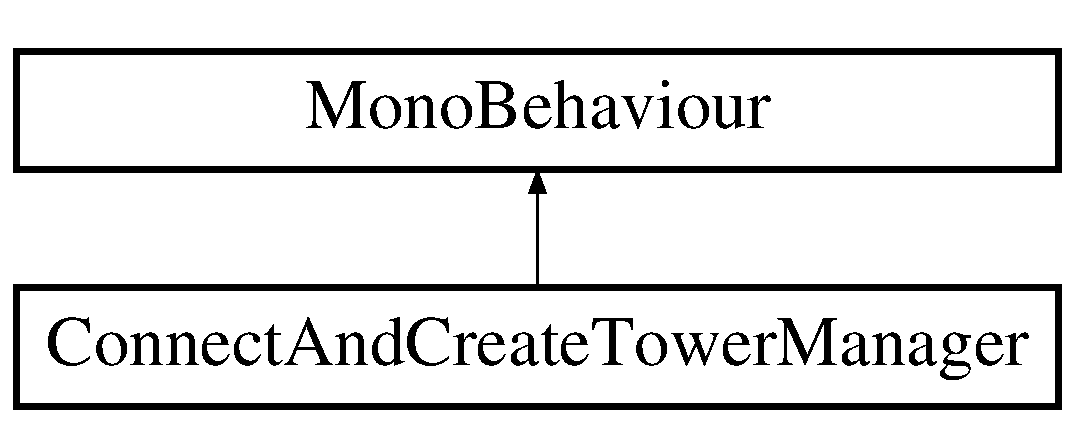
\includegraphics[height=2.000000cm]{class_connect_and_create_tower_manager}
\end{center}
\end{figure}


The documentation for this class was generated from the following file\+:\begin{DoxyCompactItemize}
\item 
/\+Users/benjamin/\+Programmering/\+Android\+H\+M\+D/\+Tower\+V\+R/\+Assets/\+Scripts/\+Custom/\+Game/\+\_\+test/Connect\+And\+Create\+Tower\+Manager.\+cs\end{DoxyCompactItemize}

\hypertarget{class_connect_and_join_test}{}\section{Connect\+And\+Join\+Test Class Reference}
\label{class_connect_and_join_test}\index{Connect\+And\+Join\+Test@{Connect\+And\+Join\+Test}}
Inheritance diagram for Connect\+And\+Join\+Test\+:\begin{figure}[H]
\begin{center}
\leavevmode
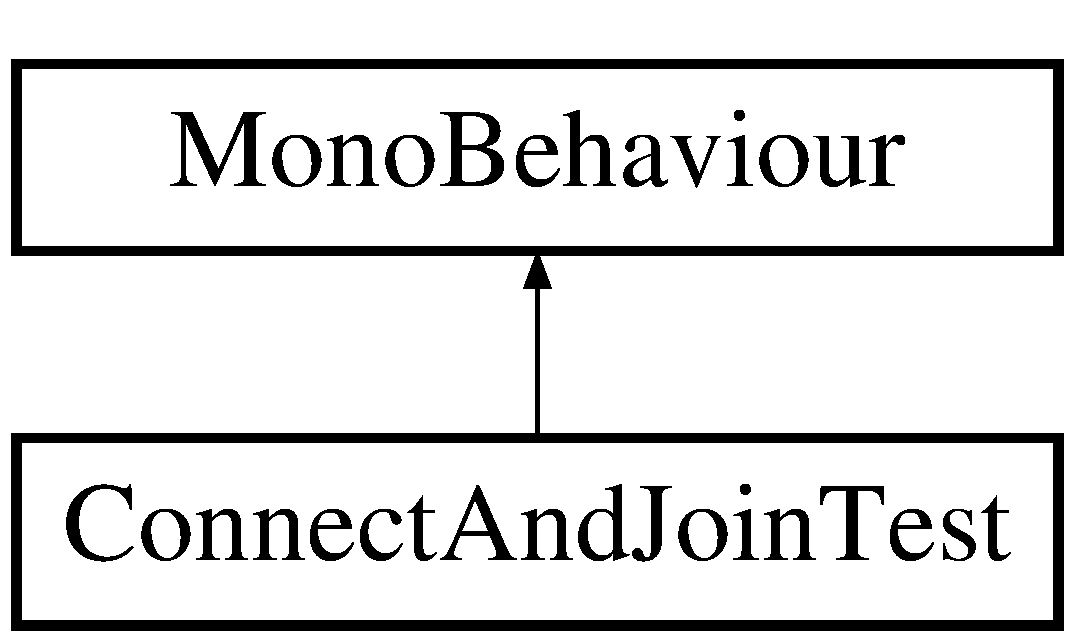
\includegraphics[height=2.000000cm]{class_connect_and_join_test}
\end{center}
\end{figure}
\subsection*{Public Attributes}
\begin{DoxyCompactItemize}
\item 
int {\bfseries scene\+Index}\hypertarget{class_connect_and_join_test_a0861f0b04875328996bddd5b8f7c8ba8}{}\label{class_connect_and_join_test_a0861f0b04875328996bddd5b8f7c8ba8}

\item 
int {\bfseries minimum\+Players} = 1\hypertarget{class_connect_and_join_test_a26634289011e3601ab561cadd1bdd569}{}\label{class_connect_and_join_test_a26634289011e3601ab561cadd1bdd569}

\end{DoxyCompactItemize}


The documentation for this class was generated from the following file\+:\begin{DoxyCompactItemize}
\item 
/\+Users/benjamin/\+Programmering/\+Android\+H\+M\+D/\+Tower\+V\+R/\+Assets/\+Scripts/\+Custom/\+Game/\+\_\+test/Connect\+And\+Join\+Test.\+cs\end{DoxyCompactItemize}

\hypertarget{class_create_new_game}{}\section{Create\+New\+Game Class Reference}
\label{class_create_new_game}\index{Create\+New\+Game@{Create\+New\+Game}}
Inheritance diagram for Create\+New\+Game\+:\begin{figure}[H]
\begin{center}
\leavevmode
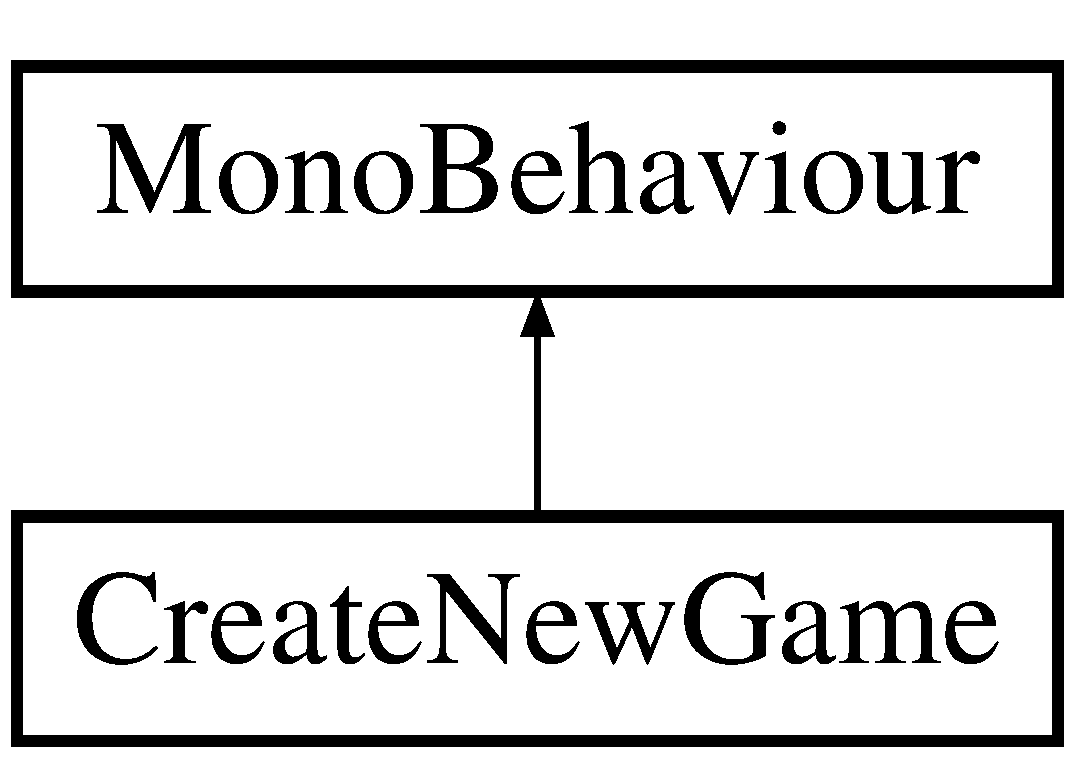
\includegraphics[height=2.000000cm]{class_create_new_game}
\end{center}
\end{figure}
\subsection*{Public Member Functions}
\begin{DoxyCompactItemize}
\item 
void {\bfseries On\+Connected\+To\+Master} ()\hypertarget{class_create_new_game_a0c56a6fe55651aac5376725ffc2f9c0f}{}\label{class_create_new_game_a0c56a6fe55651aac5376725ffc2f9c0f}

\item 
void {\bfseries Start\+New\+Game} ()\hypertarget{class_create_new_game_a2d91e99dfaf2b9e3a91a176314df25f0}{}\label{class_create_new_game_a2d91e99dfaf2b9e3a91a176314df25f0}

\end{DoxyCompactItemize}
\subsection*{Public Attributes}
\begin{DoxyCompactItemize}
\item 
int {\bfseries level\+Index}\hypertarget{class_create_new_game_afa202fe11d0d8a8c6468291951593d38}{}\label{class_create_new_game_afa202fe11d0d8a8c6468291951593d38}

\end{DoxyCompactItemize}


The documentation for this class was generated from the following file\+:\begin{DoxyCompactItemize}
\item 
/\+Users/benjamin/\+Programmering/\+Android\+H\+M\+D/\+Tower\+V\+R/\+Assets/\+Scripts/\+Custom/\+Game/\+Network/Create\+New\+Game.\+cs\end{DoxyCompactItemize}

\hypertarget{class_fading}{}\section{Fading Class Reference}
\label{class_fading}\index{Fading@{Fading}}
Inheritance diagram for Fading\+:\begin{figure}[H]
\begin{center}
\leavevmode
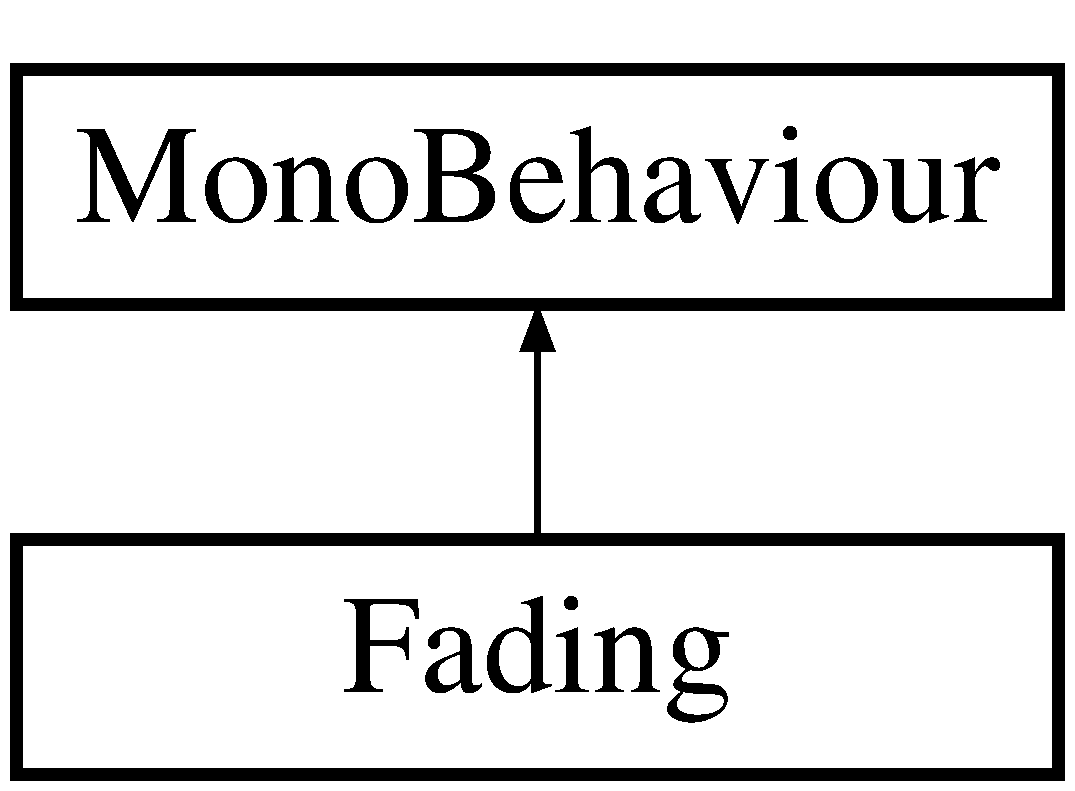
\includegraphics[height=2.000000cm]{class_fading}
\end{center}
\end{figure}
\subsection*{Public Member Functions}
\begin{DoxyCompactItemize}
\item 
float {\bfseries Begin\+Fade} (int direction)\hypertarget{class_fading_aad79c9805adb309dfca9c35956a6539f}{}\label{class_fading_aad79c9805adb309dfca9c35956a6539f}

\end{DoxyCompactItemize}
\subsection*{Public Attributes}
\begin{DoxyCompactItemize}
\item 
Texture2D {\bfseries fade\+Out\+Texture}\hypertarget{class_fading_aaba5de61bbf5cd88b53a8d2b81f074a1}{}\label{class_fading_aaba5de61bbf5cd88b53a8d2b81f074a1}

\item 
float {\bfseries fade\+Speed} = 0.\+0f\hypertarget{class_fading_a4850e50beaca24d0a3266221a36f1e5a}{}\label{class_fading_a4850e50beaca24d0a3266221a36f1e5a}

\end{DoxyCompactItemize}


The documentation for this class was generated from the following file\+:\begin{DoxyCompactItemize}
\item 
/\+Users/benjamin/\+Programmering/\+Android\+H\+M\+D/\+Tower\+V\+R/\+Assets/\+Scripts/\+Custom/Fading.\+cs\end{DoxyCompactItemize}

\hypertarget{class_f_p_s_display}{}\section{F\+P\+S\+Display Class Reference}
\label{class_f_p_s_display}\index{F\+P\+S\+Display@{F\+P\+S\+Display}}
Inheritance diagram for F\+P\+S\+Display\+:\begin{figure}[H]
\begin{center}
\leavevmode
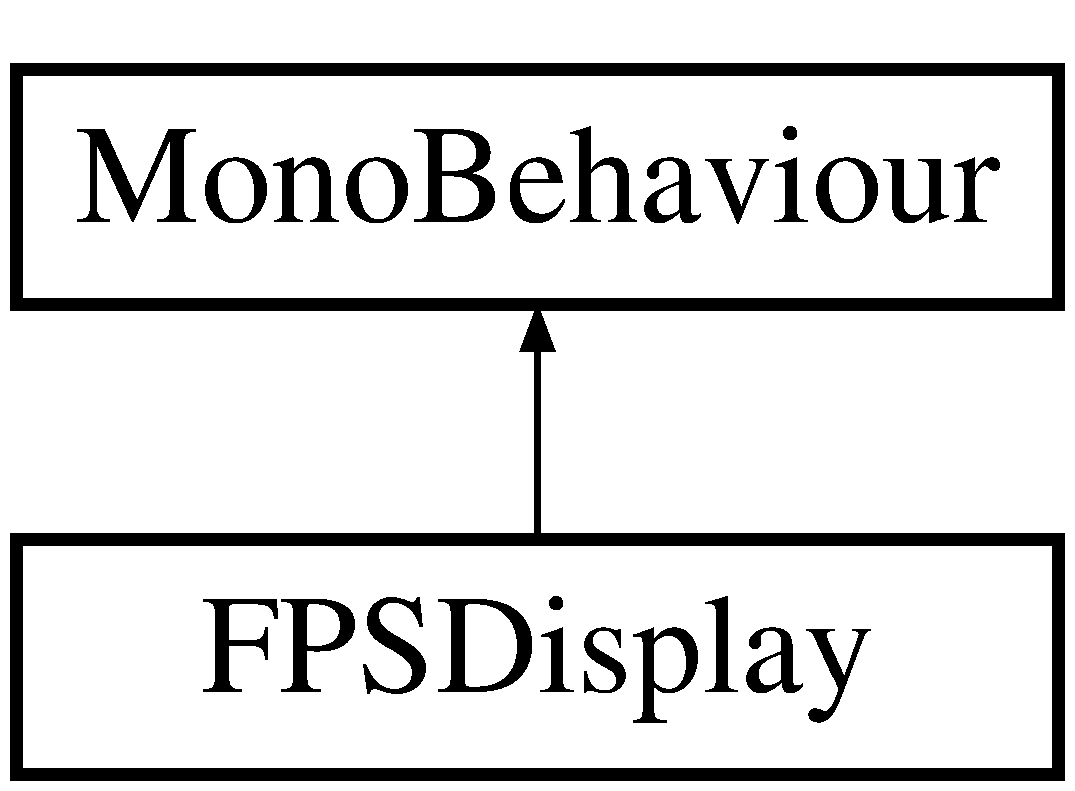
\includegraphics[height=2.000000cm]{class_f_p_s_display}
\end{center}
\end{figure}


The documentation for this class was generated from the following file\+:\begin{DoxyCompactItemize}
\item 
/\+Users/benjamin/\+Programmering/\+Android\+H\+M\+D/\+Tower\+V\+R/\+Assets/\+Scripts/\+Custom/\+Generic/F\+P\+S\+Display.\+cs\end{DoxyCompactItemize}

\hypertarget{class_tower_v_r_1_1_game_state}{}\section{Tower\+V\+R.\+Game\+State Class Reference}
\label{class_tower_v_r_1_1_game_state}\index{Tower\+V\+R.\+Game\+State@{Tower\+V\+R.\+Game\+State}}
\subsection*{Static Public Member Functions}
\begin{DoxyCompactItemize}
\item 
static bool {\bfseries Is\+Valid} (int potential\+Game\+State)\hypertarget{class_tower_v_r_1_1_game_state_a6fc01d6c810e87cbf1c2437555bbf57c}{}\label{class_tower_v_r_1_1_game_state_a6fc01d6c810e87cbf1c2437555bbf57c}

\item 
static string {\bfseries To\+String} (int game\+State)\hypertarget{class_tower_v_r_1_1_game_state_ac8a1ed13699e9c5f45a5817ba67016d3}{}\label{class_tower_v_r_1_1_game_state_ac8a1ed13699e9c5f45a5817ba67016d3}

\end{DoxyCompactItemize}
\subsection*{Public Attributes}
\begin{DoxyCompactItemize}
\item 
const int {\bfseries Awaiting\+Players} = 0\hypertarget{class_tower_v_r_1_1_game_state_ae1c3652510fbccdbd9e27881186d048f}{}\label{class_tower_v_r_1_1_game_state_ae1c3652510fbccdbd9e27881186d048f}

\item 
const int {\bfseries All\+Players\+Ready} = 1\hypertarget{class_tower_v_r_1_1_game_state_a980af313c89a7a078865487cb41cecc1}{}\label{class_tower_v_r_1_1_game_state_a980af313c89a7a078865487cb41cecc1}

\item 
const int {\bfseries Countdown} = 2\hypertarget{class_tower_v_r_1_1_game_state_a04401290d6914dcbccd7fb1084d8c218}{}\label{class_tower_v_r_1_1_game_state_a04401290d6914dcbccd7fb1084d8c218}

\item 
const int {\bfseries Running} = 3\hypertarget{class_tower_v_r_1_1_game_state_afa0cb64d0a46d5a76854e5f14fe13124}{}\label{class_tower_v_r_1_1_game_state_afa0cb64d0a46d5a76854e5f14fe13124}

\item 
const int {\bfseries Ended} = 4\hypertarget{class_tower_v_r_1_1_game_state_a5ebc33265691399fa072175e11b8171d}{}\label{class_tower_v_r_1_1_game_state_a5ebc33265691399fa072175e11b8171d}

\item 
const int {\bfseries Stopped} = 5\hypertarget{class_tower_v_r_1_1_game_state_a61e6560948f61cadb59a8f4069654196}{}\label{class_tower_v_r_1_1_game_state_a61e6560948f61cadb59a8f4069654196}

\end{DoxyCompactItemize}


The documentation for this class was generated from the following file\+:\begin{DoxyCompactItemize}
\item 
/\+Users/benjamin/\+Programmering/\+Android\+H\+M\+D/\+Tower\+V\+R/\+Assets/\+Scripts/\+Custom/\+Game/States.\+cs\end{DoxyCompactItemize}

\hypertarget{class_tower_v_r_1_1_game_state_changed_event}{}\section{Tower\+V\+R.\+Game\+State\+Changed\+Event Class Reference}
\label{class_tower_v_r_1_1_game_state_changed_event}\index{Tower\+V\+R.\+Game\+State\+Changed\+Event@{Tower\+V\+R.\+Game\+State\+Changed\+Event}}
Inheritance diagram for Tower\+V\+R.\+Game\+State\+Changed\+Event\+:\begin{figure}[H]
\begin{center}
\leavevmode
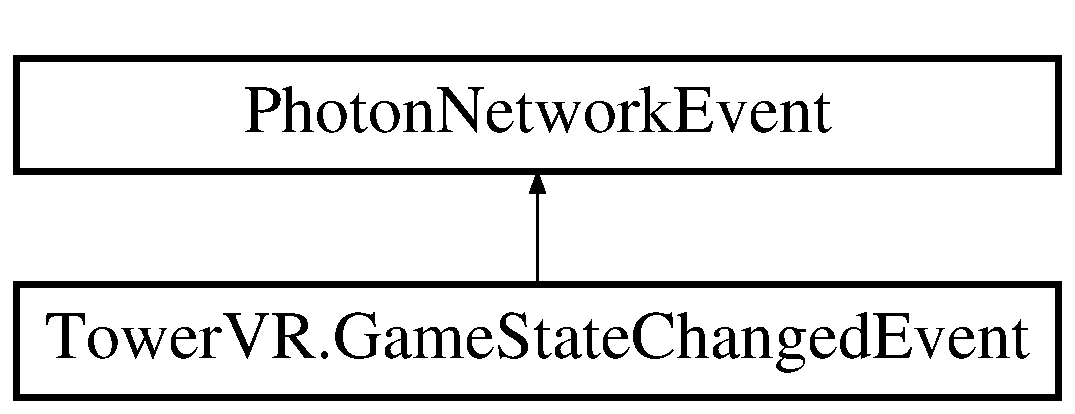
\includegraphics[height=2.000000cm]{class_tower_v_r_1_1_game_state_changed_event}
\end{center}
\end{figure}
\subsection*{Public Member Functions}
\begin{DoxyCompactItemize}
\item 
{\bfseries Game\+State\+Changed\+Event} (int valid\+Game\+State)\hypertarget{class_tower_v_r_1_1_game_state_changed_event_a6f9283ad204a22cb16636b86503ed856}{}\label{class_tower_v_r_1_1_game_state_changed_event_a6f9283ad204a22cb16636b86503ed856}

\end{DoxyCompactItemize}
\subsection*{Static Public Member Functions}
\begin{DoxyCompactItemize}
\item 
static bool \hyperlink{class_tower_v_r_1_1_game_state_changed_event_af0b026428d28bcfe90b00ea8ba4c9c3c}{Try\+Parse} (object obj, out int new\+Game\+State)
\end{DoxyCompactItemize}
\subsection*{Additional Inherited Members}


\subsection{Detailed Description}
An event raised when the master client has changed the game state. 

\subsection{Member Function Documentation}
\index{Tower\+V\+R\+::\+Game\+State\+Changed\+Event@{Tower\+V\+R\+::\+Game\+State\+Changed\+Event}!Try\+Parse@{Try\+Parse}}
\index{Try\+Parse@{Try\+Parse}!Tower\+V\+R\+::\+Game\+State\+Changed\+Event@{Tower\+V\+R\+::\+Game\+State\+Changed\+Event}}
\subsubsection[{\texorpdfstring{Try\+Parse(object obj, out int new\+Game\+State)}{TryParse(object obj, out int newGameState)}}]{\setlength{\rightskip}{0pt plus 5cm}static bool Tower\+V\+R.\+Game\+State\+Changed\+Event.\+Try\+Parse (
\begin{DoxyParamCaption}
\item[{object}]{obj, }
\item[{out int}]{new\+Game\+State}
\end{DoxyParamCaption}
)\hspace{0.3cm}{\ttfamily [static]}}\hypertarget{class_tower_v_r_1_1_game_state_changed_event_af0b026428d28bcfe90b00ea8ba4c9c3c}{}\label{class_tower_v_r_1_1_game_state_changed_event_af0b026428d28bcfe90b00ea8ba4c9c3c}
Tries to parse the contents of the event. 

The documentation for this class was generated from the following file\+:\begin{DoxyCompactItemize}
\item 
/\+Users/benjamin/\+Programmering/\+Android\+H\+M\+D/\+Tower\+V\+R/\+Assets/\+Scripts/\+Custom/\+Game/\+Network/\+Events/Game\+State\+Changed\+Event.\+cs\end{DoxyCompactItemize}

\hypertarget{class_gaze_over}{}\section{Gaze\+Over Class Reference}
\label{class_gaze_over}\index{Gaze\+Over@{Gaze\+Over}}
Inheritance diagram for Gaze\+Over\+:\begin{figure}[H]
\begin{center}
\leavevmode
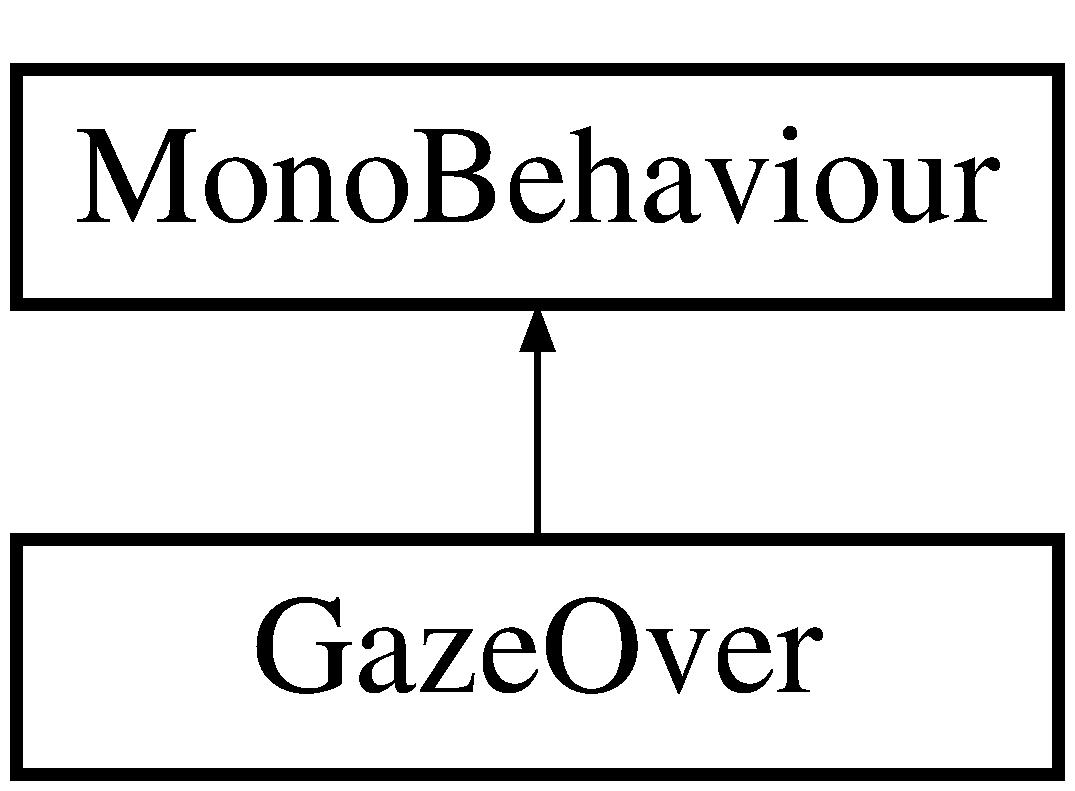
\includegraphics[height=2.000000cm]{class_gaze_over}
\end{center}
\end{figure}
\subsection*{Public Member Functions}
\begin{DoxyCompactItemize}
\item 
void {\bfseries Switch\+Scene} ()\hypertarget{class_gaze_over_a3bb891d7e1c1baf91593d2d975c98ef1}{}\label{class_gaze_over_a3bb891d7e1c1baf91593d2d975c98ef1}

\item 
void {\bfseries Load\+Scene} ()\hypertarget{class_gaze_over_a81b841907b39b75f68a04fef02a5923d}{}\label{class_gaze_over_a81b841907b39b75f68a04fef02a5923d}

\item 
void {\bfseries On\+Pointer\+Enter} ()\hypertarget{class_gaze_over_a8542b157da5e6c98d4500fa96b34e169}{}\label{class_gaze_over_a8542b157da5e6c98d4500fa96b34e169}

\item 
void {\bfseries On\+Pointer\+Exit} ()\hypertarget{class_gaze_over_ac6babe5ebb9a2fe681d559ab64b4f4ad}{}\label{class_gaze_over_ac6babe5ebb9a2fe681d559ab64b4f4ad}

\end{DoxyCompactItemize}
\subsection*{Public Attributes}
\begin{DoxyCompactItemize}
\item 
bool {\bfseries load\+Scene\+For\+All\+Players} = false\hypertarget{class_gaze_over_a1f3d93693093000a182971f54abea678}{}\label{class_gaze_over_a1f3d93693093000a182971f54abea678}

\item 
int {\bfseries level\+Index}\hypertarget{class_gaze_over_a4da14b1f14785e43084c6f5adeb7e641}{}\label{class_gaze_over_a4da14b1f14785e43084c6f5adeb7e641}

\item 
string {\bfseries Level\+Name}\hypertarget{class_gaze_over_a737fc0bbf32691a235d632475daab772}{}\label{class_gaze_over_a737fc0bbf32691a235d632475daab772}

\item 
string {\bfseries Level\+Material1}\hypertarget{class_gaze_over_abaa5c39e1a53eeda5e00a1727da499c6}{}\label{class_gaze_over_abaa5c39e1a53eeda5e00a1727da499c6}

\item 
string {\bfseries Level\+Skybox}\hypertarget{class_gaze_over_ae0fffd931b90309c155a73342ab4c50f}{}\label{class_gaze_over_ae0fffd931b90309c155a73342ab4c50f}

\end{DoxyCompactItemize}


\subsection{Detailed Description}
A class for switching scenes. How to use\+: Make sure your object has a Collider. Add this script and set which scene it should chnage to with index (from build settings). Add Event\+Trigger-\/component and use Pointer Down, Pointer Enter, Pointer Exit for the functions below. Check the box for the load\+Scene\+For\+All\+Players variable to use Photons functionality to sync the loaded scene. 

The documentation for this class was generated from the following file\+:\begin{DoxyCompactItemize}
\item 
/\+Users/benjamin/\+Programmering/\+Android\+H\+M\+D/\+Tower\+V\+R/\+Assets/\+Scripts/\+Custom/Gaze\+Over.\+cs\end{DoxyCompactItemize}

\hypertarget{interface_tower_v_r_1_1_i_tower_game_manager}{}\section{Tower\+V\+R.\+I\+Tower\+Game\+Manager Interface Reference}
\label{interface_tower_v_r_1_1_i_tower_game_manager}\index{Tower\+V\+R.\+I\+Tower\+Game\+Manager@{Tower\+V\+R.\+I\+Tower\+Game\+Manager}}
Inheritance diagram for Tower\+V\+R.\+I\+Tower\+Game\+Manager\+:\begin{figure}[H]
\begin{center}
\leavevmode
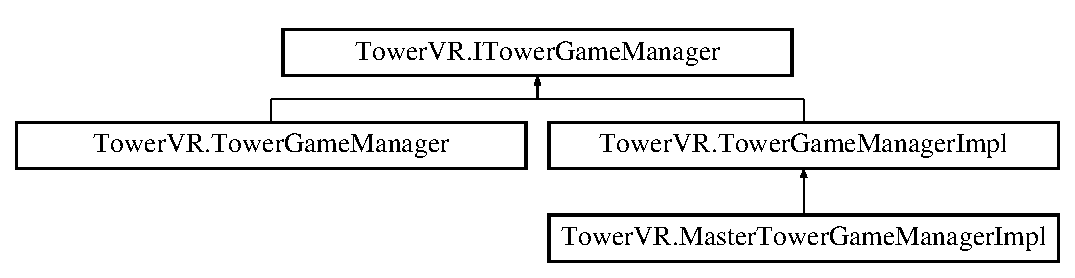
\includegraphics[height=3.000000cm]{interface_tower_v_r_1_1_i_tower_game_manager}
\end{center}
\end{figure}
\subsection*{Public Member Functions}
\begin{DoxyCompactItemize}
\item 
void \hyperlink{interface_tower_v_r_1_1_i_tower_game_manager_a3091c61e8ef71c592a8baf1e611489c0}{notify\+Is\+Ready} ()
\item 
void \hyperlink{interface_tower_v_r_1_1_i_tower_game_manager_a3b5866dd2b9659d65982f4ff651ee2c9}{try\+Start\+Game} ()
\item 
void \hyperlink{interface_tower_v_r_1_1_i_tower_game_manager_aa800aded89d5de4af84321110f6eadd0}{place\+Tower\+Piece} (float positionX, float positionZ, float rotation\+DegreesY)
\end{DoxyCompactItemize}


\subsection{Detailed Description}
Interface to the class that controls the game logic.

The class handles\+:
\begin{DoxyItemize}
\item Game state\+: is the game running? Has it ended?
\item Turn state\+: what action is the current player doing?
\item Turn order\+: In what order does the players play? Has anyone lost yet?
\item Scores
\end{DoxyItemize}

The implementing class is either a local instance (if the current client is the master client), or a remote instance (if the current client is N\+OT the master client). 

\subsection{Member Function Documentation}
\index{Tower\+V\+R\+::\+I\+Tower\+Game\+Manager@{Tower\+V\+R\+::\+I\+Tower\+Game\+Manager}!notify\+Is\+Ready@{notify\+Is\+Ready}}
\index{notify\+Is\+Ready@{notify\+Is\+Ready}!Tower\+V\+R\+::\+I\+Tower\+Game\+Manager@{Tower\+V\+R\+::\+I\+Tower\+Game\+Manager}}
\subsubsection[{\texorpdfstring{notify\+Is\+Ready()}{notifyIsReady()}}]{\setlength{\rightskip}{0pt plus 5cm}void Tower\+V\+R.\+I\+Tower\+Game\+Manager.\+notify\+Is\+Ready (
\begin{DoxyParamCaption}
{}
\end{DoxyParamCaption}
)}\hypertarget{interface_tower_v_r_1_1_i_tower_game_manager_a3091c61e8ef71c592a8baf1e611489c0}{}\label{interface_tower_v_r_1_1_i_tower_game_manager_a3091c61e8ef71c592a8baf1e611489c0}
Call this to notify that this client is ready to start the game. 

Implemented in \hyperlink{class_tower_v_r_1_1_tower_game_manager_impl_ad4a2f3ff8f70fc26602d0c872d5cc36c}{Tower\+V\+R.\+Tower\+Game\+Manager\+Impl}, \hyperlink{class_tower_v_r_1_1_tower_game_manager_a7ea173c143c836423cc25e8f0eed970d}{Tower\+V\+R.\+Tower\+Game\+Manager}, and \hyperlink{class_tower_v_r_1_1_master_tower_game_manager_impl_a318dcef324a58787554cebe80c50ef64}{Tower\+V\+R.\+Master\+Tower\+Game\+Manager\+Impl}.

\index{Tower\+V\+R\+::\+I\+Tower\+Game\+Manager@{Tower\+V\+R\+::\+I\+Tower\+Game\+Manager}!place\+Tower\+Piece@{place\+Tower\+Piece}}
\index{place\+Tower\+Piece@{place\+Tower\+Piece}!Tower\+V\+R\+::\+I\+Tower\+Game\+Manager@{Tower\+V\+R\+::\+I\+Tower\+Game\+Manager}}
\subsubsection[{\texorpdfstring{place\+Tower\+Piece(float position\+X, float position\+Z, float rotation\+Degrees\+Y)}{placeTowerPiece(float positionX, float positionZ, float rotationDegreesY)}}]{\setlength{\rightskip}{0pt plus 5cm}void Tower\+V\+R.\+I\+Tower\+Game\+Manager.\+place\+Tower\+Piece (
\begin{DoxyParamCaption}
\item[{float}]{positionX, }
\item[{float}]{positionZ, }
\item[{float}]{rotation\+DegreesY}
\end{DoxyParamCaption}
)}\hypertarget{interface_tower_v_r_1_1_i_tower_game_manager_aa800aded89d5de4af84321110f6eadd0}{}\label{interface_tower_v_r_1_1_i_tower_game_manager_aa800aded89d5de4af84321110f6eadd0}
Call this to place a tower piece. Will fail silently if it is not the client\textquotesingle{}s turn. 

Implemented in \hyperlink{class_tower_v_r_1_1_tower_game_manager_impl_a47563c59b6d436c05a1f70c16aeb30e9}{Tower\+V\+R.\+Tower\+Game\+Manager\+Impl}, \hyperlink{class_tower_v_r_1_1_master_tower_game_manager_impl_a653a15c9e2af6c11bbd9678cd54a716b}{Tower\+V\+R.\+Master\+Tower\+Game\+Manager\+Impl}, and \hyperlink{class_tower_v_r_1_1_tower_game_manager_aaa476cfb148a19c6579c38823dd37fd3}{Tower\+V\+R.\+Tower\+Game\+Manager}.

\index{Tower\+V\+R\+::\+I\+Tower\+Game\+Manager@{Tower\+V\+R\+::\+I\+Tower\+Game\+Manager}!try\+Start\+Game@{try\+Start\+Game}}
\index{try\+Start\+Game@{try\+Start\+Game}!Tower\+V\+R\+::\+I\+Tower\+Game\+Manager@{Tower\+V\+R\+::\+I\+Tower\+Game\+Manager}}
\subsubsection[{\texorpdfstring{try\+Start\+Game()}{tryStartGame()}}]{\setlength{\rightskip}{0pt plus 5cm}void Tower\+V\+R.\+I\+Tower\+Game\+Manager.\+try\+Start\+Game (
\begin{DoxyParamCaption}
{}
\end{DoxyParamCaption}
)}\hypertarget{interface_tower_v_r_1_1_i_tower_game_manager_a3b5866dd2b9659d65982f4ff651ee2c9}{}\label{interface_tower_v_r_1_1_i_tower_game_manager_a3b5866dd2b9659d65982f4ff651ee2c9}
Tries to start the game. Will fail silently. If it succeeds the client will be alerted through its Game\+State\+Changed\+Handler. 

Implemented in \hyperlink{class_tower_v_r_1_1_tower_game_manager_impl_a04ad123026136abf9c009ff4c03937dc}{Tower\+V\+R.\+Tower\+Game\+Manager\+Impl}, \hyperlink{class_tower_v_r_1_1_master_tower_game_manager_impl_a43cb29dc14b7d9dcd90b5826c49a380d}{Tower\+V\+R.\+Master\+Tower\+Game\+Manager\+Impl}, and \hyperlink{class_tower_v_r_1_1_tower_game_manager_a489f27c61ec3d5c29ac56fea0a024cf6}{Tower\+V\+R.\+Tower\+Game\+Manager}.



The documentation for this interface was generated from the following file\+:\begin{DoxyCompactItemize}
\item 
/\+Users/benjamin/\+Programmering/\+Android\+H\+M\+D/\+Tower\+V\+R/\+Assets/\+Scripts/\+Custom/\+Game/\+Tower/\+Manager/I\+Tower\+Game\+Manager.\+cs\end{DoxyCompactItemize}

\hypertarget{class_join_server}{}\section{Join\+Server Class Reference}
\label{class_join_server}\index{Join\+Server@{Join\+Server}}
Inheritance diagram for Join\+Server\+:\begin{figure}[H]
\begin{center}
\leavevmode
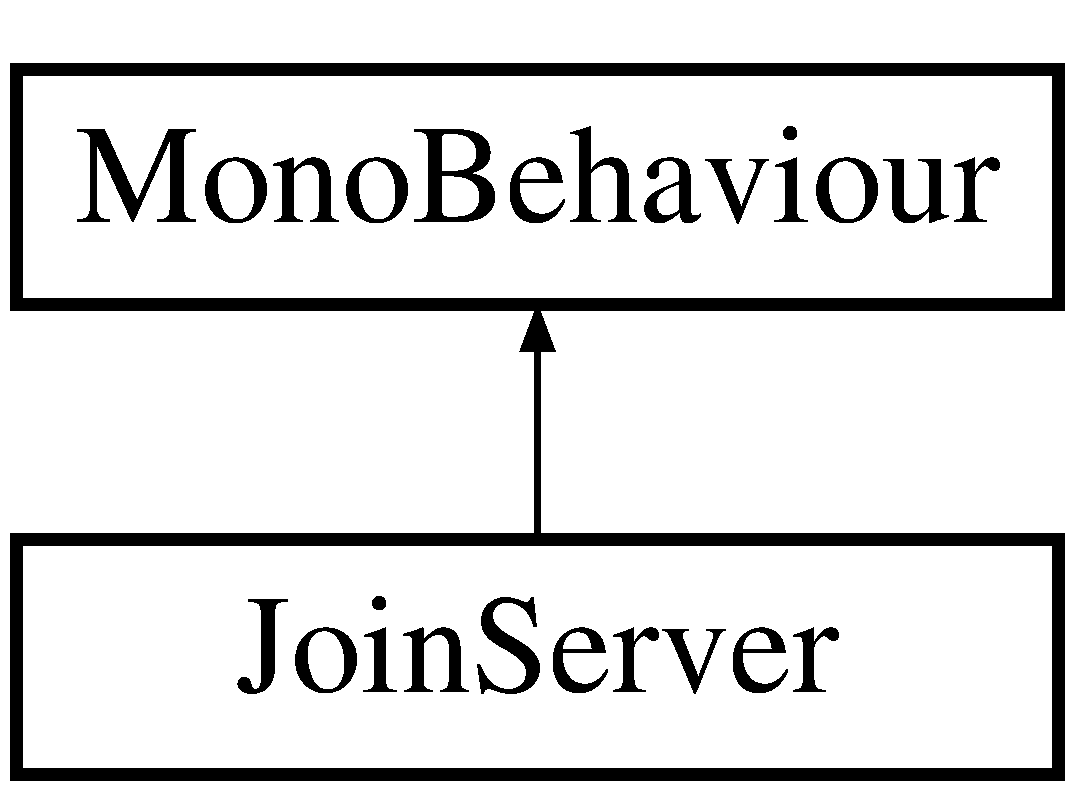
\includegraphics[height=2.000000cm]{class_join_server}
\end{center}
\end{figure}
\subsection*{Public Member Functions}
\begin{DoxyCompactItemize}
\item 
void {\bfseries join\+Server} ()\hypertarget{class_join_server_a20d8990c5457536a20f14a53f327d3c9}{}\label{class_join_server_a20d8990c5457536a20f14a53f327d3c9}

\end{DoxyCompactItemize}
\subsection*{Public Attributes}
\begin{DoxyCompactItemize}
\item 
Text\+Mesh {\bfseries text}\hypertarget{class_join_server_aba960f7e76054c4ebaf1e5c6243a86a9}{}\label{class_join_server_aba960f7e76054c4ebaf1e5c6243a86a9}

\item 
int {\bfseries Level\+Index}\hypertarget{class_join_server_ae9bc9f5b85b97db6f4a061fe47951dac}{}\label{class_join_server_ae9bc9f5b85b97db6f4a061fe47951dac}

\end{DoxyCompactItemize}


The documentation for this class was generated from the following file\+:\begin{DoxyCompactItemize}
\item 
/\+Users/benjamin/\+Programmering/\+Android\+H\+M\+D/\+Tower\+V\+R/\+Assets/\+Scripts/\+Custom/\+Game/\+Network/Join\+Server.\+cs\end{DoxyCompactItemize}

\hypertarget{class_vuforia_1_1_lost_tracking}{}\section{Vuforia.\+Lost\+Tracking Class Reference}
\label{class_vuforia_1_1_lost_tracking}\index{Vuforia.\+Lost\+Tracking@{Vuforia.\+Lost\+Tracking}}
Inheritance diagram for Vuforia.\+Lost\+Tracking\+:\begin{figure}[H]
\begin{center}
\leavevmode
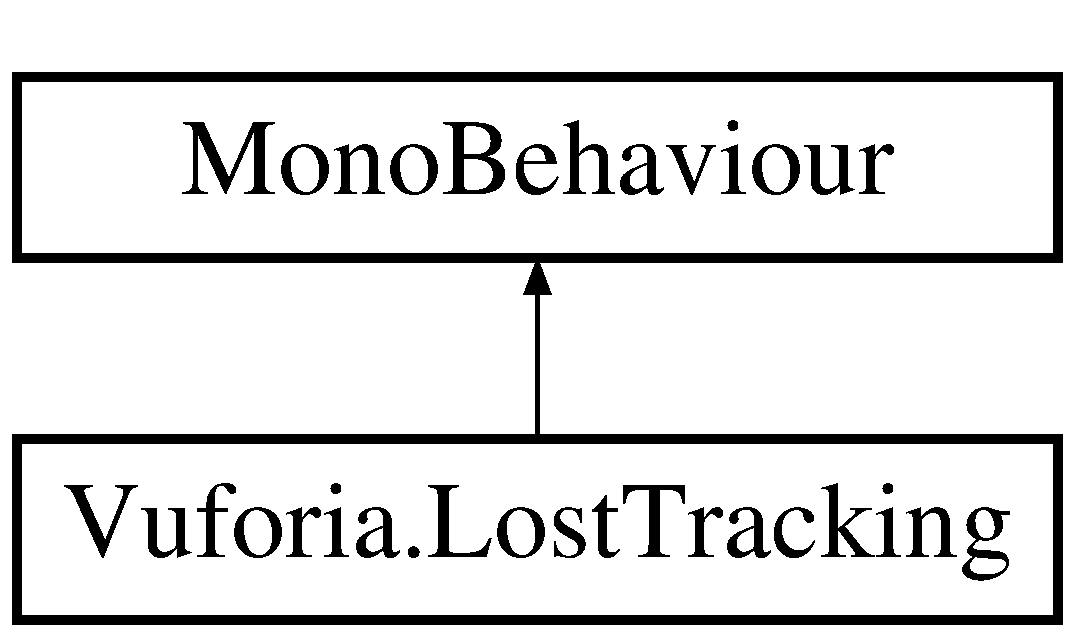
\includegraphics[height=2.000000cm]{class_vuforia_1_1_lost_tracking}
\end{center}
\end{figure}
\subsection*{Public Attributes}
\begin{DoxyCompactItemize}
\item 
Cardboard {\bfseries my\+Cardboard}\hypertarget{class_vuforia_1_1_lost_tracking_a579fe3de0682d2ab61f5cd8ddaaa2d52}{}\label{class_vuforia_1_1_lost_tracking_a579fe3de0682d2ab61f5cd8ddaaa2d52}

\item 
Camera {\bfseries my\+Camera}\hypertarget{class_vuforia_1_1_lost_tracking_a62c8a70332b1f0127cf3bb5f05ae92c1}{}\label{class_vuforia_1_1_lost_tracking_a62c8a70332b1f0127cf3bb5f05ae92c1}

\end{DoxyCompactItemize}


The documentation for this class was generated from the following file\+:\begin{DoxyCompactItemize}
\item 
/\+Users/benjamin/\+Programmering/\+Android\+H\+M\+D/\+Tower\+V\+R/\+Assets/\+Scripts/\+Custom/\+Generic/Lost\+Tracking.\+cs\end{DoxyCompactItemize}

\hypertarget{class_master_client_only_behaviour}{}\section{Master\+Client\+Only\+Behaviour Class Reference}
\label{class_master_client_only_behaviour}\index{Master\+Client\+Only\+Behaviour@{Master\+Client\+Only\+Behaviour}}
Inheritance diagram for Master\+Client\+Only\+Behaviour\+:\begin{figure}[H]
\begin{center}
\leavevmode
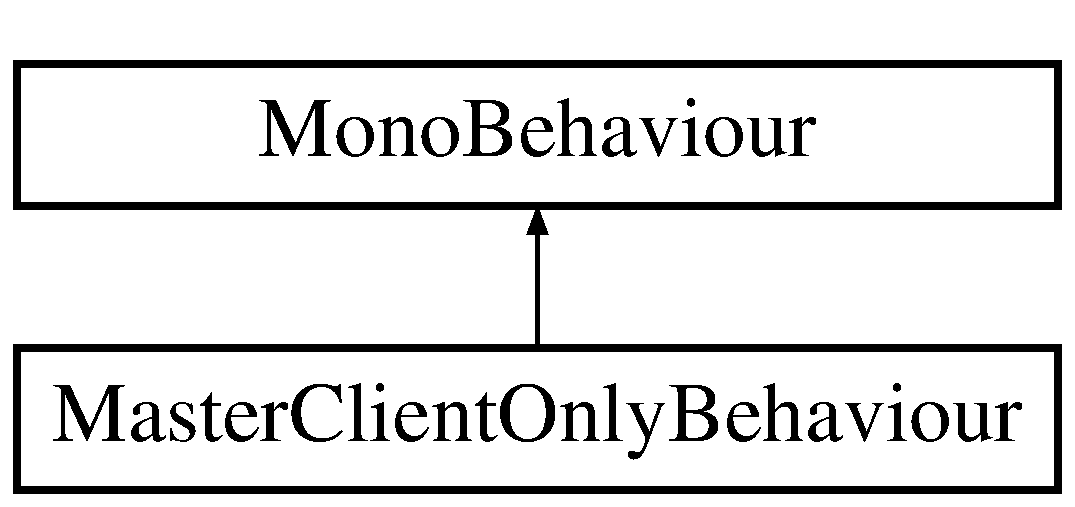
\includegraphics[height=2.000000cm]{class_master_client_only_behaviour}
\end{center}
\end{figure}


\subsection{Detailed Description}
Base Behaviour class that only runs on the Photon\+Network master client. 

The documentation for this class was generated from the following file\+:\begin{DoxyCompactItemize}
\item 
/\+Users/benjamin/\+Programmering/\+Android\+H\+M\+D/\+Tower\+V\+R/\+Assets/\+Scripts/\+Custom/\+Generic/Master\+Client\+Only\+Behaviour.\+cs\end{DoxyCompactItemize}

\hypertarget{class_tower_v_r_1_1_master_client_only_behaviour}{}\section{Tower\+V\+R.\+Master\+Client\+Only\+Behaviour Class Reference}
\label{class_tower_v_r_1_1_master_client_only_behaviour}\index{Tower\+V\+R.\+Master\+Client\+Only\+Behaviour@{Tower\+V\+R.\+Master\+Client\+Only\+Behaviour}}
Inheritance diagram for Tower\+V\+R.\+Master\+Client\+Only\+Behaviour\+:\begin{figure}[H]
\begin{center}
\leavevmode
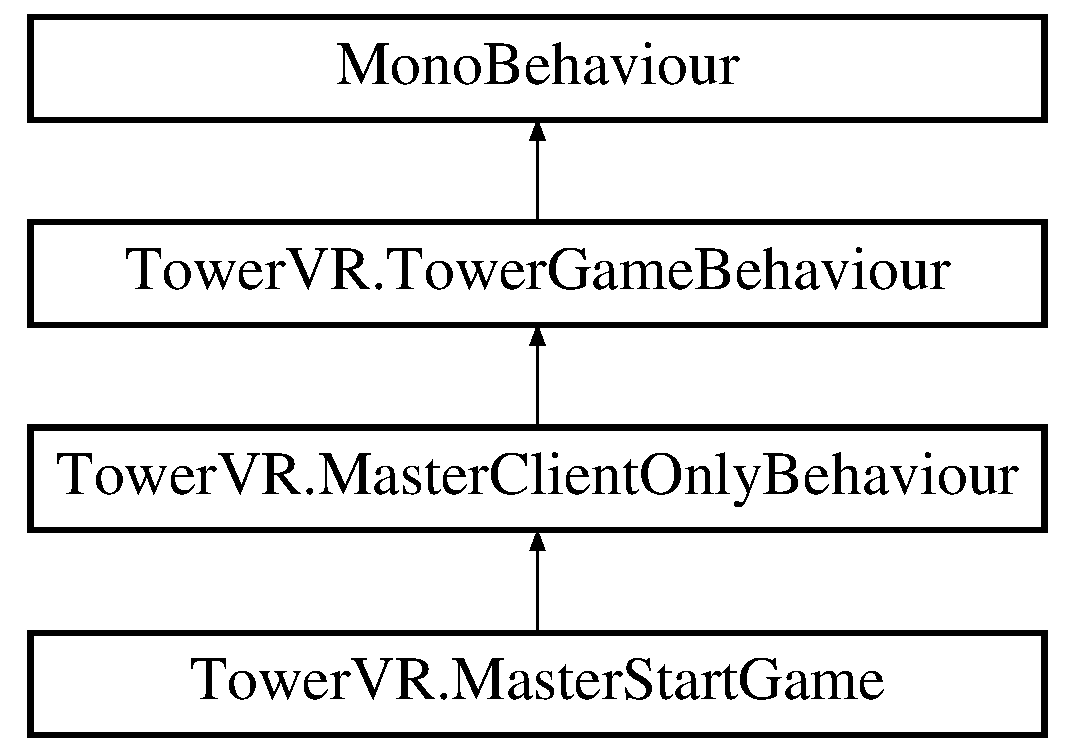
\includegraphics[height=4.000000cm]{class_tower_v_r_1_1_master_client_only_behaviour}
\end{center}
\end{figure}
\subsection*{Additional Inherited Members}


\subsection{Detailed Description}
Base Behaviour class that only runs on the Photon\+Network master client. 

The documentation for this class was generated from the following file\+:\begin{DoxyCompactItemize}
\item 
/\+Users/benjamin/\+Programmering/\+Android\+H\+M\+D/\+Tower\+V\+R/\+Assets/\+Scripts/\+Custom/\+Game/\+Tower/Master\+Client\+Only\+Behaviour.\+cs\end{DoxyCompactItemize}

\hypertarget{class_tower_v_r_1_1_master_start_game}{}\section{Tower\+V\+R.\+Master\+Start\+Game Class Reference}
\label{class_tower_v_r_1_1_master_start_game}\index{Tower\+V\+R.\+Master\+Start\+Game@{Tower\+V\+R.\+Master\+Start\+Game}}
Inheritance diagram for Tower\+V\+R.\+Master\+Start\+Game\+:\begin{figure}[H]
\begin{center}
\leavevmode
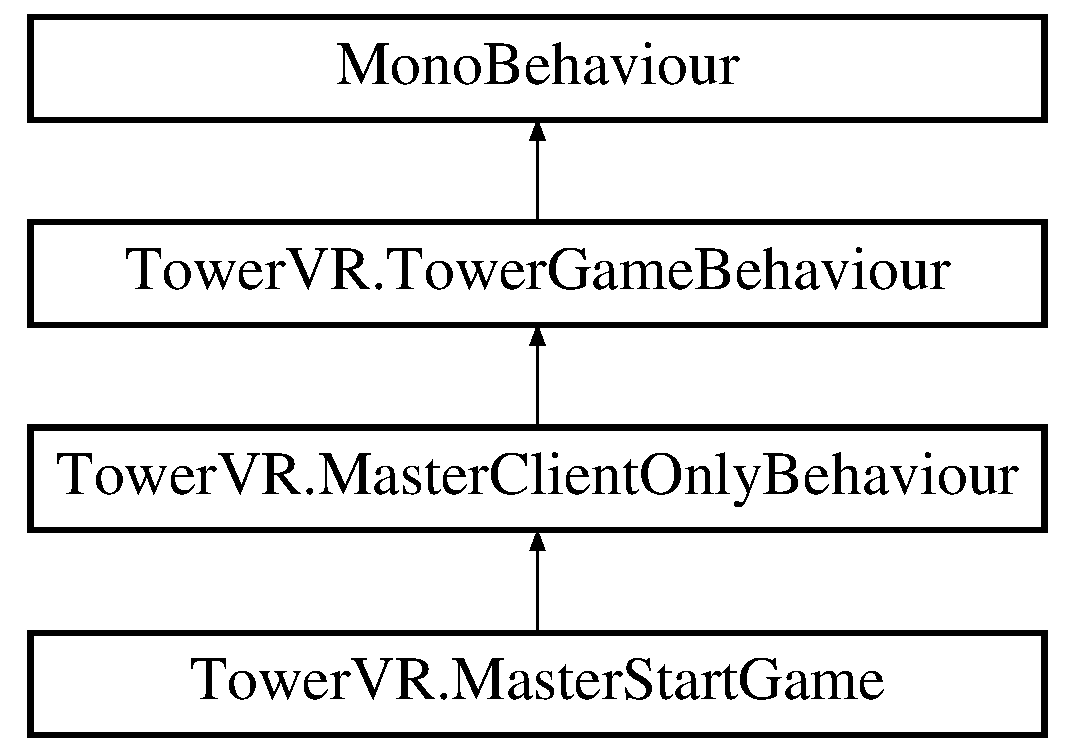
\includegraphics[height=4.000000cm]{class_tower_v_r_1_1_master_start_game}
\end{center}
\end{figure}
\subsection*{Additional Inherited Members}


The documentation for this class was generated from the following file\+:\begin{DoxyCompactItemize}
\item 
/\+Users/benjamin/\+Programmering/\+Android\+H\+M\+D/\+Tower\+V\+R/\+Assets/\+Scripts/\+Custom/\+Game/\+\_\+test/Master\+Start\+Game.\+cs\end{DoxyCompactItemize}

\hypertarget{class_tower_v_r_1_1_master_tower_game_manager_impl}{}\section{Tower\+V\+R.\+Master\+Tower\+Game\+Manager\+Impl Class Reference}
\label{class_tower_v_r_1_1_master_tower_game_manager_impl}\index{Tower\+V\+R.\+Master\+Tower\+Game\+Manager\+Impl@{Tower\+V\+R.\+Master\+Tower\+Game\+Manager\+Impl}}
Inheritance diagram for Tower\+V\+R.\+Master\+Tower\+Game\+Manager\+Impl\+:\begin{figure}[H]
\begin{center}
\leavevmode
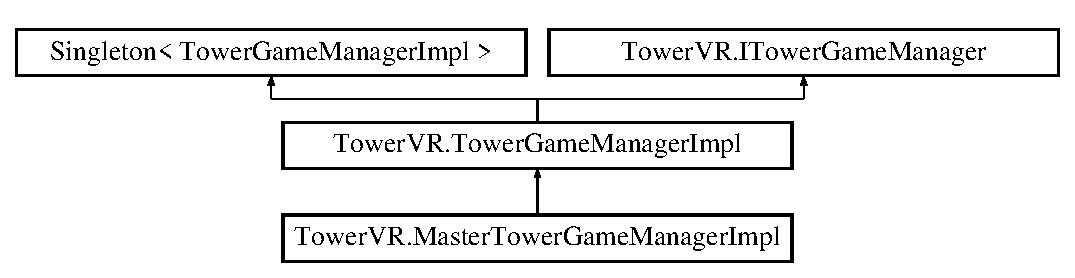
\includegraphics[height=3.000000cm]{class_tower_v_r_1_1_master_tower_game_manager_impl}
\end{center}
\end{figure}
\subsection*{Public Member Functions}
\begin{DoxyCompactItemize}
\item 
sealed override void \hyperlink{class_tower_v_r_1_1_master_tower_game_manager_impl_a318dcef324a58787554cebe80c50ef64}{notify\+Is\+Ready} ()
\item 
sealed override void \hyperlink{class_tower_v_r_1_1_master_tower_game_manager_impl_a43cb29dc14b7d9dcd90b5826c49a380d}{try\+Start\+Game} ()
\item 
sealed override void \hyperlink{class_tower_v_r_1_1_master_tower_game_manager_impl_a653a15c9e2af6c11bbd9678cd54a716b}{place\+Tower\+Piece} (float positionX, float positionZ, float rotation\+DegreesY)
\end{DoxyCompactItemize}
\subsection*{Protected Member Functions}
\begin{DoxyCompactItemize}
\item 
sealed override void {\bfseries Awake} ()\hypertarget{class_tower_v_r_1_1_master_tower_game_manager_impl_a920da97216b0b70d5cc3c9d9a6ef0009}{}\label{class_tower_v_r_1_1_master_tower_game_manager_impl_a920da97216b0b70d5cc3c9d9a6ef0009}

\item 
sealed override void \hyperlink{class_tower_v_r_1_1_master_tower_game_manager_impl_a6b6e868d063e5c3a43908c0f81349cfb}{on\+Event} (byte event\+Code, object content, int sender\+ID)
\item 
void \hyperlink{class_tower_v_r_1_1_master_tower_game_manager_impl_a308a6d258b02fd2c9ee1f9e8d0445dd4}{handle\+Player\+Ready\+Event} (int player\+ID)\hypertarget{class_tower_v_r_1_1_master_tower_game_manager_impl_a308a6d258b02fd2c9ee1f9e8d0445dd4}{}\label{class_tower_v_r_1_1_master_tower_game_manager_impl_a308a6d258b02fd2c9ee1f9e8d0445dd4}

\begin{DoxyCompactList}\small\item\em \hyperlink{class_photon_network_event}{Photon\+Network\+Event} handles ///. \end{DoxyCompactList}\item 
void {\bfseries handle\+Try\+Start\+Game\+Event} (int player\+ID)\hypertarget{class_tower_v_r_1_1_master_tower_game_manager_impl_a8bdba4a2eac7580d0cdc1ee14f9d4623}{}\label{class_tower_v_r_1_1_master_tower_game_manager_impl_a8bdba4a2eac7580d0cdc1ee14f9d4623}

\item 
void {\bfseries handle\+Place\+Tower\+Piece\+Event} (int player\+ID, float posX, float posZ, float rot\+DegreesY)\hypertarget{class_tower_v_r_1_1_master_tower_game_manager_impl_ac6f458a4a2437d060b6940cf01603ebf}{}\label{class_tower_v_r_1_1_master_tower_game_manager_impl_ac6f458a4a2437d060b6940cf01603ebf}

\end{DoxyCompactItemize}
\subsection*{Additional Inherited Members}


\subsection{Detailed Description}
An \hyperlink{interface_tower_v_r_1_1_i_tower_game_manager}{I\+Tower\+Game\+Manager} that represents the master client\textquotesingle{}s instance. This keeps track of the state as well. 

\subsection{Member Function Documentation}
\index{Tower\+V\+R\+::\+Master\+Tower\+Game\+Manager\+Impl@{Tower\+V\+R\+::\+Master\+Tower\+Game\+Manager\+Impl}!notify\+Is\+Ready@{notify\+Is\+Ready}}
\index{notify\+Is\+Ready@{notify\+Is\+Ready}!Tower\+V\+R\+::\+Master\+Tower\+Game\+Manager\+Impl@{Tower\+V\+R\+::\+Master\+Tower\+Game\+Manager\+Impl}}
\subsubsection[{\texorpdfstring{notify\+Is\+Ready()}{notifyIsReady()}}]{\setlength{\rightskip}{0pt plus 5cm}sealed override void Tower\+V\+R.\+Master\+Tower\+Game\+Manager\+Impl.\+notify\+Is\+Ready (
\begin{DoxyParamCaption}
{}
\end{DoxyParamCaption}
)\hspace{0.3cm}{\ttfamily [virtual]}}\hypertarget{class_tower_v_r_1_1_master_tower_game_manager_impl_a318dcef324a58787554cebe80c50ef64}{}\label{class_tower_v_r_1_1_master_tower_game_manager_impl_a318dcef324a58787554cebe80c50ef64}
Overrides the event-\/sending to directly alert this implementation. 

Reimplemented from \hyperlink{class_tower_v_r_1_1_tower_game_manager_impl_ad4a2f3ff8f70fc26602d0c872d5cc36c}{Tower\+V\+R.\+Tower\+Game\+Manager\+Impl}.

\index{Tower\+V\+R\+::\+Master\+Tower\+Game\+Manager\+Impl@{Tower\+V\+R\+::\+Master\+Tower\+Game\+Manager\+Impl}!on\+Event@{on\+Event}}
\index{on\+Event@{on\+Event}!Tower\+V\+R\+::\+Master\+Tower\+Game\+Manager\+Impl@{Tower\+V\+R\+::\+Master\+Tower\+Game\+Manager\+Impl}}
\subsubsection[{\texorpdfstring{on\+Event(byte event\+Code, object content, int sender\+I\+D)}{onEvent(byte eventCode, object content, int senderID)}}]{\setlength{\rightskip}{0pt plus 5cm}sealed override void Tower\+V\+R.\+Master\+Tower\+Game\+Manager\+Impl.\+on\+Event (
\begin{DoxyParamCaption}
\item[{byte}]{event\+Code, }
\item[{object}]{content, }
\item[{int}]{sender\+ID}
\end{DoxyParamCaption}
)\hspace{0.3cm}{\ttfamily [protected]}, {\ttfamily [virtual]}}\hypertarget{class_tower_v_r_1_1_master_tower_game_manager_impl_a6b6e868d063e5c3a43908c0f81349cfb}{}\label{class_tower_v_r_1_1_master_tower_game_manager_impl_a6b6e868d063e5c3a43908c0f81349cfb}
Receives events from the master client and alerts the observer delegates (i.\+e. Tower\+Game\+Behaviours). 

Reimplemented from \hyperlink{class_tower_v_r_1_1_tower_game_manager_impl_a325b500869bda665a71fef31783976be}{Tower\+V\+R.\+Tower\+Game\+Manager\+Impl}.

\index{Tower\+V\+R\+::\+Master\+Tower\+Game\+Manager\+Impl@{Tower\+V\+R\+::\+Master\+Tower\+Game\+Manager\+Impl}!place\+Tower\+Piece@{place\+Tower\+Piece}}
\index{place\+Tower\+Piece@{place\+Tower\+Piece}!Tower\+V\+R\+::\+Master\+Tower\+Game\+Manager\+Impl@{Tower\+V\+R\+::\+Master\+Tower\+Game\+Manager\+Impl}}
\subsubsection[{\texorpdfstring{place\+Tower\+Piece(float position\+X, float position\+Z, float rotation\+Degrees\+Y)}{placeTowerPiece(float positionX, float positionZ, float rotationDegreesY)}}]{\setlength{\rightskip}{0pt plus 5cm}sealed override void Tower\+V\+R.\+Master\+Tower\+Game\+Manager\+Impl.\+place\+Tower\+Piece (
\begin{DoxyParamCaption}
\item[{float}]{positionX, }
\item[{float}]{positionZ, }
\item[{float}]{rotation\+DegreesY}
\end{DoxyParamCaption}
)\hspace{0.3cm}{\ttfamily [virtual]}}\hypertarget{class_tower_v_r_1_1_master_tower_game_manager_impl_a653a15c9e2af6c11bbd9678cd54a716b}{}\label{class_tower_v_r_1_1_master_tower_game_manager_impl_a653a15c9e2af6c11bbd9678cd54a716b}
Overrides the event-\/sending to directly alert this implementation. 

Reimplemented from \hyperlink{class_tower_v_r_1_1_tower_game_manager_impl_a47563c59b6d436c05a1f70c16aeb30e9}{Tower\+V\+R.\+Tower\+Game\+Manager\+Impl}.

\index{Tower\+V\+R\+::\+Master\+Tower\+Game\+Manager\+Impl@{Tower\+V\+R\+::\+Master\+Tower\+Game\+Manager\+Impl}!try\+Start\+Game@{try\+Start\+Game}}
\index{try\+Start\+Game@{try\+Start\+Game}!Tower\+V\+R\+::\+Master\+Tower\+Game\+Manager\+Impl@{Tower\+V\+R\+::\+Master\+Tower\+Game\+Manager\+Impl}}
\subsubsection[{\texorpdfstring{try\+Start\+Game()}{tryStartGame()}}]{\setlength{\rightskip}{0pt plus 5cm}sealed override void Tower\+V\+R.\+Master\+Tower\+Game\+Manager\+Impl.\+try\+Start\+Game (
\begin{DoxyParamCaption}
{}
\end{DoxyParamCaption}
)\hspace{0.3cm}{\ttfamily [virtual]}}\hypertarget{class_tower_v_r_1_1_master_tower_game_manager_impl_a43cb29dc14b7d9dcd90b5826c49a380d}{}\label{class_tower_v_r_1_1_master_tower_game_manager_impl_a43cb29dc14b7d9dcd90b5826c49a380d}
Overrides the event-\/sending to directly alert this implementation. 

Reimplemented from \hyperlink{class_tower_v_r_1_1_tower_game_manager_impl_a04ad123026136abf9c009ff4c03937dc}{Tower\+V\+R.\+Tower\+Game\+Manager\+Impl}.



The documentation for this class was generated from the following file\+:\begin{DoxyCompactItemize}
\item 
/\+Users/benjamin/\+Programmering/\+Android\+H\+M\+D/\+Tower\+V\+R/\+Assets/\+Scripts/\+Custom/\+Game/\+Tower/\+Manager/\+Impl/Master\+Tower\+Game\+Manager\+Impl.\+cs\end{DoxyCompactItemize}

\hypertarget{class_networked_behaviour}{}\section{Networked\+Behaviour Class Reference}
\label{class_networked_behaviour}\index{Networked\+Behaviour@{Networked\+Behaviour}}
Inheritance diagram for Networked\+Behaviour\+:\begin{figure}[H]
\begin{center}
\leavevmode
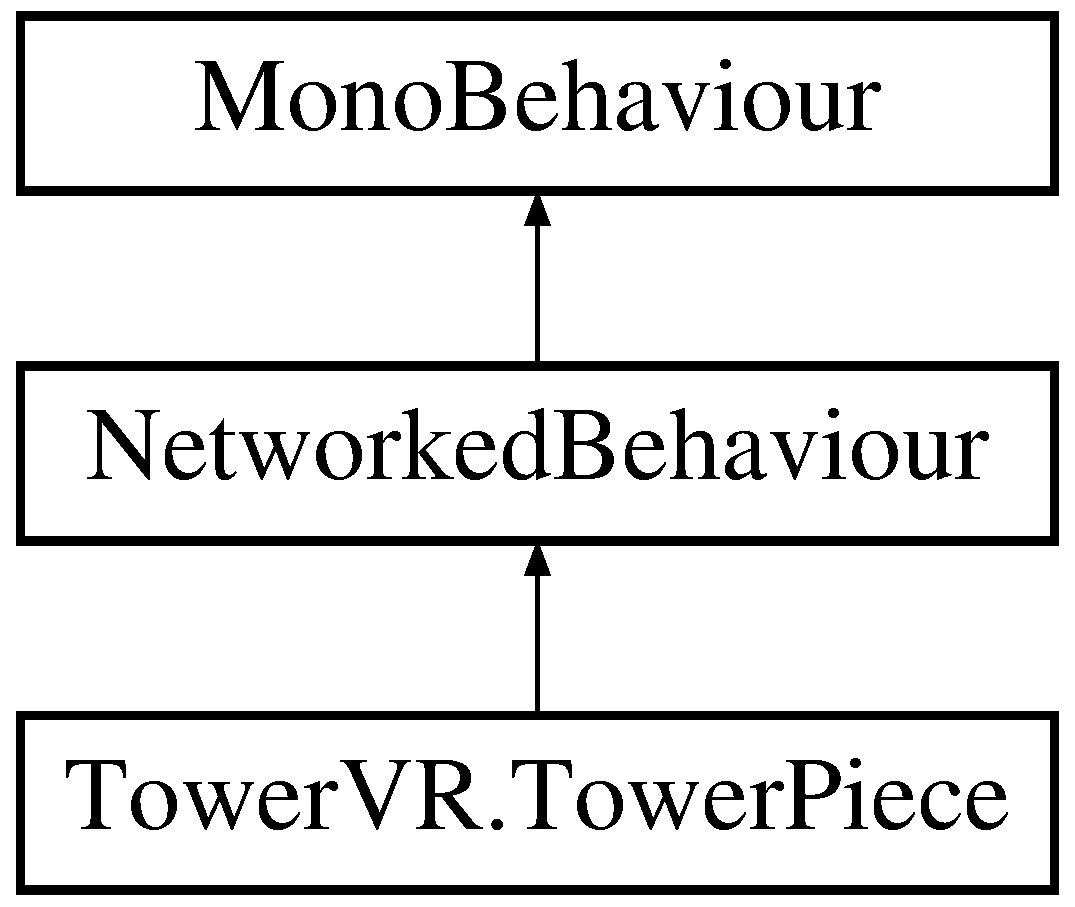
\includegraphics[height=3.000000cm]{class_networked_behaviour}
\end{center}
\end{figure}
\subsection*{Static Public Member Functions}
\begin{DoxyCompactItemize}
\item 
static int {\bfseries Get\+Unique\+Photon\+View\+ID} ()\hypertarget{class_networked_behaviour_a59d7978c054fa5226c43a82566d35877}{}\label{class_networked_behaviour_a59d7978c054fa5226c43a82566d35877}

\end{DoxyCompactItemize}


\subsection{Detailed Description}
Base Behaviour class that ensures the Game\+Object has a Photon\+View and a Photon\+Transform\+View 

The documentation for this class was generated from the following file\+:\begin{DoxyCompactItemize}
\item 
/\+Users/benjamin/\+Programmering/\+Android\+H\+M\+D/\+Tower\+V\+R/\+Assets/\+Scripts/\+Custom/\+Generic/Networked\+Behaviour.\+cs\end{DoxyCompactItemize}

\hypertarget{class_tower_v_r_1_1_network_event_codes}{}\section{Tower\+V\+R.\+Network\+Event\+Codes Class Reference}
\label{class_tower_v_r_1_1_network_event_codes}\index{Tower\+V\+R.\+Network\+Event\+Codes@{Tower\+V\+R.\+Network\+Event\+Codes}}
\subsection*{Static Public Member Functions}
\begin{DoxyCompactItemize}
\item 
static bool {\bfseries Is\+Valid} (byte potential\+Event\+Code)\hypertarget{class_tower_v_r_1_1_network_event_codes_afa0cc00d304b6dfacbb1903d80e0ec52}{}\label{class_tower_v_r_1_1_network_event_codes_afa0cc00d304b6dfacbb1903d80e0ec52}

\end{DoxyCompactItemize}
\subsection*{Public Attributes}
\begin{DoxyCompactItemize}
\item 
const byte {\bfseries Player\+Ready} = 1\hypertarget{class_tower_v_r_1_1_network_event_codes_a6370cf241512b8bd5896b0017c1208f8}{}\label{class_tower_v_r_1_1_network_event_codes_a6370cf241512b8bd5896b0017c1208f8}

\item 
const byte {\bfseries Try\+Start\+Game} = 2\hypertarget{class_tower_v_r_1_1_network_event_codes_aa1759659405e5a0410e84b1ed204b610}{}\label{class_tower_v_r_1_1_network_event_codes_aa1759659405e5a0410e84b1ed204b610}

\item 
const byte {\bfseries Game\+State\+Changed} = 3\hypertarget{class_tower_v_r_1_1_network_event_codes_a9267541fd8c3adc2be663318feee511f}{}\label{class_tower_v_r_1_1_network_event_codes_a9267541fd8c3adc2be663318feee511f}

\item 
const byte {\bfseries Turn\+State\+Changed} = 4\hypertarget{class_tower_v_r_1_1_network_event_codes_a19fa1b33291d600fb7db35704e2d6295}{}\label{class_tower_v_r_1_1_network_event_codes_a19fa1b33291d600fb7db35704e2d6295}

\item 
const byte {\bfseries Next\+Player} = 5\hypertarget{class_tower_v_r_1_1_network_event_codes_a5e272b0571a0a456b50e4b6e193ee7a6}{}\label{class_tower_v_r_1_1_network_event_codes_a5e272b0571a0a456b50e4b6e193ee7a6}

\item 
const byte {\bfseries Score\+Changed} = 6\hypertarget{class_tower_v_r_1_1_network_event_codes_a03ea2ad2c64ba5f91de0de0b02511597}{}\label{class_tower_v_r_1_1_network_event_codes_a03ea2ad2c64ba5f91de0de0b02511597}

\item 
const byte {\bfseries Player\+Lost} = 7\hypertarget{class_tower_v_r_1_1_network_event_codes_afcd1188b4973aae637ba97e42ed8f6f7}{}\label{class_tower_v_r_1_1_network_event_codes_afcd1188b4973aae637ba97e42ed8f6f7}

\item 
const byte {\bfseries Player\+Won} = 8\hypertarget{class_tower_v_r_1_1_network_event_codes_a1a5584045672b73beab84ca8f6f64a95}{}\label{class_tower_v_r_1_1_network_event_codes_a1a5584045672b73beab84ca8f6f64a95}

\item 
const byte {\bfseries Place\+Tower\+Piece} = 0\hypertarget{class_tower_v_r_1_1_network_event_codes_a58643360ed618f18cd05f799674b1b08}{}\label{class_tower_v_r_1_1_network_event_codes_a58643360ed618f18cd05f799674b1b08}

\end{DoxyCompactItemize}


\subsection{Detailed Description}
Constant class containing event codes. The Photon A\+PI specifies the event codes as bytes within the \mbox{[}0, 199\mbox{]} range. 

The documentation for this class was generated from the following file\+:\begin{DoxyCompactItemize}
\item 
/\+Users/benjamin/\+Programmering/\+Android\+H\+M\+D/\+Tower\+V\+R/\+Assets/\+Scripts/\+Custom/\+Game/\+Network/Network\+Event\+Codes.\+cs\end{DoxyCompactItemize}

\hypertarget{class_tower_v_r_1_1_next_player_event}{}\section{Tower\+V\+R.\+Next\+Player\+Event Class Reference}
\label{class_tower_v_r_1_1_next_player_event}\index{Tower\+V\+R.\+Next\+Player\+Event@{Tower\+V\+R.\+Next\+Player\+Event}}
Inheritance diagram for Tower\+V\+R.\+Next\+Player\+Event\+:\begin{figure}[H]
\begin{center}
\leavevmode
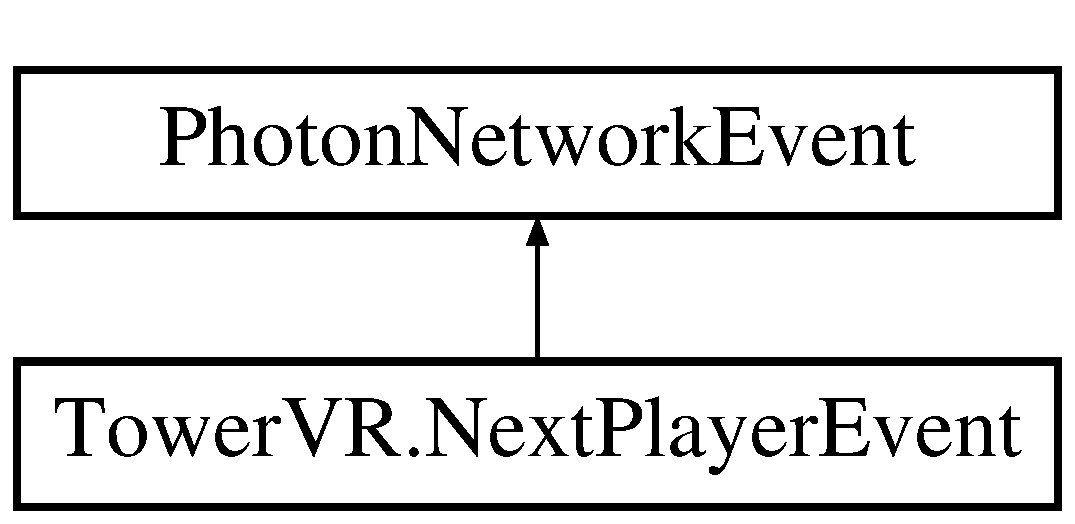
\includegraphics[height=2.000000cm]{class_tower_v_r_1_1_next_player_event}
\end{center}
\end{figure}
\subsection*{Public Member Functions}
\begin{DoxyCompactItemize}
\item 
{\bfseries Next\+Player\+Event} (int next\+Player\+ID)\hypertarget{class_tower_v_r_1_1_next_player_event_a03b2f88c0362a6cbe6a136097ea0709d}{}\label{class_tower_v_r_1_1_next_player_event_a03b2f88c0362a6cbe6a136097ea0709d}

\end{DoxyCompactItemize}
\subsection*{Static Public Member Functions}
\begin{DoxyCompactItemize}
\item 
static bool \hyperlink{class_tower_v_r_1_1_next_player_event_af9e780f7c4231e70f18c90b1911d067d}{Try\+Parse} (object obj, out int next\+Player\+ID)
\end{DoxyCompactItemize}
\subsection*{Additional Inherited Members}


\subsection{Detailed Description}
An event raised when a new player\textquotesingle{}s turn is about to start. 

\subsection{Member Function Documentation}
\index{Tower\+V\+R\+::\+Next\+Player\+Event@{Tower\+V\+R\+::\+Next\+Player\+Event}!Try\+Parse@{Try\+Parse}}
\index{Try\+Parse@{Try\+Parse}!Tower\+V\+R\+::\+Next\+Player\+Event@{Tower\+V\+R\+::\+Next\+Player\+Event}}
\subsubsection[{\texorpdfstring{Try\+Parse(object obj, out int next\+Player\+I\+D)}{TryParse(object obj, out int nextPlayerID)}}]{\setlength{\rightskip}{0pt plus 5cm}static bool Tower\+V\+R.\+Next\+Player\+Event.\+Try\+Parse (
\begin{DoxyParamCaption}
\item[{object}]{obj, }
\item[{out int}]{next\+Player\+ID}
\end{DoxyParamCaption}
)\hspace{0.3cm}{\ttfamily [static]}}\hypertarget{class_tower_v_r_1_1_next_player_event_af9e780f7c4231e70f18c90b1911d067d}{}\label{class_tower_v_r_1_1_next_player_event_af9e780f7c4231e70f18c90b1911d067d}
Tries to parse the contents of the event. 

The documentation for this class was generated from the following file\+:\begin{DoxyCompactItemize}
\item 
/\+Users/benjamin/\+Programmering/\+Android\+H\+M\+D/\+Tower\+V\+R/\+Assets/\+Scripts/\+Custom/\+Game/\+Network/\+Events/Next\+Player\+Event.\+cs\end{DoxyCompactItemize}

\hypertarget{class_photon_network_event}{}\section{Photon\+Network\+Event Class Reference}
\label{class_photon_network_event}\index{Photon\+Network\+Event@{Photon\+Network\+Event}}
Inheritance diagram for Photon\+Network\+Event\+:\begin{figure}[H]
\begin{center}
\leavevmode
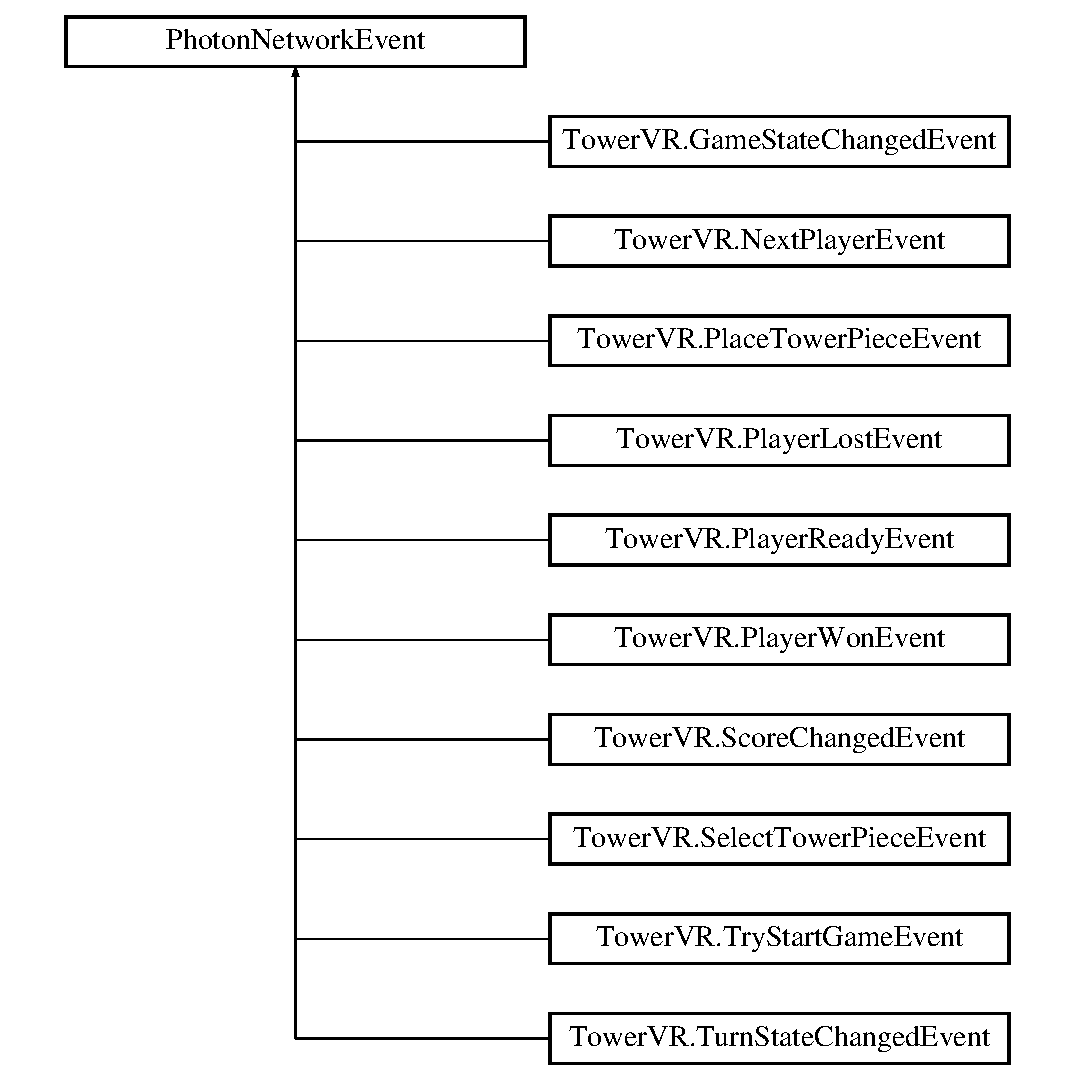
\includegraphics[height=11.000000cm]{class_photon_network_event}
\end{center}
\end{figure}
\subsection*{Public Member Functions}
\begin{DoxyCompactItemize}
\item 
bool {\bfseries try\+Send} ()\hypertarget{class_photon_network_event_acbfe71760048a6edf950f710167b56ca}{}\label{class_photon_network_event_acbfe71760048a6edf950f710167b56ca}

\end{DoxyCompactItemize}
\subsection*{Protected Member Functions}
\begin{DoxyCompactItemize}
\item 
void {\bfseries set\+Receivers} (Receiver\+Group receiver\+Group)\hypertarget{class_photon_network_event_a7344442ecce18c3a78594f9a298a2572}{}\label{class_photon_network_event_a7344442ecce18c3a78594f9a298a2572}

\item 
void {\bfseries set\+Receivers} (params int\mbox{[}$\,$\mbox{]} player\+I\+Ds)\hypertarget{class_photon_network_event_a070870e1683624c335c5a9ecb9cb2b29}{}\label{class_photon_network_event_a070870e1683624c335c5a9ecb9cb2b29}

\item 
virtual bool \hyperlink{class_photon_network_event_a82a5487738983085c9e8ac4116474b43}{content\+Is\+Valid} ()
\end{DoxyCompactItemize}
\subsection*{Properties}
\begin{DoxyCompactItemize}
\item 
byte {\bfseries event\+Code}\hspace{0.3cm}{\ttfamily  \mbox{[}get, set\mbox{]}}\hypertarget{class_photon_network_event_a93db8417c2b97d96ac6541ad2eda3743}{}\label{class_photon_network_event_a93db8417c2b97d96ac6541ad2eda3743}

\item 
object {\bfseries content}\hspace{0.3cm}{\ttfamily  \mbox{[}get, set\mbox{]}}\hypertarget{class_photon_network_event_af40128239b2f9a8fb905f125ddbf5e96}{}\label{class_photon_network_event_af40128239b2f9a8fb905f125ddbf5e96}

\item 
Raise\+Event\+Options {\bfseries event\+Options}\hspace{0.3cm}{\ttfamily  \mbox{[}get, set\mbox{]}}\hypertarget{class_photon_network_event_a03103d069e24a349bf4fc74a493bbeda}{}\label{class_photon_network_event_a03103d069e24a349bf4fc74a493bbeda}

\item 
string {\bfseries try\+Send\+Error}\hspace{0.3cm}{\ttfamily  \mbox{[}get, protected set\mbox{]}}\hypertarget{class_photon_network_event_a26b1e1ac39a121ed6e202eeaaa5e7df1}{}\label{class_photon_network_event_a26b1e1ac39a121ed6e202eeaaa5e7df1}

\end{DoxyCompactItemize}


\subsection{Detailed Description}
Abstract base class for events sent using the Photon A\+PI. 

\subsection{Member Function Documentation}
\index{Photon\+Network\+Event@{Photon\+Network\+Event}!content\+Is\+Valid@{content\+Is\+Valid}}
\index{content\+Is\+Valid@{content\+Is\+Valid}!Photon\+Network\+Event@{Photon\+Network\+Event}}
\subsubsection[{\texorpdfstring{content\+Is\+Valid()}{contentIsValid()}}]{\setlength{\rightskip}{0pt plus 5cm}virtual bool Photon\+Network\+Event.\+content\+Is\+Valid (
\begin{DoxyParamCaption}
{}
\end{DoxyParamCaption}
)\hspace{0.3cm}{\ttfamily [protected]}, {\ttfamily [virtual]}}\hypertarget{class_photon_network_event_a82a5487738983085c9e8ac4116474b43}{}\label{class_photon_network_event_a82a5487738983085c9e8ac4116474b43}
Override this to provide extra content validation. 

Reimplemented in \hyperlink{class_tower_v_r_1_1_select_tower_piece_event_addf1cb68acf541e199df157a32ab25ca}{Tower\+V\+R.\+Select\+Tower\+Piece\+Event}.



The documentation for this class was generated from the following file\+:\begin{DoxyCompactItemize}
\item 
/\+Users/benjamin/\+Programmering/\+Android\+H\+M\+D/\+Tower\+V\+R/\+Assets/\+Scripts/\+Custom/\+Generic/Photon\+Network\+Event.\+cs\end{DoxyCompactItemize}

\hypertarget{class_tower_v_r_1_1_place_tower_piece_event}{}\section{Tower\+V\+R.\+Place\+Tower\+Piece\+Event Class Reference}
\label{class_tower_v_r_1_1_place_tower_piece_event}\index{Tower\+V\+R.\+Place\+Tower\+Piece\+Event@{Tower\+V\+R.\+Place\+Tower\+Piece\+Event}}
Inheritance diagram for Tower\+V\+R.\+Place\+Tower\+Piece\+Event\+:\begin{figure}[H]
\begin{center}
\leavevmode
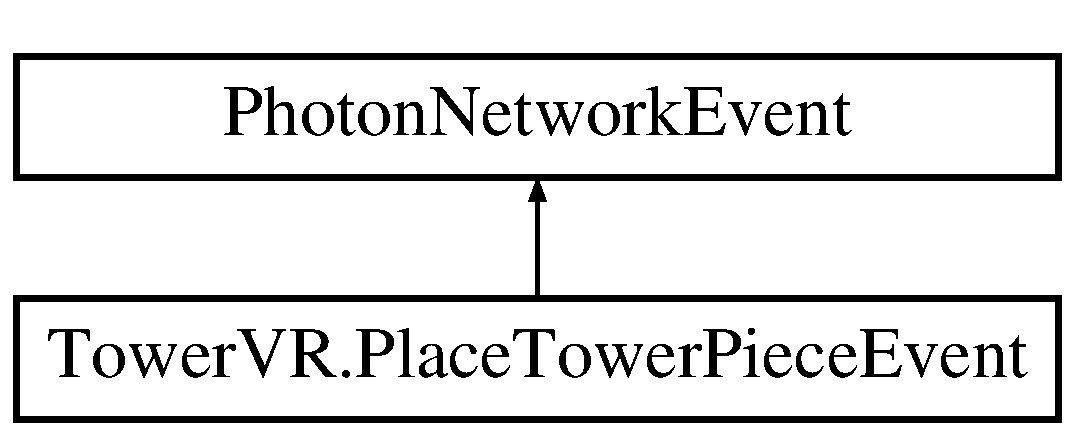
\includegraphics[height=2.000000cm]{class_tower_v_r_1_1_place_tower_piece_event}
\end{center}
\end{figure}
\subsection*{Public Member Functions}
\begin{DoxyCompactItemize}
\item 
{\bfseries Place\+Tower\+Piece\+Event} (float positionX, float positionZ, float rotation\+DegreesY)\hypertarget{class_tower_v_r_1_1_place_tower_piece_event_a3d2c63251ae5eaba62b4ba45ba33aee3}{}\label{class_tower_v_r_1_1_place_tower_piece_event_a3d2c63251ae5eaba62b4ba45ba33aee3}

\end{DoxyCompactItemize}
\subsection*{Static Public Member Functions}
\begin{DoxyCompactItemize}
\item 
static bool \hyperlink{class_tower_v_r_1_1_place_tower_piece_event_a8a17a8e6f863a9d0b0405279d0bb6ed4}{Try\+Parse} (object obj, out float posX, out float posZ, out float rot\+DegreesY)
\end{DoxyCompactItemize}
\subsection*{Additional Inherited Members}


\subsection{Detailed Description}
An event sent to the master client when the current player places his/her current tower piece. 

\subsection{Member Function Documentation}
\index{Tower\+V\+R\+::\+Place\+Tower\+Piece\+Event@{Tower\+V\+R\+::\+Place\+Tower\+Piece\+Event}!Try\+Parse@{Try\+Parse}}
\index{Try\+Parse@{Try\+Parse}!Tower\+V\+R\+::\+Place\+Tower\+Piece\+Event@{Tower\+V\+R\+::\+Place\+Tower\+Piece\+Event}}
\subsubsection[{\texorpdfstring{Try\+Parse(object obj, out float pos\+X, out float pos\+Z, out float rot\+Degrees\+Y)}{TryParse(object obj, out float posX, out float posZ, out float rotDegreesY)}}]{\setlength{\rightskip}{0pt plus 5cm}static bool Tower\+V\+R.\+Place\+Tower\+Piece\+Event.\+Try\+Parse (
\begin{DoxyParamCaption}
\item[{object}]{obj, }
\item[{out float}]{posX, }
\item[{out float}]{posZ, }
\item[{out float}]{rot\+DegreesY}
\end{DoxyParamCaption}
)\hspace{0.3cm}{\ttfamily [static]}}\hypertarget{class_tower_v_r_1_1_place_tower_piece_event_a8a17a8e6f863a9d0b0405279d0bb6ed4}{}\label{class_tower_v_r_1_1_place_tower_piece_event_a8a17a8e6f863a9d0b0405279d0bb6ed4}
Tries to parse the contents of the event. 

The documentation for this class was generated from the following file\+:\begin{DoxyCompactItemize}
\item 
/\+Users/benjamin/\+Programmering/\+Android\+H\+M\+D/\+Tower\+V\+R/\+Assets/\+Scripts/\+Custom/\+Game/\+Network/\+Events/Place\+Tower\+Piece\+Event.\+cs\end{DoxyCompactItemize}

\hypertarget{class_player_camera_movement}{}\section{Player\+Camera\+Movement Class Reference}
\label{class_player_camera_movement}\index{Player\+Camera\+Movement@{Player\+Camera\+Movement}}
Inheritance diagram for Player\+Camera\+Movement\+:\begin{figure}[H]
\begin{center}
\leavevmode
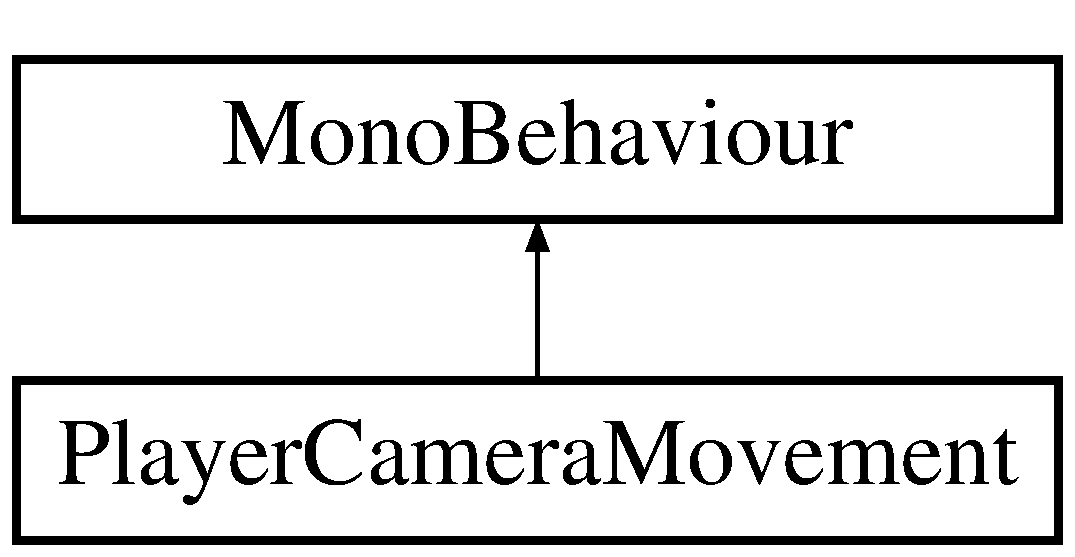
\includegraphics[height=2.000000cm]{class_player_camera_movement}
\end{center}
\end{figure}
\subsection*{Public Attributes}
\begin{DoxyCompactItemize}
\item 
bool {\bfseries debug\+Position} = false\hypertarget{class_player_camera_movement_a617542dd9ab3ec53e2ea169e237e56e3}{}\label{class_player_camera_movement_a617542dd9ab3ec53e2ea169e237e56e3}

\end{DoxyCompactItemize}


\subsection{Detailed Description}
Updates position for a player object by setting its position to each player\textquotesingle{}s client camera position 

The documentation for this class was generated from the following file\+:\begin{DoxyCompactItemize}
\item 
/\+Users/benjamin/\+Programmering/\+Android\+H\+M\+D/\+Tower\+V\+R/\+Assets/\+Scripts/\+Custom/\+Game/\+Network/Player\+Camera\+Movement.\+cs\end{DoxyCompactItemize}

\hypertarget{class_tower_v_r_1_1_player_lost_event}{}\section{Tower\+V\+R.\+Player\+Lost\+Event Class Reference}
\label{class_tower_v_r_1_1_player_lost_event}\index{Tower\+V\+R.\+Player\+Lost\+Event@{Tower\+V\+R.\+Player\+Lost\+Event}}
Inheritance diagram for Tower\+V\+R.\+Player\+Lost\+Event\+:\begin{figure}[H]
\begin{center}
\leavevmode
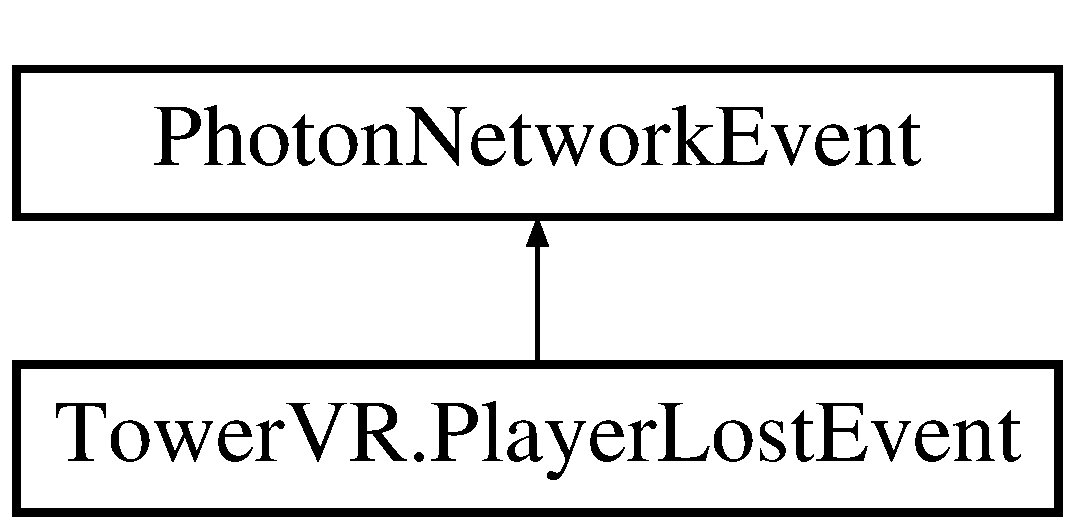
\includegraphics[height=2.000000cm]{class_tower_v_r_1_1_player_lost_event}
\end{center}
\end{figure}
\subsection*{Public Member Functions}
\begin{DoxyCompactItemize}
\item 
{\bfseries Player\+Lost\+Event} (int player\+ID)\hypertarget{class_tower_v_r_1_1_player_lost_event_a4ecf91efaab9b6d6c50dd8946bd3b4c8}{}\label{class_tower_v_r_1_1_player_lost_event_a4ecf91efaab9b6d6c50dd8946bd3b4c8}

\end{DoxyCompactItemize}
\subsection*{Static Public Member Functions}
\begin{DoxyCompactItemize}
\item 
static bool \hyperlink{class_tower_v_r_1_1_player_lost_event_a1a5a7b6b2e4b15c97ae2b0da6be59afd}{Try\+Parse} (object obj, out int player\+ID)
\end{DoxyCompactItemize}
\subsection*{Additional Inherited Members}


\subsection{Detailed Description}
An event raised when a player lost the game. 

\subsection{Member Function Documentation}
\index{Tower\+V\+R\+::\+Player\+Lost\+Event@{Tower\+V\+R\+::\+Player\+Lost\+Event}!Try\+Parse@{Try\+Parse}}
\index{Try\+Parse@{Try\+Parse}!Tower\+V\+R\+::\+Player\+Lost\+Event@{Tower\+V\+R\+::\+Player\+Lost\+Event}}
\subsubsection[{\texorpdfstring{Try\+Parse(object obj, out int player\+I\+D)}{TryParse(object obj, out int playerID)}}]{\setlength{\rightskip}{0pt plus 5cm}static bool Tower\+V\+R.\+Player\+Lost\+Event.\+Try\+Parse (
\begin{DoxyParamCaption}
\item[{object}]{obj, }
\item[{out int}]{player\+ID}
\end{DoxyParamCaption}
)\hspace{0.3cm}{\ttfamily [static]}}\hypertarget{class_tower_v_r_1_1_player_lost_event_a1a5a7b6b2e4b15c97ae2b0da6be59afd}{}\label{class_tower_v_r_1_1_player_lost_event_a1a5a7b6b2e4b15c97ae2b0da6be59afd}
Tries to parse the contents of the event. 

The documentation for this class was generated from the following file\+:\begin{DoxyCompactItemize}
\item 
/\+Users/benjamin/\+Programmering/\+Android\+H\+M\+D/\+Tower\+V\+R/\+Assets/\+Scripts/\+Custom/\+Game/\+Network/\+Events/Player\+Lost\+Event.\+cs\end{DoxyCompactItemize}

\hypertarget{class_tower_v_r_1_1_player_ready_event}{}\section{Tower\+V\+R.\+Player\+Ready\+Event Class Reference}
\label{class_tower_v_r_1_1_player_ready_event}\index{Tower\+V\+R.\+Player\+Ready\+Event@{Tower\+V\+R.\+Player\+Ready\+Event}}
Inheritance diagram for Tower\+V\+R.\+Player\+Ready\+Event\+:\begin{figure}[H]
\begin{center}
\leavevmode
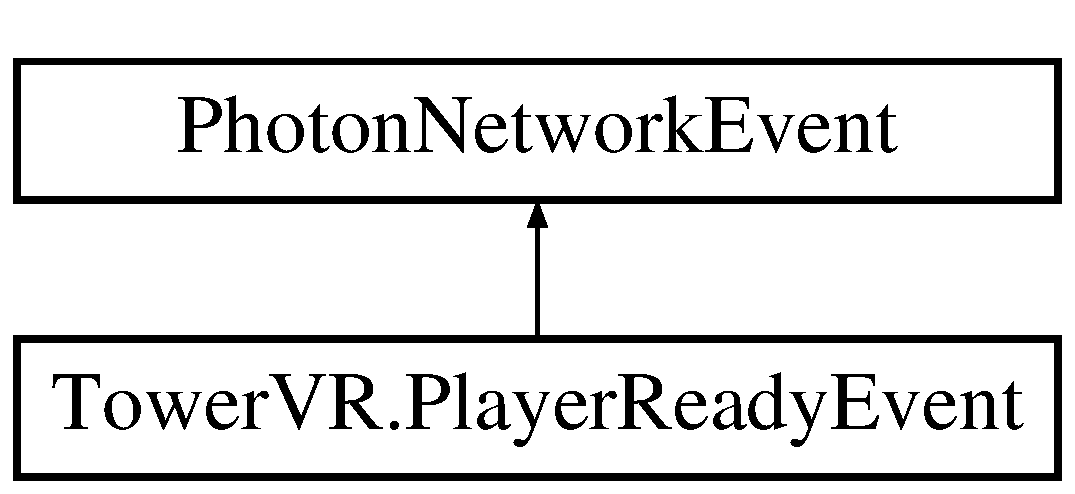
\includegraphics[height=2.000000cm]{class_tower_v_r_1_1_player_ready_event}
\end{center}
\end{figure}
\subsection*{Additional Inherited Members}


\subsection{Detailed Description}
An event raised when the sending player is ready to start the game. 

The documentation for this class was generated from the following file\+:\begin{DoxyCompactItemize}
\item 
/\+Users/benjamin/\+Programmering/\+Android\+H\+M\+D/\+Tower\+V\+R/\+Assets/\+Scripts/\+Custom/\+Game/\+Network/\+Events/Player\+Ready\+Event.\+cs\end{DoxyCompactItemize}

\hypertarget{class_tower_v_r_1_1_player_turn_observer}{}\section{Tower\+V\+R.\+Player\+Turn\+Observer Class Reference}
\label{class_tower_v_r_1_1_player_turn_observer}\index{Tower\+V\+R.\+Player\+Turn\+Observer@{Tower\+V\+R.\+Player\+Turn\+Observer}}
Inheritance diagram for Tower\+V\+R.\+Player\+Turn\+Observer\+:\begin{figure}[H]
\begin{center}
\leavevmode
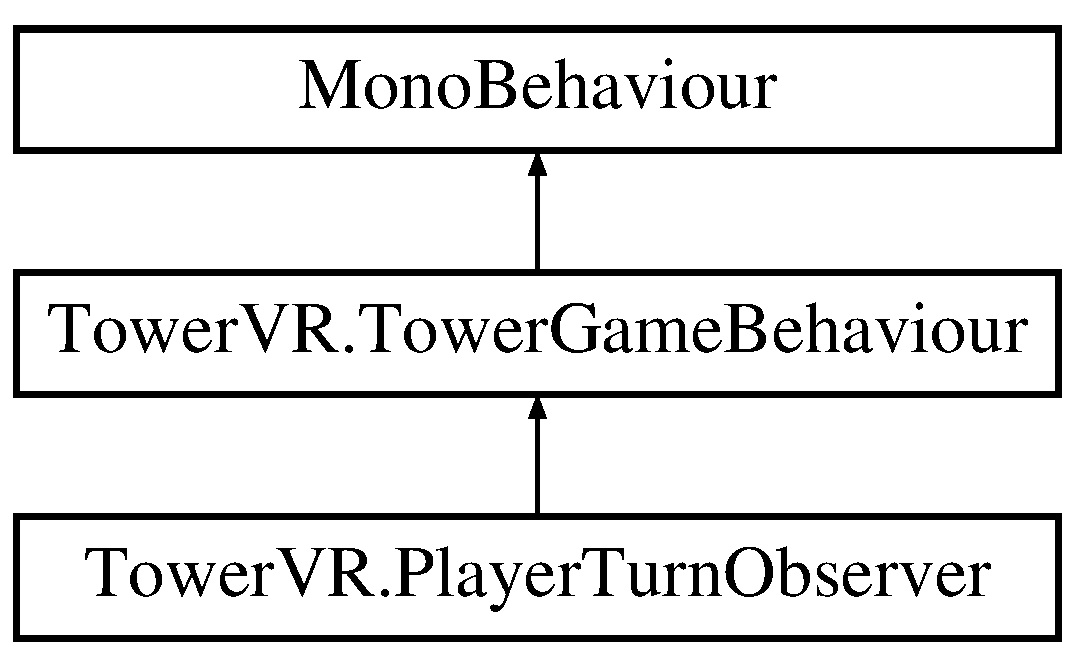
\includegraphics[height=3.000000cm]{class_tower_v_r_1_1_player_turn_observer}
\end{center}
\end{figure}
\subsection*{Additional Inherited Members}


The documentation for this class was generated from the following file\+:\begin{DoxyCompactItemize}
\item 
/\+Users/benjamin/\+Programmering/\+Android\+H\+M\+D/\+Tower\+V\+R/\+Assets/\+Scripts/\+Custom/\+Game/\+\_\+test/Player\+Turn\+Observer.\+cs\end{DoxyCompactItemize}

\hypertarget{class_tower_v_r_1_1_player_won_event}{}\section{Tower\+V\+R.\+Player\+Won\+Event Class Reference}
\label{class_tower_v_r_1_1_player_won_event}\index{Tower\+V\+R.\+Player\+Won\+Event@{Tower\+V\+R.\+Player\+Won\+Event}}
Inheritance diagram for Tower\+V\+R.\+Player\+Won\+Event\+:\begin{figure}[H]
\begin{center}
\leavevmode
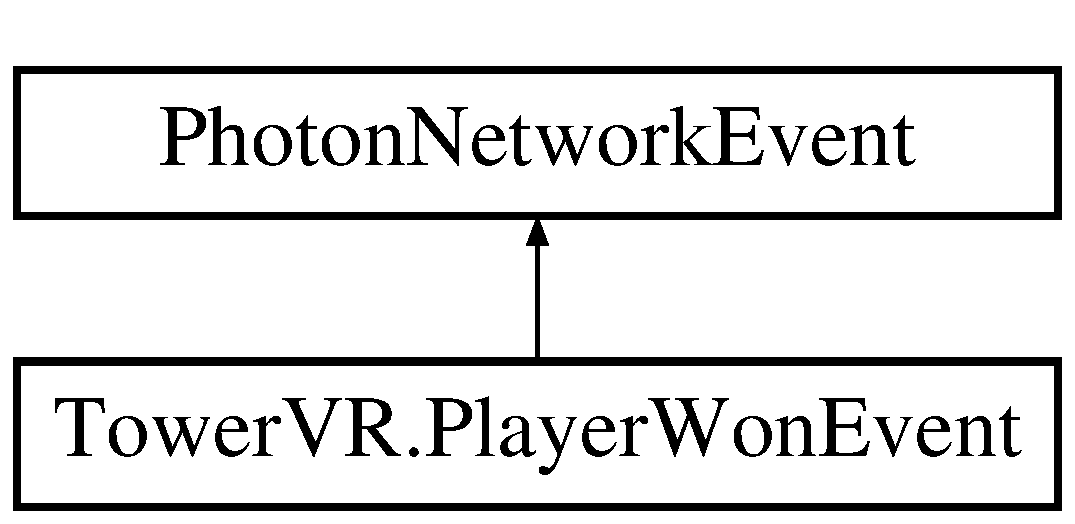
\includegraphics[height=2.000000cm]{class_tower_v_r_1_1_player_won_event}
\end{center}
\end{figure}
\subsection*{Public Member Functions}
\begin{DoxyCompactItemize}
\item 
{\bfseries Player\+Won\+Event} (int player\+ID)\hypertarget{class_tower_v_r_1_1_player_won_event_ab32638f596ec8a7586dce0318a5d3239}{}\label{class_tower_v_r_1_1_player_won_event_ab32638f596ec8a7586dce0318a5d3239}

\end{DoxyCompactItemize}
\subsection*{Static Public Member Functions}
\begin{DoxyCompactItemize}
\item 
static bool \hyperlink{class_tower_v_r_1_1_player_won_event_a97ee6f0bf2f5144573a98fd6eca935f2}{Try\+Parse} (object obj, out int player\+ID)
\end{DoxyCompactItemize}
\subsection*{Additional Inherited Members}


\subsection{Detailed Description}
An event raised when one of the players won the game. 

\subsection{Member Function Documentation}
\index{Tower\+V\+R\+::\+Player\+Won\+Event@{Tower\+V\+R\+::\+Player\+Won\+Event}!Try\+Parse@{Try\+Parse}}
\index{Try\+Parse@{Try\+Parse}!Tower\+V\+R\+::\+Player\+Won\+Event@{Tower\+V\+R\+::\+Player\+Won\+Event}}
\subsubsection[{\texorpdfstring{Try\+Parse(object obj, out int player\+I\+D)}{TryParse(object obj, out int playerID)}}]{\setlength{\rightskip}{0pt plus 5cm}static bool Tower\+V\+R.\+Player\+Won\+Event.\+Try\+Parse (
\begin{DoxyParamCaption}
\item[{object}]{obj, }
\item[{out int}]{player\+ID}
\end{DoxyParamCaption}
)\hspace{0.3cm}{\ttfamily [static]}}\hypertarget{class_tower_v_r_1_1_player_won_event_a97ee6f0bf2f5144573a98fd6eca935f2}{}\label{class_tower_v_r_1_1_player_won_event_a97ee6f0bf2f5144573a98fd6eca935f2}
Tries to parse the contents of the event. 

The documentation for this class was generated from the following file\+:\begin{DoxyCompactItemize}
\item 
/\+Users/benjamin/\+Programmering/\+Android\+H\+M\+D/\+Tower\+V\+R/\+Assets/\+Scripts/\+Custom/\+Game/\+Network/\+Events/Player\+Won\+Event.\+cs\end{DoxyCompactItemize}

\hypertarget{class_randomize_server_name}{}\section{Randomize\+Server\+Name Class Reference}
\label{class_randomize_server_name}\index{Randomize\+Server\+Name@{Randomize\+Server\+Name}}
Inheritance diagram for Randomize\+Server\+Name\+:\begin{figure}[H]
\begin{center}
\leavevmode
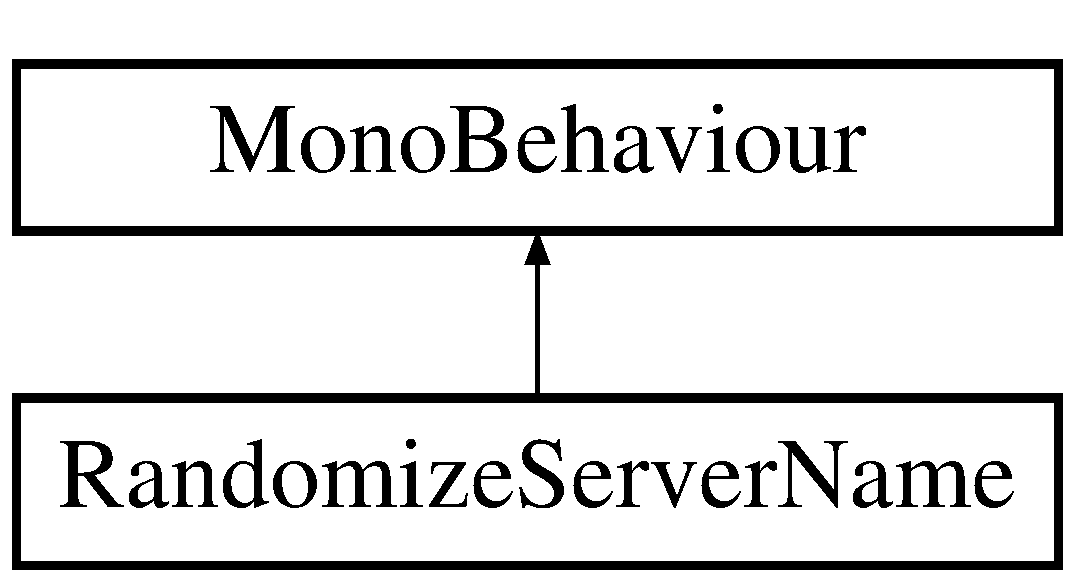
\includegraphics[height=2.000000cm]{class_randomize_server_name}
\end{center}
\end{figure}
\subsection*{Static Public Attributes}
\begin{DoxyCompactItemize}
\item 
static string {\bfseries server\+Name} = \char`\"{}\char`\"{}\hypertarget{class_randomize_server_name_a49311095fceb7d53a264e018f5a5897c}{}\label{class_randomize_server_name_a49311095fceb7d53a264e018f5a5897c}

\end{DoxyCompactItemize}


The documentation for this class was generated from the following file\+:\begin{DoxyCompactItemize}
\item 
/\+Users/benjamin/\+Programmering/\+Android\+H\+M\+D/\+Tower\+V\+R/\+Assets/\+Scripts/\+Custom/\+Game/\+Network/Randomize\+Server\+Name.\+cs\end{DoxyCompactItemize}

\hypertarget{classremove_target_child}{}\section{remove\+Target\+Child Class Reference}
\label{classremove_target_child}\index{remove\+Target\+Child@{remove\+Target\+Child}}
Inheritance diagram for remove\+Target\+Child\+:\begin{figure}[H]
\begin{center}
\leavevmode
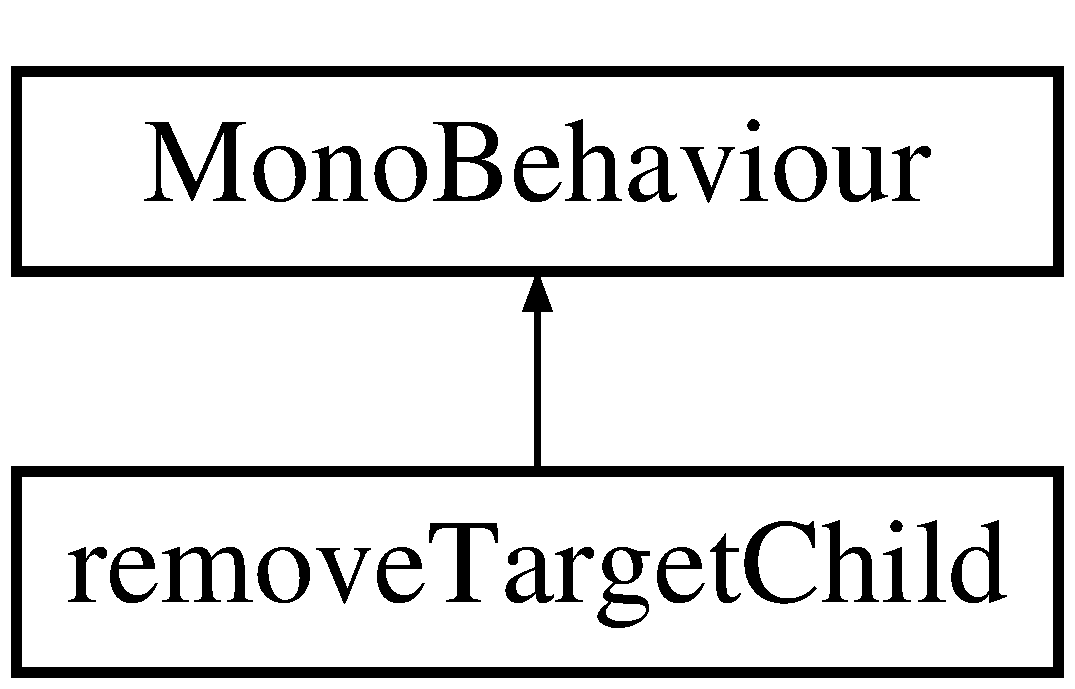
\includegraphics[height=2.000000cm]{classremove_target_child}
\end{center}
\end{figure}


\subsection{Detailed Description}
Removes all sides to the cube so we doesn\textquotesingle{}t render them, or that they occludes objects. 

The documentation for this class was generated from the following file\+:\begin{DoxyCompactItemize}
\item 
/\+Users/benjamin/\+Programmering/\+Android\+H\+M\+D/\+Tower\+V\+R/\+Assets/\+Scripts/\+Custom/\+Generic/remove\+Target\+Child.\+cs\end{DoxyCompactItemize}

\hypertarget{class_restrict_to_host}{}\section{Restrict\+To\+Host Class Reference}
\label{class_restrict_to_host}\index{Restrict\+To\+Host@{Restrict\+To\+Host}}
Inheritance diagram for Restrict\+To\+Host\+:\begin{figure}[H]
\begin{center}
\leavevmode
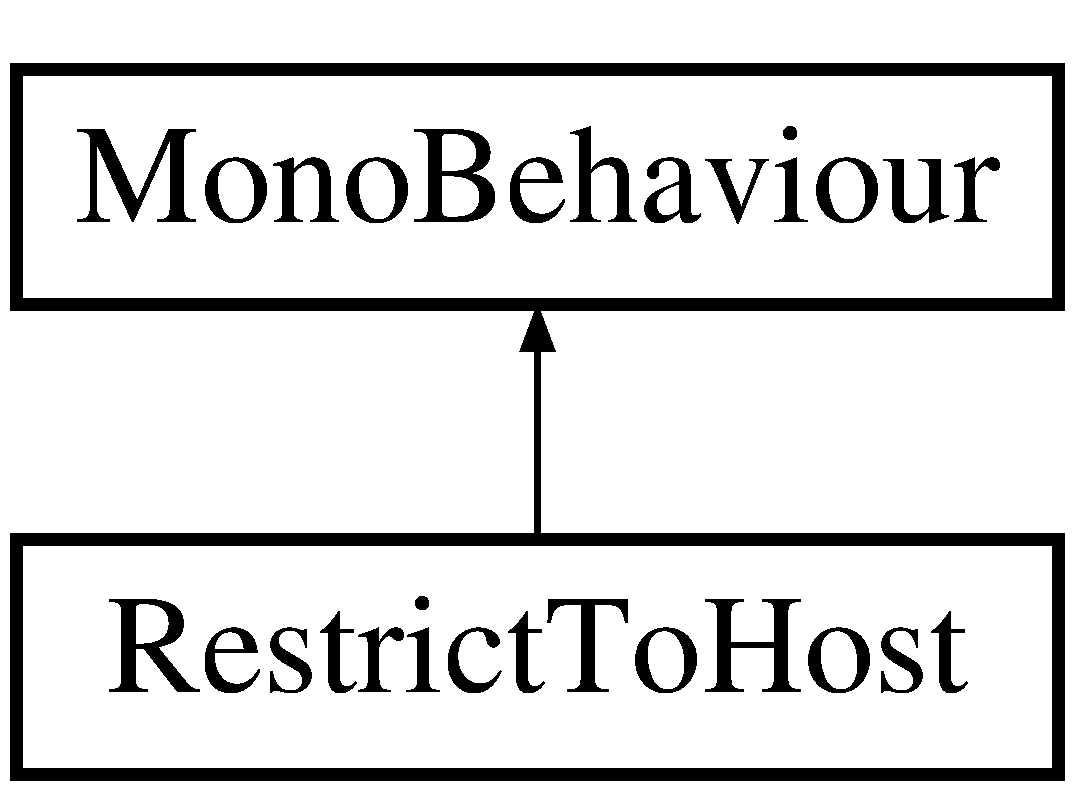
\includegraphics[height=2.000000cm]{class_restrict_to_host}
\end{center}
\end{figure}
\subsection*{Public Attributes}
\begin{DoxyCompactItemize}
\item 
bool {\bfseries debug} = false\hypertarget{class_restrict_to_host_a23cf17fd15f31f44b9dfcbb92f06e495}{}\label{class_restrict_to_host_a23cf17fd15f31f44b9dfcbb92f06e495}

\end{DoxyCompactItemize}


\subsection{Detailed Description}
This script restricts availbility of an object (\char`\"{}this\char`\"{}) to game room host (e.\+g. master according to Photon Unity Networking) 

The documentation for this class was generated from the following file\+:\begin{DoxyCompactItemize}
\item 
/\+Users/benjamin/\+Programmering/\+Android\+H\+M\+D/\+Tower\+V\+R/\+Assets/\+Scripts/\+Custom/\+Game/\+Network/Restrict\+To\+Host.\+cs\end{DoxyCompactItemize}

\hypertarget{class_retrieve_and_spawn_players}{}\section{Retrieve\+And\+Spawn\+Players Class Reference}
\label{class_retrieve_and_spawn_players}\index{Retrieve\+And\+Spawn\+Players@{Retrieve\+And\+Spawn\+Players}}
Inheritance diagram for Retrieve\+And\+Spawn\+Players\+:\begin{figure}[H]
\begin{center}
\leavevmode
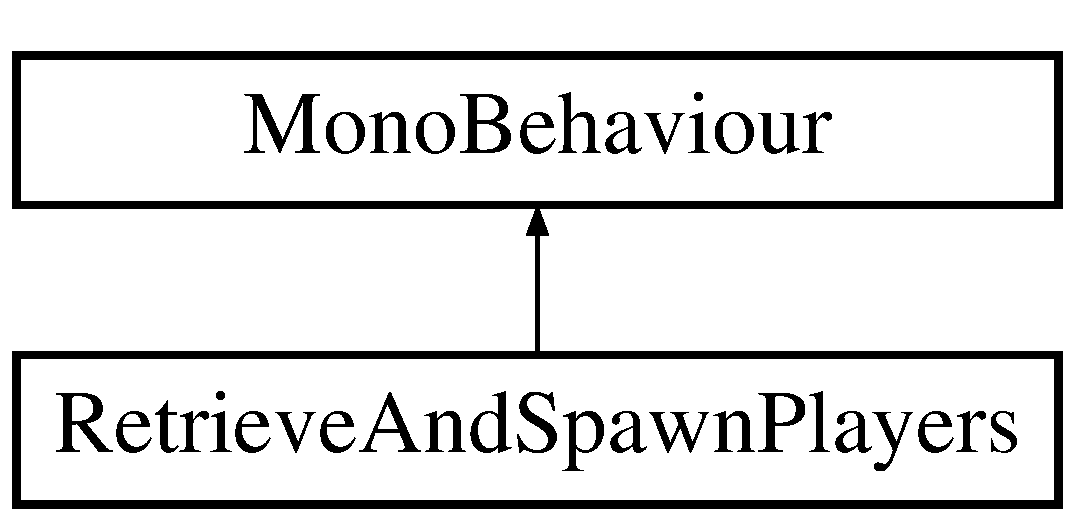
\includegraphics[height=2.000000cm]{class_retrieve_and_spawn_players}
\end{center}
\end{figure}
\subsection*{Public Attributes}
\begin{DoxyCompactItemize}
\item 
string {\bfseries player\+Prefab\+Name}\hypertarget{class_retrieve_and_spawn_players_a91e8dad7d15fe3bb0da9cf4be8b5a5bf}{}\label{class_retrieve_and_spawn_players_a91e8dad7d15fe3bb0da9cf4be8b5a5bf}

\item 
bool {\bfseries debug\+Gui\+On} = false\hypertarget{class_retrieve_and_spawn_players_a5c92cbcb63bda107ecef253968d28f40}{}\label{class_retrieve_and_spawn_players_a5c92cbcb63bda107ecef253968d28f40}

\end{DoxyCompactItemize}


\subsection{Detailed Description}
Retrieves players from active room and spawns them in the scene 

The documentation for this class was generated from the following file\+:\begin{DoxyCompactItemize}
\item 
/\+Users/benjamin/\+Programmering/\+Android\+H\+M\+D/\+Tower\+V\+R/\+Assets/\+Scripts/\+Custom/\+Game/\+Network/Retrieve\+And\+Spawn\+Players.\+cs\end{DoxyCompactItemize}

\hypertarget{class_scene_transition_manager}{}\section{Scene\+Transition\+Manager$<$ T $>$ Class Template Reference}
\label{class_scene_transition_manager}\index{Scene\+Transition\+Manager$<$ T $>$@{Scene\+Transition\+Manager$<$ T $>$}}
Inheritance diagram for Scene\+Transition\+Manager$<$ T $>$\+:\begin{figure}[H]
\begin{center}
\leavevmode
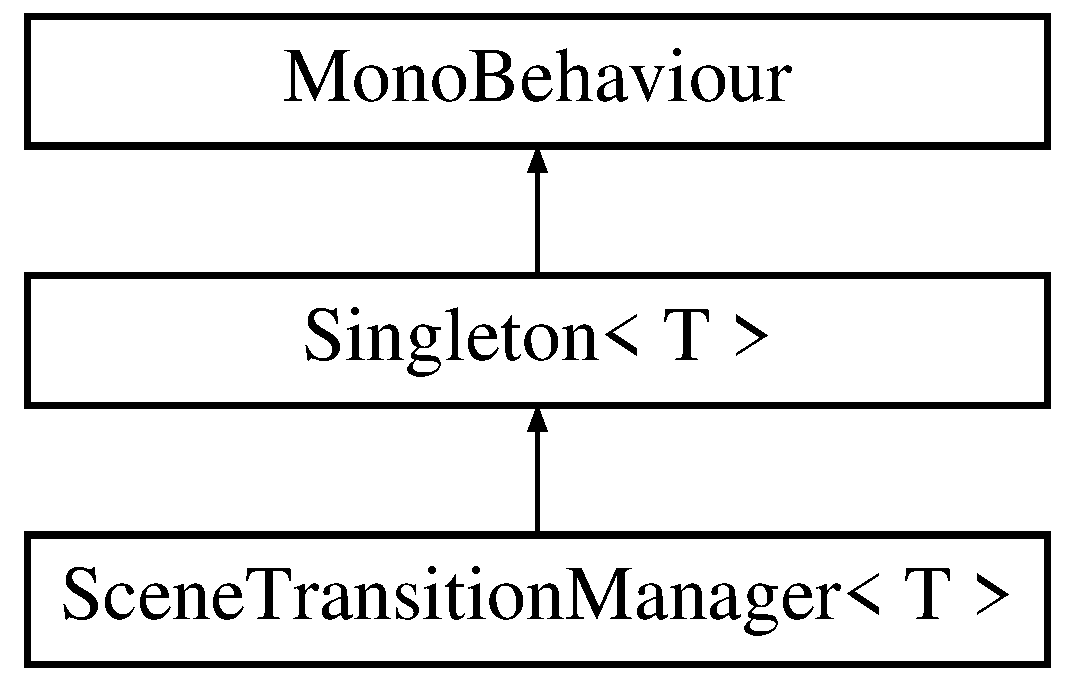
\includegraphics[height=3.000000cm]{class_scene_transition_manager}
\end{center}
\end{figure}
\subsection*{Protected Member Functions}
\begin{DoxyCompactItemize}
\item 
void {\bfseries Load\+Scene} (int scene\+Build\+Index)\hypertarget{class_scene_transition_manager_a1779dbd605c614cf8baf0797f08b3240}{}\label{class_scene_transition_manager_a1779dbd605c614cf8baf0797f08b3240}

\end{DoxyCompactItemize}
\subsection*{Additional Inherited Members}


\subsection{Detailed Description}
A transition manager (singleton) that encapsulates the scene loading behaviour.

Subclasses should expose methods that load specific scenes. \begin{Desc}
\item[Type Constraints]\begin{description}
\item[{\em T} : {\em Mono\+Behaviour}]\end{description}
\end{Desc}


The documentation for this class was generated from the following file\+:\begin{DoxyCompactItemize}
\item 
/\+Users/benjamin/\+Programmering/\+Android\+H\+M\+D/\+Tower\+V\+R/\+Assets/\+Scripts/\+Custom/\+Generic/Scene\+Transition\+Manager.\+cs\end{DoxyCompactItemize}

\hypertarget{struct_tower_v_r_1_1_score}{}\section{Tower\+V\+R.\+Score Struct Reference}
\label{struct_tower_v_r_1_1_score}\index{Tower\+V\+R.\+Score@{Tower\+V\+R.\+Score}}
\subsection*{Public Member Functions}
\begin{DoxyCompactItemize}
\item 
\hyperlink{struct_tower_v_r_1_1_score_afecfe2d8892f0b5c0dce93d4fd4e2356}{Score} (int \hyperlink{struct_tower_v_r_1_1_score_a0c15824361f37b888d650812d162970d}{score})
\end{DoxyCompactItemize}
\subsection*{Static Public Member Functions}
\begin{DoxyCompactItemize}
\item 
static \hyperlink{struct_tower_v_r_1_1_score}{Score} \hyperlink{struct_tower_v_r_1_1_score_aac623a0d5853cf71f1599cdc7dd2f963}{Add} (\hyperlink{struct_tower_v_r_1_1_score}{Score} s1, \hyperlink{struct_tower_v_r_1_1_score}{Score} s2)
\item 
static \hyperlink{struct_tower_v_r_1_1_score}{Score} \hyperlink{struct_tower_v_r_1_1_score_af6094076da2c9cbdab969bf879e4dfcd}{Get\+Score} (Tower\+Piece\+Difficulty tower\+Piece\+Difficulty)
\end{DoxyCompactItemize}
\subsection*{Properties}
\begin{DoxyCompactItemize}
\item 
int \hyperlink{struct_tower_v_r_1_1_score_a0c15824361f37b888d650812d162970d}{score}\hspace{0.3cm}{\ttfamily  \mbox{[}get\mbox{]}}
\end{DoxyCompactItemize}


\subsection{Constructor \& Destructor Documentation}
\index{Tower\+V\+R\+::\+Score@{Tower\+V\+R\+::\+Score}!Score@{Score}}
\index{Score@{Score}!Tower\+V\+R\+::\+Score@{Tower\+V\+R\+::\+Score}}
\subsubsection[{\texorpdfstring{Score(int score)}{Score(int score)}}]{\setlength{\rightskip}{0pt plus 5cm}Tower\+V\+R.\+Score.\+Score (
\begin{DoxyParamCaption}
\item[{int}]{score}
\end{DoxyParamCaption}
)}\hypertarget{struct_tower_v_r_1_1_score_afecfe2d8892f0b5c0dce93d4fd4e2356}{}\label{struct_tower_v_r_1_1_score_afecfe2d8892f0b5c0dce93d4fd4e2356}
Constructs a score object 

\subsection{Member Function Documentation}
\index{Tower\+V\+R\+::\+Score@{Tower\+V\+R\+::\+Score}!Add@{Add}}
\index{Add@{Add}!Tower\+V\+R\+::\+Score@{Tower\+V\+R\+::\+Score}}
\subsubsection[{\texorpdfstring{Add(\+Score s1, Score s2)}{Add(Score s1, Score s2)}}]{\setlength{\rightskip}{0pt plus 5cm}static {\bf Score} Tower\+V\+R.\+Score.\+Add (
\begin{DoxyParamCaption}
\item[{{\bf Score}}]{s1, }
\item[{{\bf Score}}]{s2}
\end{DoxyParamCaption}
)\hspace{0.3cm}{\ttfamily [static]}}\hypertarget{struct_tower_v_r_1_1_score_aac623a0d5853cf71f1599cdc7dd2f963}{}\label{struct_tower_v_r_1_1_score_aac623a0d5853cf71f1599cdc7dd2f963}
Computes the sum of two scores \index{Tower\+V\+R\+::\+Score@{Tower\+V\+R\+::\+Score}!Get\+Score@{Get\+Score}}
\index{Get\+Score@{Get\+Score}!Tower\+V\+R\+::\+Score@{Tower\+V\+R\+::\+Score}}
\subsubsection[{\texorpdfstring{Get\+Score(\+Tower\+Piece\+Difficulty tower\+Piece\+Difficulty)}{GetScore(TowerPieceDifficulty towerPieceDifficulty)}}]{\setlength{\rightskip}{0pt plus 5cm}static {\bf Score} Tower\+V\+R.\+Score.\+Get\+Score (
\begin{DoxyParamCaption}
\item[{Tower\+Piece\+Difficulty}]{tower\+Piece\+Difficulty}
\end{DoxyParamCaption}
)\hspace{0.3cm}{\ttfamily [static]}}\hypertarget{struct_tower_v_r_1_1_score_af6094076da2c9cbdab969bf879e4dfcd}{}\label{struct_tower_v_r_1_1_score_af6094076da2c9cbdab969bf879e4dfcd}
Get the score of a provided difficulty. 

\subsection{Property Documentation}
\index{Tower\+V\+R\+::\+Score@{Tower\+V\+R\+::\+Score}!score@{score}}
\index{score@{score}!Tower\+V\+R\+::\+Score@{Tower\+V\+R\+::\+Score}}
\subsubsection[{\texorpdfstring{score}{score}}]{\setlength{\rightskip}{0pt plus 5cm}int Tower\+V\+R.\+Score.\+score\hspace{0.3cm}{\ttfamily [get]}}\hypertarget{struct_tower_v_r_1_1_score_a0c15824361f37b888d650812d162970d}{}\label{struct_tower_v_r_1_1_score_a0c15824361f37b888d650812d162970d}
The actual score, can only be get not set 

The documentation for this struct was generated from the following file\+:\begin{DoxyCompactItemize}
\item 
/\+Users/benjamin/\+Programmering/\+Android\+H\+M\+D/\+Tower\+V\+R/\+Assets/\+Scripts/\+Custom/\+Game/\+Tower/Score.\+cs\end{DoxyCompactItemize}

\hypertarget{class_tower_v_r_1_1_score_changed_event}{}\section{Tower\+V\+R.\+Score\+Changed\+Event Class Reference}
\label{class_tower_v_r_1_1_score_changed_event}\index{Tower\+V\+R.\+Score\+Changed\+Event@{Tower\+V\+R.\+Score\+Changed\+Event}}
Inheritance diagram for Tower\+V\+R.\+Score\+Changed\+Event\+:\begin{figure}[H]
\begin{center}
\leavevmode
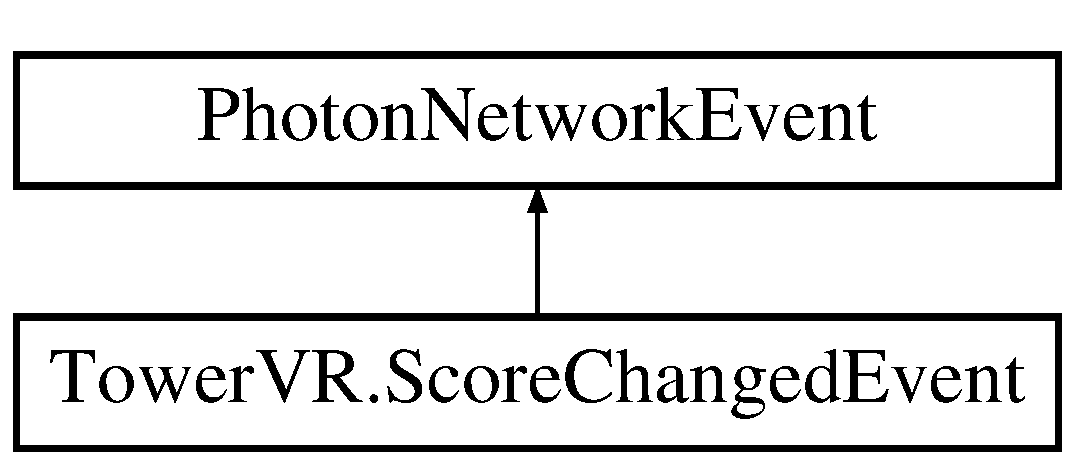
\includegraphics[height=2.000000cm]{class_tower_v_r_1_1_score_changed_event}
\end{center}
\end{figure}
\subsection*{Public Member Functions}
\begin{DoxyCompactItemize}
\item 
{\bfseries Score\+Changed\+Event} (int player\+ID, \hyperlink{struct_tower_v_r_1_1_score}{Score} new\+Score)\hypertarget{class_tower_v_r_1_1_score_changed_event_aff763c9b3f5d45ebf05a94e2f5d5abdb}{}\label{class_tower_v_r_1_1_score_changed_event_aff763c9b3f5d45ebf05a94e2f5d5abdb}

\end{DoxyCompactItemize}
\subsection*{Static Public Member Functions}
\begin{DoxyCompactItemize}
\item 
static bool \hyperlink{class_tower_v_r_1_1_score_changed_event_af3691bfe6c230ac7218d6d0723aedc49}{Try\+Parse} (object obj, out int player\+ID, out \hyperlink{struct_tower_v_r_1_1_score}{Score} new\+Score)
\end{DoxyCompactItemize}
\subsection*{Additional Inherited Members}


\subsection{Detailed Description}
An event raised when the game score was updated for a player. 

\subsection{Member Function Documentation}
\index{Tower\+V\+R\+::\+Score\+Changed\+Event@{Tower\+V\+R\+::\+Score\+Changed\+Event}!Try\+Parse@{Try\+Parse}}
\index{Try\+Parse@{Try\+Parse}!Tower\+V\+R\+::\+Score\+Changed\+Event@{Tower\+V\+R\+::\+Score\+Changed\+Event}}
\subsubsection[{\texorpdfstring{Try\+Parse(object obj, out int player\+I\+D, out Score new\+Score)}{TryParse(object obj, out int playerID, out Score newScore)}}]{\setlength{\rightskip}{0pt plus 5cm}static bool Tower\+V\+R.\+Score\+Changed\+Event.\+Try\+Parse (
\begin{DoxyParamCaption}
\item[{object}]{obj, }
\item[{out int}]{player\+ID, }
\item[{out {\bf Score}}]{new\+Score}
\end{DoxyParamCaption}
)\hspace{0.3cm}{\ttfamily [static]}}\hypertarget{class_tower_v_r_1_1_score_changed_event_af3691bfe6c230ac7218d6d0723aedc49}{}\label{class_tower_v_r_1_1_score_changed_event_af3691bfe6c230ac7218d6d0723aedc49}
Tries to parse the contents of the event. 

The documentation for this class was generated from the following file\+:\begin{DoxyCompactItemize}
\item 
/\+Users/benjamin/\+Programmering/\+Android\+H\+M\+D/\+Tower\+V\+R/\+Assets/\+Scripts/\+Custom/\+Game/\+Network/\+Events/Score\+Changed\+Event.\+cs\end{DoxyCompactItemize}

\hypertarget{class_tower_v_r_1_1_select_tower_piece_event}{}\section{Tower\+V\+R.\+Select\+Tower\+Piece\+Event Class Reference}
\label{class_tower_v_r_1_1_select_tower_piece_event}\index{Tower\+V\+R.\+Select\+Tower\+Piece\+Event@{Tower\+V\+R.\+Select\+Tower\+Piece\+Event}}
Inheritance diagram for Tower\+V\+R.\+Select\+Tower\+Piece\+Event\+:\begin{figure}[H]
\begin{center}
\leavevmode
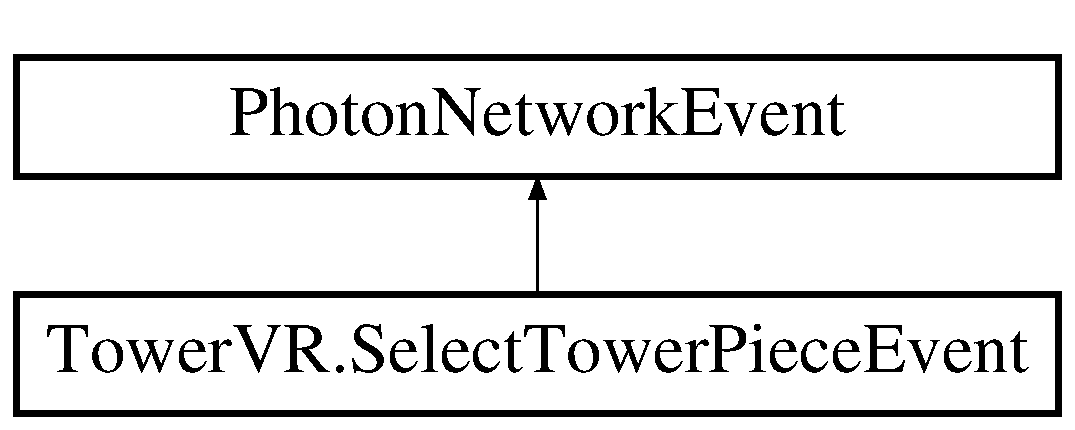
\includegraphics[height=2.000000cm]{class_tower_v_r_1_1_select_tower_piece_event}
\end{center}
\end{figure}
\subsection*{Public Member Functions}
\begin{DoxyCompactItemize}
\item 
{\bfseries Select\+Tower\+Piece\+Event} (Tower\+Piece\+Difficulty difficulty)\hypertarget{class_tower_v_r_1_1_select_tower_piece_event_ad7b86d65e0cd2538fa04f8a23f53ba4a}{}\label{class_tower_v_r_1_1_select_tower_piece_event_ad7b86d65e0cd2538fa04f8a23f53ba4a}

\end{DoxyCompactItemize}
\subsection*{Static Public Member Functions}
\begin{DoxyCompactItemize}
\item 
static bool \hyperlink{class_tower_v_r_1_1_select_tower_piece_event_a104d8aa0fbb14ffc2be371814e18de0c}{Try\+Parse} (object obj, Tower\+Piece\+Difficulty chosen\+Difficulty)
\end{DoxyCompactItemize}
\subsection*{Protected Member Functions}
\begin{DoxyCompactItemize}
\item 
sealed override bool \hyperlink{class_tower_v_r_1_1_select_tower_piece_event_addf1cb68acf541e199df157a32ab25ca}{content\+Is\+Valid} ()
\end{DoxyCompactItemize}
\subsection*{Additional Inherited Members}


\subsection{Detailed Description}
An event sent to the master client when the current player places his/her current tower piece. 

\subsection{Member Function Documentation}
\index{Tower\+V\+R\+::\+Select\+Tower\+Piece\+Event@{Tower\+V\+R\+::\+Select\+Tower\+Piece\+Event}!content\+Is\+Valid@{content\+Is\+Valid}}
\index{content\+Is\+Valid@{content\+Is\+Valid}!Tower\+V\+R\+::\+Select\+Tower\+Piece\+Event@{Tower\+V\+R\+::\+Select\+Tower\+Piece\+Event}}
\subsubsection[{\texorpdfstring{content\+Is\+Valid()}{contentIsValid()}}]{\setlength{\rightskip}{0pt plus 5cm}sealed override bool Tower\+V\+R.\+Select\+Tower\+Piece\+Event.\+content\+Is\+Valid (
\begin{DoxyParamCaption}
{}
\end{DoxyParamCaption}
)\hspace{0.3cm}{\ttfamily [protected]}, {\ttfamily [virtual]}}\hypertarget{class_tower_v_r_1_1_select_tower_piece_event_addf1cb68acf541e199df157a32ab25ca}{}\label{class_tower_v_r_1_1_select_tower_piece_event_addf1cb68acf541e199df157a32ab25ca}
Override this to provide extra content validation. 

Reimplemented from \hyperlink{class_photon_network_event_a82a5487738983085c9e8ac4116474b43}{Photon\+Network\+Event}.

\index{Tower\+V\+R\+::\+Select\+Tower\+Piece\+Event@{Tower\+V\+R\+::\+Select\+Tower\+Piece\+Event}!Try\+Parse@{Try\+Parse}}
\index{Try\+Parse@{Try\+Parse}!Tower\+V\+R\+::\+Select\+Tower\+Piece\+Event@{Tower\+V\+R\+::\+Select\+Tower\+Piece\+Event}}
\subsubsection[{\texorpdfstring{Try\+Parse(object obj, Tower\+Piece\+Difficulty chosen\+Difficulty)}{TryParse(object obj, TowerPieceDifficulty chosenDifficulty)}}]{\setlength{\rightskip}{0pt plus 5cm}static bool Tower\+V\+R.\+Select\+Tower\+Piece\+Event.\+Try\+Parse (
\begin{DoxyParamCaption}
\item[{object}]{obj, }
\item[{Tower\+Piece\+Difficulty}]{chosen\+Difficulty}
\end{DoxyParamCaption}
)\hspace{0.3cm}{\ttfamily [static]}}\hypertarget{class_tower_v_r_1_1_select_tower_piece_event_a104d8aa0fbb14ffc2be371814e18de0c}{}\label{class_tower_v_r_1_1_select_tower_piece_event_a104d8aa0fbb14ffc2be371814e18de0c}
Tries to parse the contents of the event. 

The documentation for this class was generated from the following file\+:\begin{DoxyCompactItemize}
\item 
/\+Users/benjamin/\+Programmering/\+Android\+H\+M\+D/\+Tower\+V\+R/\+Assets/\+Scripts/\+Custom/\+Game/\+Network/\+Events/Select\+Tower\+Piece\+Event.\+cs\end{DoxyCompactItemize}

\hypertarget{class_set_max_players}{}\section{Set\+Max\+Players Class Reference}
\label{class_set_max_players}\index{Set\+Max\+Players@{Set\+Max\+Players}}
Inheritance diagram for Set\+Max\+Players\+:\begin{figure}[H]
\begin{center}
\leavevmode
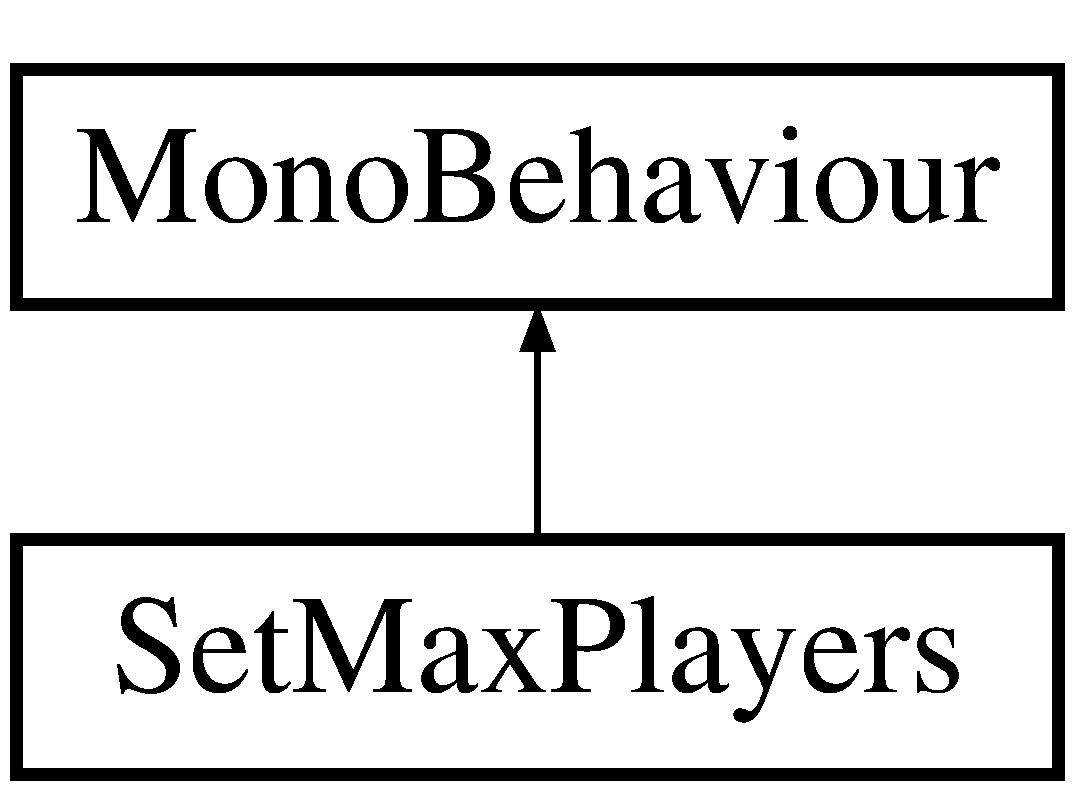
\includegraphics[height=2.000000cm]{class_set_max_players}
\end{center}
\end{figure}
\subsection*{Public Member Functions}
\begin{DoxyCompactItemize}
\item 
void {\bfseries set\+Active} ()\hypertarget{class_set_max_players_afebc031cc7036b36ae05dffe21a32849}{}\label{class_set_max_players_afebc031cc7036b36ae05dffe21a32849}

\end{DoxyCompactItemize}
\subsection*{Public Attributes}
\begin{DoxyCompactItemize}
\item 
int {\bfseries players}\hypertarget{class_set_max_players_a5fee95595f6b72090b66fab053845dd3}{}\label{class_set_max_players_a5fee95595f6b72090b66fab053845dd3}

\end{DoxyCompactItemize}
\subsection*{Static Public Attributes}
\begin{DoxyCompactItemize}
\item 
static int {\bfseries max\+Players} = 0\hypertarget{class_set_max_players_a057c086cee6f48c72f8c042bc267317f}{}\label{class_set_max_players_a057c086cee6f48c72f8c042bc267317f}

\end{DoxyCompactItemize}


The documentation for this class was generated from the following file\+:\begin{DoxyCompactItemize}
\item 
/\+Users/benjamin/\+Programmering/\+Android\+H\+M\+D/\+Tower\+V\+R/\+Assets/\+Scripts/\+Custom/\+Game/\+Network/Set\+Max\+Players.\+cs\end{DoxyCompactItemize}

\hypertarget{class_show_servers}{}\section{Show\+Servers Class Reference}
\label{class_show_servers}\index{Show\+Servers@{Show\+Servers}}
Inheritance diagram for Show\+Servers\+:\begin{figure}[H]
\begin{center}
\leavevmode
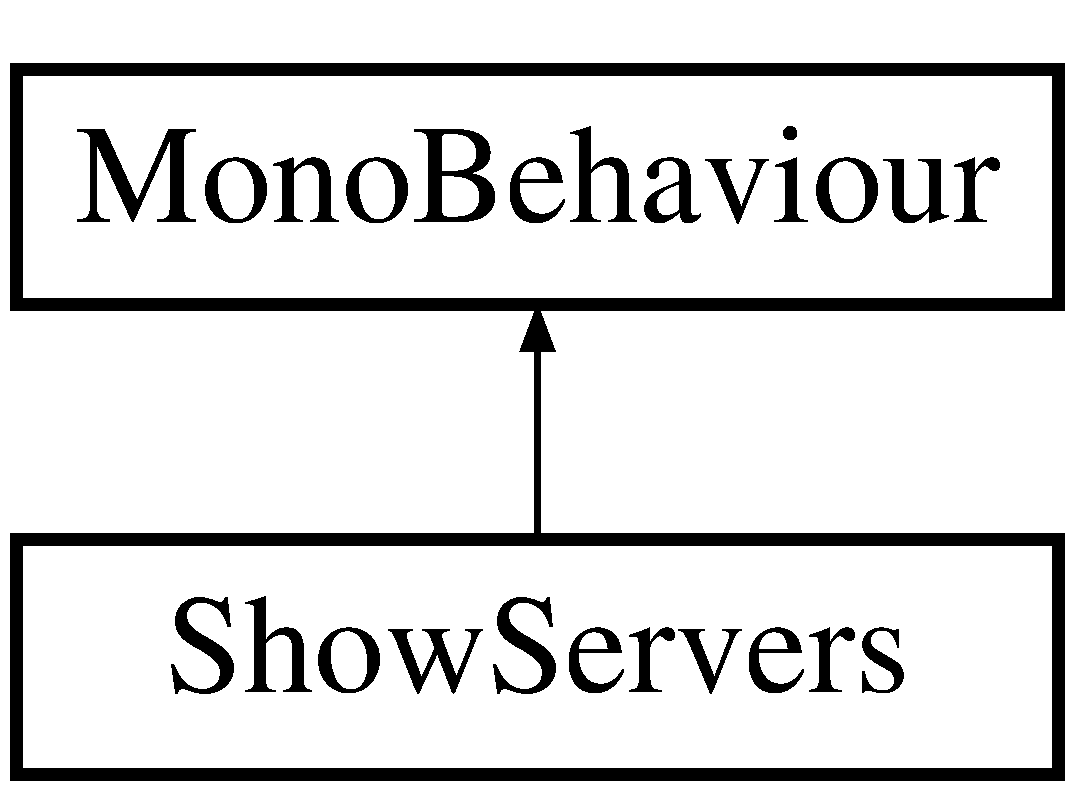
\includegraphics[height=2.000000cm]{class_show_servers}
\end{center}
\end{figure}
\subsection*{Public Member Functions}
\begin{DoxyCompactItemize}
\item 
void {\bfseries On\+Connected\+To\+Master} ()\hypertarget{class_show_servers_a42a7450772bbf1ae31bf576dcf6322d3}{}\label{class_show_servers_a42a7450772bbf1ae31bf576dcf6322d3}

\item 
void {\bfseries Spawn\+Cube} ()\hypertarget{class_show_servers_a69fabbb10d9ea266b32d767a0905ed25}{}\label{class_show_servers_a69fabbb10d9ea266b32d767a0905ed25}

\end{DoxyCompactItemize}
\subsection*{Public Attributes}
\begin{DoxyCompactItemize}
\item 
Game\+Object {\bfseries cube\+Prefab}\hypertarget{class_show_servers_ab9d074dfd7020e70dade8682a7ac69bf}{}\label{class_show_servers_ab9d074dfd7020e70dade8682a7ac69bf}

\end{DoxyCompactItemize}


The documentation for this class was generated from the following file\+:\begin{DoxyCompactItemize}
\item 
/\+Users/benjamin/\+Programmering/\+Android\+H\+M\+D/\+Tower\+V\+R/\+Assets/\+Scripts/\+Custom/\+Game/\+Network/Show\+Servers.\+cs\end{DoxyCompactItemize}

\hypertarget{class_singleton}{}\section{Singleton$<$ T $>$ Class Template Reference}
\label{class_singleton}\index{Singleton$<$ T $>$@{Singleton$<$ T $>$}}
Inheritance diagram for Singleton$<$ T $>$\+:\begin{figure}[H]
\begin{center}
\leavevmode
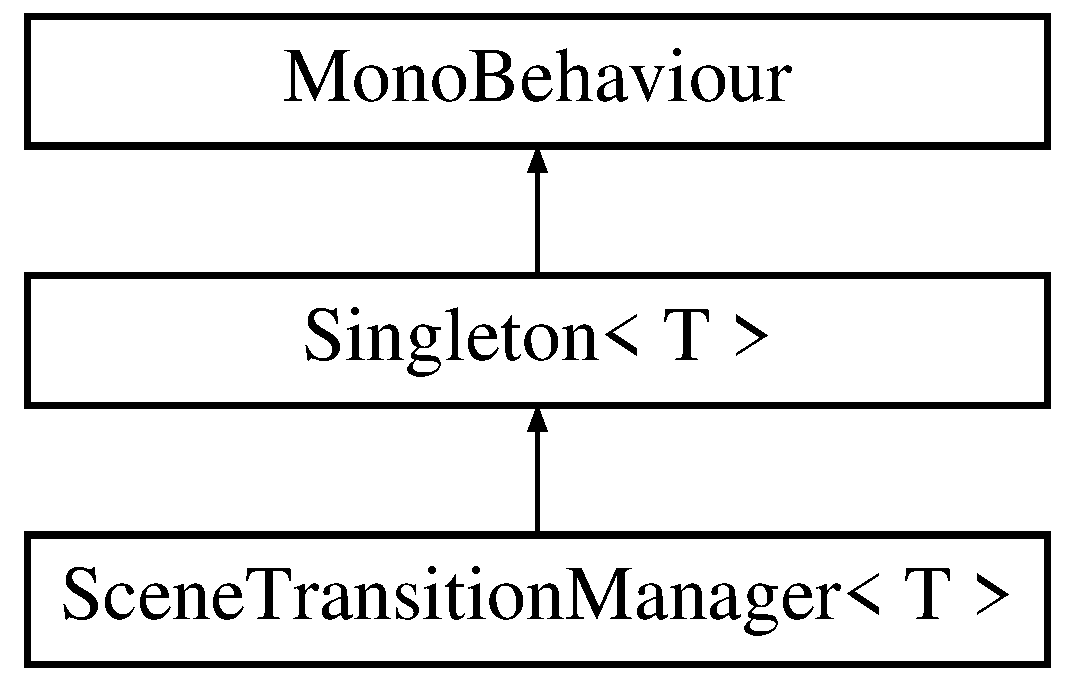
\includegraphics[height=3.000000cm]{class_singleton}
\end{center}
\end{figure}
\subsection*{Static Protected Attributes}
\begin{DoxyCompactItemize}
\item 
static T {\bfseries instance}\hypertarget{class_singleton_ac160511cdbe3795f209bfdd1874dcacd}{}\label{class_singleton_ac160511cdbe3795f209bfdd1874dcacd}

\end{DoxyCompactItemize}
\subsection*{Properties}
\begin{DoxyCompactItemize}
\item 
static T \hyperlink{class_singleton_a54103e8475b2a352ee759d5732307534}{Instance}\hspace{0.3cm}{\ttfamily  \mbox{[}get\mbox{]}}
\end{DoxyCompactItemize}


\subsection{Detailed Description}
\hyperlink{class_singleton}{Singleton} is a design pattern for ensuring that a class only ever has a single instance. Each class that inherits from this abstract base class will automatically be a singleton, given that an instance of the class is attached to a Game\+Object.

The singleton instance is retrieved by calling \char`\"{}\+Class\+Name\char`\"{}.Instance \begin{Desc}
\item[Type Constraints]\begin{description}
\item[{\em T} : {\em Mono\+Behaviour}]\end{description}
\end{Desc}


\subsection{Property Documentation}
\index{Singleton@{Singleton}!Instance@{Instance}}
\index{Instance@{Instance}!Singleton@{Singleton}}
\subsubsection[{\texorpdfstring{Instance}{Instance}}]{\setlength{\rightskip}{0pt plus 5cm}T {\bf Singleton}$<$ T $>$.Instance\hspace{0.3cm}{\ttfamily [static]}, {\ttfamily [get]}}\hypertarget{class_singleton_a54103e8475b2a352ee759d5732307534}{}\label{class_singleton_a54103e8475b2a352ee759d5732307534}
Returns the instance of this singleton 

The documentation for this class was generated from the following file\+:\begin{DoxyCompactItemize}
\item 
/\+Users/benjamin/\+Programmering/\+Android\+H\+M\+D/\+Tower\+V\+R/\+Assets/\+Scripts/\+Custom/\+Generic/Singleton.\+cs\end{DoxyCompactItemize}

\hypertarget{class_spawn_selected_level}{}\section{Spawn\+Selected\+Level Class Reference}
\label{class_spawn_selected_level}\index{Spawn\+Selected\+Level@{Spawn\+Selected\+Level}}
Inheritance diagram for Spawn\+Selected\+Level\+:\begin{figure}[H]
\begin{center}
\leavevmode
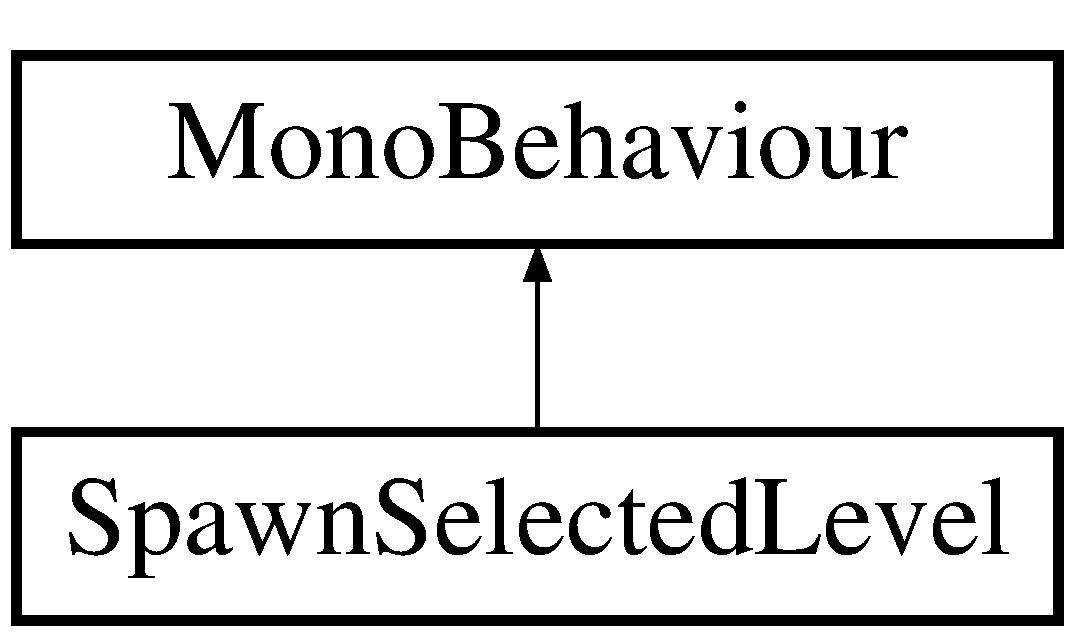
\includegraphics[height=2.000000cm]{class_spawn_selected_level}
\end{center}
\end{figure}
\subsection*{Public Attributes}
\begin{DoxyCompactItemize}
\item 
Game\+Object {\bfseries Level\+Components}\hypertarget{class_spawn_selected_level_a604f58d67bb353137f526689fecd1738}{}\label{class_spawn_selected_level_a604f58d67bb353137f526689fecd1738}

\item 
Material {\bfseries Material1}\hypertarget{class_spawn_selected_level_a366848fc78a8c064b11ca751d3d6025a}{}\label{class_spawn_selected_level_a366848fc78a8c064b11ca751d3d6025a}

\item 
Material {\bfseries Skybox}\hypertarget{class_spawn_selected_level_a13d055e319c08c9e52f37d8b810889f0}{}\label{class_spawn_selected_level_a13d055e319c08c9e52f37d8b810889f0}

\end{DoxyCompactItemize}
\subsection*{Static Public Attributes}
\begin{DoxyCompactItemize}
\item 
static string \hyperlink{class_spawn_selected_level_a8d218aa712c1464b1e6a928e52cdb56f}{Loaded\+Level}
\item 
static string {\bfseries Loaded\+Material1}\hypertarget{class_spawn_selected_level_a47b76272906237a6f5eb652908cebda6}{}\label{class_spawn_selected_level_a47b76272906237a6f5eb652908cebda6}

\item 
static string {\bfseries Loaded\+Skybox}\hypertarget{class_spawn_selected_level_a572973e025315254b42897c1bf2d5f3e}{}\label{class_spawn_selected_level_a572973e025315254b42897c1bf2d5f3e}

\end{DoxyCompactItemize}


\subsection{Member Data Documentation}
\index{Spawn\+Selected\+Level@{Spawn\+Selected\+Level}!Loaded\+Level@{Loaded\+Level}}
\index{Loaded\+Level@{Loaded\+Level}!Spawn\+Selected\+Level@{Spawn\+Selected\+Level}}
\subsubsection[{\texorpdfstring{Loaded\+Level}{LoadedLevel}}]{\setlength{\rightskip}{0pt plus 5cm}string Spawn\+Selected\+Level.\+Loaded\+Level\hspace{0.3cm}{\ttfamily [static]}}\hypertarget{class_spawn_selected_level_a8d218aa712c1464b1e6a928e52cdb56f}{}\label{class_spawn_selected_level_a8d218aa712c1464b1e6a928e52cdb56f}
Assume the level selection scene is \char`\"{}\+Scene 0\char`\"{} and the game scene is \char`\"{}\+Scene 1\char`\"{}.

Add this script to the scene manager in the game scene. (Scene 1) This scripts needs info form another script on the level-\/selection object ( in Scene 0). The public static string variables in this scripts should be assigned when clicking the level-\/selection object (in another script in scene 0). -\/\+EX\+: On\+Click()\{\hyperlink{class_spawn_selected_level_a8d218aa712c1464b1e6a928e52cdb56f}{Spawn\+Selected\+Level.\+Loaded\+Level} = Level\+Name;\} //\+When clicking (selecting the level), set the name of the prefab level to load.

See example in the script \char`\"{}\+Mouse\+Over.\+cs\char`\"{} in the Unity/\+Scripts folder (Google Drive).

O\+BS\+: Remember to destroy objects when leaving the scene. 

The documentation for this class was generated from the following file\+:\begin{DoxyCompactItemize}
\item 
/\+Users/benjamin/\+Programmering/\+Android\+H\+M\+D/\+Tower\+V\+R/\+Assets/\+Scripts/\+Custom/Spawn\+Selected\+Level.\+cs\end{DoxyCompactItemize}

\hypertarget{class_timer}{}\section{Timer Class Reference}
\label{class_timer}\index{Timer@{Timer}}
Inheritance diagram for Timer\+:\begin{figure}[H]
\begin{center}
\leavevmode
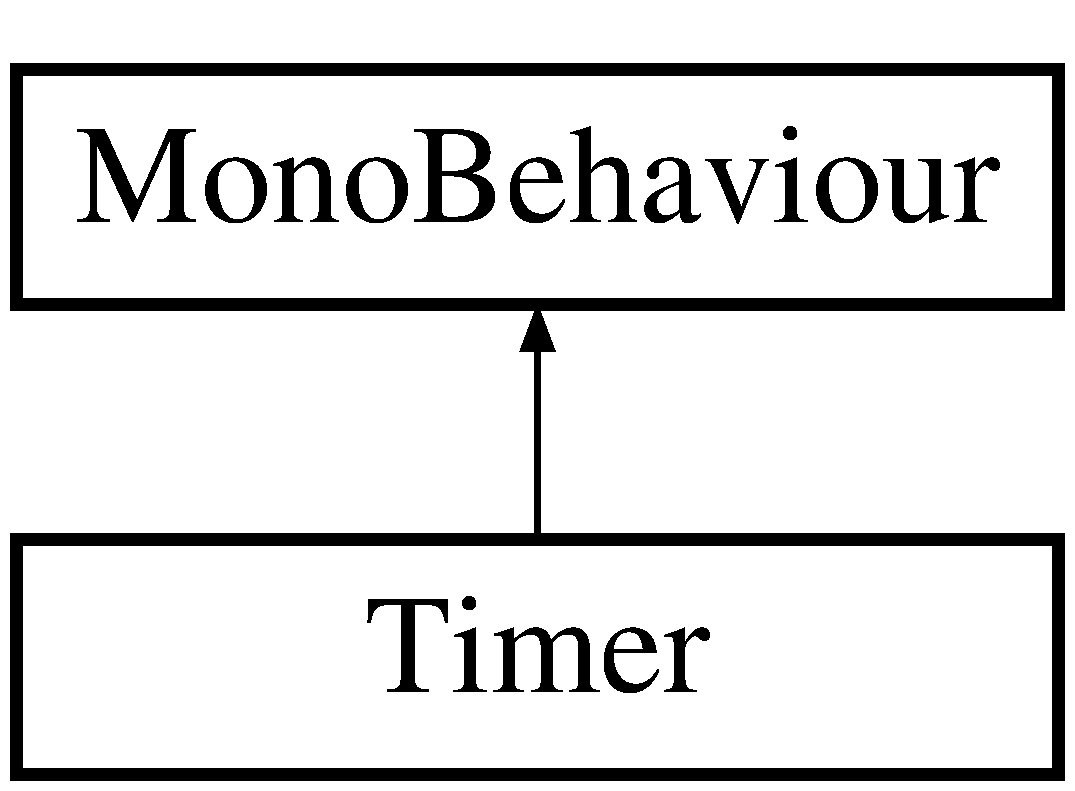
\includegraphics[height=2.000000cm]{class_timer}
\end{center}
\end{figure}
\subsection*{Public Member Functions}
\begin{DoxyCompactItemize}
\item 
double \hyperlink{class_timer_a503e3079434bb29dea47df85b1054df2}{start} ()
\item 
double \hyperlink{class_timer_a113c5465a77c4ea4be43cf45b97260fb}{stop} ()
\item 
double \hyperlink{class_timer_a328e44f5e5328d870080142a823229a0}{clear} ()
\end{DoxyCompactItemize}
\subsection*{Properties}
\begin{DoxyCompactItemize}
\item 
double \hyperlink{class_timer_a0651beb618585fa536c07e38163dc24b}{time}\hspace{0.3cm}{\ttfamily  \mbox{[}get\mbox{]}}
\end{DoxyCompactItemize}


\subsection{Detailed Description}
Simple timer class. Is a Unity component that automatically updates its internal timer. 

\subsection{Member Function Documentation}
\index{Timer@{Timer}!clear@{clear}}
\index{clear@{clear}!Timer@{Timer}}
\subsubsection[{\texorpdfstring{clear()}{clear()}}]{\setlength{\rightskip}{0pt plus 5cm}double Timer.\+clear (
\begin{DoxyParamCaption}
{}
\end{DoxyParamCaption}
)}\hypertarget{class_timer_a328e44f5e5328d870080142a823229a0}{}\label{class_timer_a328e44f5e5328d870080142a823229a0}
Clears the timer. Returns the timer count before setting it to zero. \index{Timer@{Timer}!start@{start}}
\index{start@{start}!Timer@{Timer}}
\subsubsection[{\texorpdfstring{start()}{start()}}]{\setlength{\rightskip}{0pt plus 5cm}double Timer.\+start (
\begin{DoxyParamCaption}
{}
\end{DoxyParamCaption}
)}\hypertarget{class_timer_a503e3079434bb29dea47df85b1054df2}{}\label{class_timer_a503e3079434bb29dea47df85b1054df2}
Start the timer. Returns its current timer count. \index{Timer@{Timer}!stop@{stop}}
\index{stop@{stop}!Timer@{Timer}}
\subsubsection[{\texorpdfstring{stop()}{stop()}}]{\setlength{\rightskip}{0pt plus 5cm}double Timer.\+stop (
\begin{DoxyParamCaption}
{}
\end{DoxyParamCaption}
)}\hypertarget{class_timer_a113c5465a77c4ea4be43cf45b97260fb}{}\label{class_timer_a113c5465a77c4ea4be43cf45b97260fb}
Stops the timer. Returns its current timer count. 

\subsection{Property Documentation}
\index{Timer@{Timer}!time@{time}}
\index{time@{time}!Timer@{Timer}}
\subsubsection[{\texorpdfstring{time}{time}}]{\setlength{\rightskip}{0pt plus 5cm}double Timer.\+time\hspace{0.3cm}{\ttfamily [get]}}\hypertarget{class_timer_a0651beb618585fa536c07e38163dc24b}{}\label{class_timer_a0651beb618585fa536c07e38163dc24b}
The timer\textquotesingle{}s value, in seconds. 

The documentation for this class was generated from the following file\+:\begin{DoxyCompactItemize}
\item 
/\+Users/benjamin/\+Programmering/\+Android\+H\+M\+D/\+Tower\+V\+R/\+Assets/\+Scripts/\+Custom/\+Generic/Timer.\+cs\end{DoxyCompactItemize}

\hypertarget{class_torus}{}\section{Torus Class Reference}
\label{class_torus}\index{Torus@{Torus}}
Inheritance diagram for Torus\+:\begin{figure}[H]
\begin{center}
\leavevmode
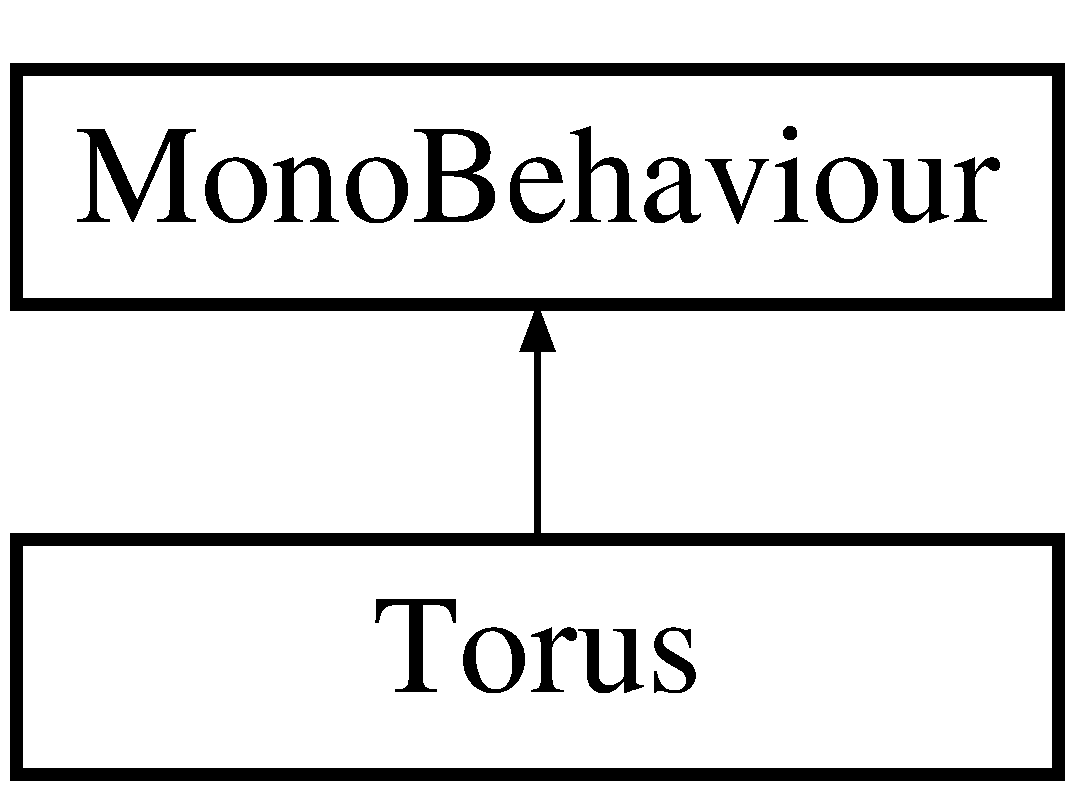
\includegraphics[height=2.000000cm]{class_torus}
\end{center}
\end{figure}
\subsection*{Public Member Functions}
\begin{DoxyCompactItemize}
\item 
void {\bfseries Refresh\+Torus} ()\hypertarget{class_torus_a11488676c74af823a124085c3af72aa3}{}\label{class_torus_a11488676c74af823a124085c3af72aa3}

\end{DoxyCompactItemize}
\subsection*{Public Attributes}
\begin{DoxyCompactItemize}
\item 
float {\bfseries segment\+Radius} = 1f\hypertarget{class_torus_a8dd1e53cd1fb9415fbe64b7004ba274c}{}\label{class_torus_a8dd1e53cd1fb9415fbe64b7004ba274c}

\item 
float {\bfseries tube\+Radius} = 0.\+1f\hypertarget{class_torus_af176474a9c7b704f10c2fd58b33771f8}{}\label{class_torus_af176474a9c7b704f10c2fd58b33771f8}

\item 
int {\bfseries num\+Segments} = 32\hypertarget{class_torus_a5c0c35544de72aa99edaa76d5b7357d8}{}\label{class_torus_a5c0c35544de72aa99edaa76d5b7357d8}

\item 
int {\bfseries num\+Tubes} = 12\hypertarget{class_torus_a7f981e7fbdfedb7170aba45013673dff}{}\label{class_torus_a7f981e7fbdfedb7170aba45013673dff}

\end{DoxyCompactItemize}


The documentation for this class was generated from the following file\+:\begin{DoxyCompactItemize}
\item 
/\+Users/benjamin/\+Programmering/\+Android\+H\+M\+D/\+Tower\+V\+R/\+Assets/\+Scripts/\+Custom/Torus.\+cs\end{DoxyCompactItemize}

\hypertarget{class_torus_generator}{}\section{Torus\+Generator Class Reference}
\label{class_torus_generator}\index{Torus\+Generator@{Torus\+Generator}}
Inheritance diagram for Torus\+Generator\+:\begin{figure}[H]
\begin{center}
\leavevmode
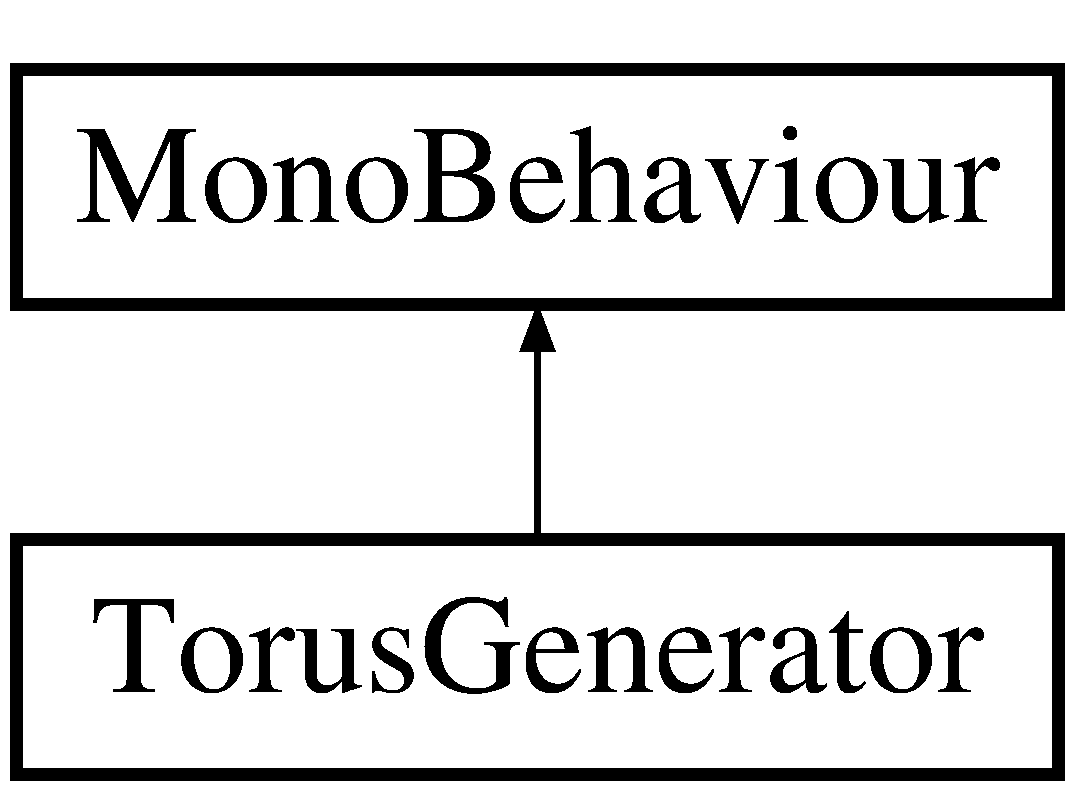
\includegraphics[height=2.000000cm]{class_torus_generator}
\end{center}
\end{figure}
\subsection*{Public Member Functions}
\begin{DoxyCompactItemize}
\item 
void {\bfseries torus} (Game\+Object torus\+Mesh, float segment\+Radius, float tube\+Radius, int num\+Segments, int num\+Tubes)\hypertarget{class_torus_generator_ace97cc7d5209d135b935407b7a554f50}{}\label{class_torus_generator_ace97cc7d5209d135b935407b7a554f50}

\end{DoxyCompactItemize}
\subsection*{Public Attributes}
\begin{DoxyCompactItemize}
\item 
float {\bfseries segment\+Radius} = 1f\hypertarget{class_torus_generator_aed33038eb45157a8feff1e38d07c09bb}{}\label{class_torus_generator_aed33038eb45157a8feff1e38d07c09bb}

\item 
float {\bfseries tube\+Radius} = 0.\+1f\hypertarget{class_torus_generator_a7cbc4daec94ddb0bfbbb2740eb19932c}{}\label{class_torus_generator_a7cbc4daec94ddb0bfbbb2740eb19932c}

\item 
int {\bfseries num\+Segments} = 32\hypertarget{class_torus_generator_ad259d2293d49c58c1ab23418cae7d462}{}\label{class_torus_generator_ad259d2293d49c58c1ab23418cae7d462}

\item 
int {\bfseries num\+Tubes} = 12\hypertarget{class_torus_generator_a7dbdd0f36b47f20ebdf8f235c1d3d27e}{}\label{class_torus_generator_a7dbdd0f36b47f20ebdf8f235c1d3d27e}

\item 
string {\bfseries torus\+Game\+Object\+Name} = \char`\"{}Torus\+Mesh\char`\"{}\hypertarget{class_torus_generator_a0be1daa18ad5c4aa772471ded8e65dbe}{}\label{class_torus_generator_a0be1daa18ad5c4aa772471ded8e65dbe}

\item 
Color {\bfseries color} = Color.\+blue\hypertarget{class_torus_generator_aa8bebfe24d304aa83881e1e676d3fa35}{}\label{class_torus_generator_aa8bebfe24d304aa83881e1e676d3fa35}

\end{DoxyCompactItemize}


The documentation for this class was generated from the following file\+:\begin{DoxyCompactItemize}
\item 
/\+Users/benjamin/\+Programmering/\+Android\+H\+M\+D/\+Tower\+V\+R/\+Assets/\+Scripts/\+Custom/Torus\+Generator.\+cs\end{DoxyCompactItemize}

\hypertarget{class_tower_v_r_1_1_tower_game_behaviour}{}\section{Tower\+V\+R.\+Tower\+Game\+Behaviour Class Reference}
\label{class_tower_v_r_1_1_tower_game_behaviour}\index{Tower\+V\+R.\+Tower\+Game\+Behaviour@{Tower\+V\+R.\+Tower\+Game\+Behaviour}}
Inheritance diagram for Tower\+V\+R.\+Tower\+Game\+Behaviour\+:\begin{figure}[H]
\begin{center}
\leavevmode
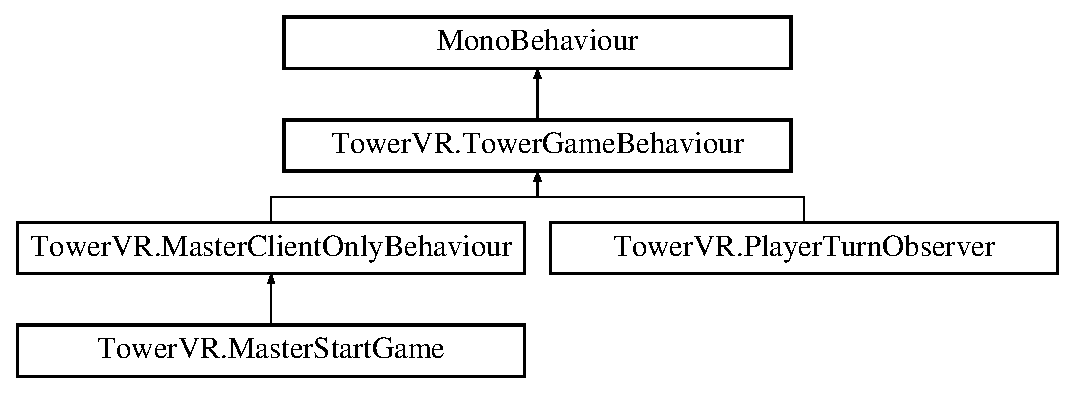
\includegraphics[height=4.000000cm]{class_tower_v_r_1_1_tower_game_behaviour}
\end{center}
\end{figure}
\subsection*{Properties}
\begin{DoxyCompactItemize}
\item 
\hyperlink{class_tower_v_r_1_1_tower_game_manager}{Tower\+Game\+Manager} \hyperlink{class_tower_v_r_1_1_tower_game_behaviour_a5f0dc5fad7fbdcd09370d373329c00c7}{manager}\hspace{0.3cm}{\ttfamily  \mbox{[}get\mbox{]}}
\end{DoxyCompactItemize}


\subsection{Detailed Description}
Base Behaviour class that provides convenience access to the scene\textquotesingle{}s \hyperlink{class_tower_v_r_1_1_tower_game_manager}{Tower\+Game\+Manager}.

Refer to the \hyperlink{class_tower_v_r_1_1_tower_game_manager}{Tower\+Game\+Manager}\textquotesingle{}s \char`\"{}\+D\+E\+L\+E\+G\+A\+T\+E\+S\char`\"{}-\/documentation to see usage. 

\subsection{Property Documentation}
\index{Tower\+V\+R\+::\+Tower\+Game\+Behaviour@{Tower\+V\+R\+::\+Tower\+Game\+Behaviour}!manager@{manager}}
\index{manager@{manager}!Tower\+V\+R\+::\+Tower\+Game\+Behaviour@{Tower\+V\+R\+::\+Tower\+Game\+Behaviour}}
\subsubsection[{\texorpdfstring{manager}{manager}}]{\setlength{\rightskip}{0pt plus 5cm}{\bf Tower\+Game\+Manager} Tower\+V\+R.\+Tower\+Game\+Behaviour.\+manager\hspace{0.3cm}{\ttfamily [get]}, {\ttfamily [protected]}}\hypertarget{class_tower_v_r_1_1_tower_game_behaviour_a5f0dc5fad7fbdcd09370d373329c00c7}{}\label{class_tower_v_r_1_1_tower_game_behaviour_a5f0dc5fad7fbdcd09370d373329c00c7}
Exposed property that retrieves the scene\textquotesingle{}s \hyperlink{class_tower_v_r_1_1_tower_game_manager}{Tower\+Game\+Manager} singleton instance. 

The documentation for this class was generated from the following file\+:\begin{DoxyCompactItemize}
\item 
/\+Users/benjamin/\+Programmering/\+Android\+H\+M\+D/\+Tower\+V\+R/\+Assets/\+Scripts/\+Custom/\+Game/\+Tower/Tower\+Game\+Behaviour.\+cs\end{DoxyCompactItemize}

\hypertarget{class_tower_v_r_1_1_tower_game_manager}{}\section{Tower\+V\+R.\+Tower\+Game\+Manager Class Reference}
\label{class_tower_v_r_1_1_tower_game_manager}\index{Tower\+V\+R.\+Tower\+Game\+Manager@{Tower\+V\+R.\+Tower\+Game\+Manager}}
Inheritance diagram for Tower\+V\+R.\+Tower\+Game\+Manager\+:\begin{figure}[H]
\begin{center}
\leavevmode
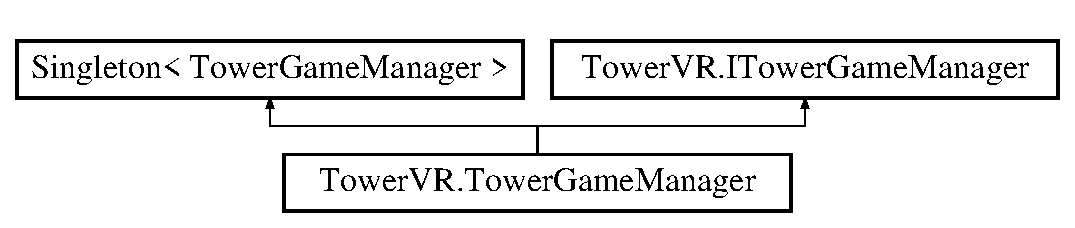
\includegraphics[height=2.000000cm]{class_tower_v_r_1_1_tower_game_manager}
\end{center}
\end{figure}
\subsection*{Public Member Functions}
\begin{DoxyCompactItemize}
\item 
void \hyperlink{class_tower_v_r_1_1_tower_game_manager_a7ea173c143c836423cc25e8f0eed970d}{notify\+Is\+Ready} ()\hypertarget{class_tower_v_r_1_1_tower_game_manager_a7ea173c143c836423cc25e8f0eed970d}{}\label{class_tower_v_r_1_1_tower_game_manager_a7ea173c143c836423cc25e8f0eed970d}

\begin{DoxyCompactList}\small\item\em See \hyperlink{interface_tower_v_r_1_1_i_tower_game_manager}{I\+Tower\+Game\+Manager}. \end{DoxyCompactList}\item 
void \hyperlink{class_tower_v_r_1_1_tower_game_manager_a489f27c61ec3d5c29ac56fea0a024cf6}{try\+Start\+Game} ()\hypertarget{class_tower_v_r_1_1_tower_game_manager_a489f27c61ec3d5c29ac56fea0a024cf6}{}\label{class_tower_v_r_1_1_tower_game_manager_a489f27c61ec3d5c29ac56fea0a024cf6}

\begin{DoxyCompactList}\small\item\em See \hyperlink{interface_tower_v_r_1_1_i_tower_game_manager}{I\+Tower\+Game\+Manager}. \end{DoxyCompactList}\item 
void \hyperlink{class_tower_v_r_1_1_tower_game_manager_aaa476cfb148a19c6579c38823dd37fd3}{place\+Tower\+Piece} (float positionX, float positionZ, float rotation\+DegreesY)\hypertarget{class_tower_v_r_1_1_tower_game_manager_aaa476cfb148a19c6579c38823dd37fd3}{}\label{class_tower_v_r_1_1_tower_game_manager_aaa476cfb148a19c6579c38823dd37fd3}

\begin{DoxyCompactList}\small\item\em See \hyperlink{interface_tower_v_r_1_1_i_tower_game_manager}{I\+Tower\+Game\+Manager}. \end{DoxyCompactList}\item 
delegate void \hyperlink{class_tower_v_r_1_1_tower_game_manager_a4bfd43a7fbaab6c26aa918ff220f11f8}{Game\+State\+Changed\+Handler} (int game\+State)
\item 
delegate void {\bfseries Turn\+State\+Changed\+Handler} (int turn\+State)\hypertarget{class_tower_v_r_1_1_tower_game_manager_aa05ec13ba870bbe24fe436ffe251889e}{}\label{class_tower_v_r_1_1_tower_game_manager_aa05ec13ba870bbe24fe436ffe251889e}

\item 
delegate void {\bfseries Player\+Lost\+Handler} (int losing\+Player\+ID)\hypertarget{class_tower_v_r_1_1_tower_game_manager_a9caa83a7218ba6076cb2b486373bb8dc}{}\label{class_tower_v_r_1_1_tower_game_manager_a9caa83a7218ba6076cb2b486373bb8dc}

\item 
delegate void {\bfseries Player\+Won\+Handler} (int winning\+Player\+ID)\hypertarget{class_tower_v_r_1_1_tower_game_manager_a686d2c9d0920eade95dc5a3156da132c}{}\label{class_tower_v_r_1_1_tower_game_manager_a686d2c9d0920eade95dc5a3156da132c}

\item 
delegate void {\bfseries Next\+Player\+Turn\+Handler} (int next\+Player\+ID)\hypertarget{class_tower_v_r_1_1_tower_game_manager_a5cc6c300c296925e5e6b33a16e0553ca}{}\label{class_tower_v_r_1_1_tower_game_manager_a5cc6c300c296925e5e6b33a16e0553ca}

\item 
delegate void {\bfseries Score\+Updated\+Handler} (int player\+ID, \hyperlink{struct_tower_v_r_1_1_score}{Score} score)\hypertarget{class_tower_v_r_1_1_tower_game_manager_ab5e73141e867a0d3505f87cafe04f0f8}{}\label{class_tower_v_r_1_1_tower_game_manager_ab5e73141e867a0d3505f87cafe04f0f8}

\end{DoxyCompactItemize}
\subsection*{Public Attributes}
\begin{DoxyCompactItemize}
\item 
bool {\bfseries T\+E\+S\+T\+\_\+force\+Master\+Implementation} = false\hypertarget{class_tower_v_r_1_1_tower_game_manager_a8e6cdf3d57bac1f8fdcfe01094180d07}{}\label{class_tower_v_r_1_1_tower_game_manager_a8e6cdf3d57bac1f8fdcfe01094180d07}

\item 
Hash\+Set$<$ \hyperlink{class_tower_v_r_1_1_tower_game_manager_a4bfd43a7fbaab6c26aa918ff220f11f8}{Game\+State\+Changed\+Handler} $>$ {\bfseries game\+State\+Changed\+Handlers} = new Hash\+Set$<$\hyperlink{class_tower_v_r_1_1_tower_game_manager_a4bfd43a7fbaab6c26aa918ff220f11f8}{Game\+State\+Changed\+Handler}$>$()\hypertarget{class_tower_v_r_1_1_tower_game_manager_ab98615edfe6e6cc3f8a021104ad83c30}{}\label{class_tower_v_r_1_1_tower_game_manager_ab98615edfe6e6cc3f8a021104ad83c30}

\item 
Hash\+Set$<$ Turn\+State\+Changed\+Handler $>$ {\bfseries turn\+State\+Changed\+Handlers} = new Hash\+Set$<$Turn\+State\+Changed\+Handler$>$()\hypertarget{class_tower_v_r_1_1_tower_game_manager_aa659bd7720f3cfa335b291f30b7391bb}{}\label{class_tower_v_r_1_1_tower_game_manager_aa659bd7720f3cfa335b291f30b7391bb}

\item 
Hash\+Set$<$ Player\+Lost\+Handler $>$ {\bfseries player\+Lost\+Handlers} = new Hash\+Set$<$Player\+Lost\+Handler$>$()\hypertarget{class_tower_v_r_1_1_tower_game_manager_a2bc2fd34f8a424f9ebdbea79b282f6ee}{}\label{class_tower_v_r_1_1_tower_game_manager_a2bc2fd34f8a424f9ebdbea79b282f6ee}

\item 
Hash\+Set$<$ Player\+Won\+Handler $>$ {\bfseries player\+Won\+Handlers} = new Hash\+Set$<$Player\+Won\+Handler$>$()\hypertarget{class_tower_v_r_1_1_tower_game_manager_ae676d69dff124b0d9c2e940b75588f8d}{}\label{class_tower_v_r_1_1_tower_game_manager_ae676d69dff124b0d9c2e940b75588f8d}

\item 
Hash\+Set$<$ Next\+Player\+Turn\+Handler $>$ {\bfseries next\+Player\+Turn\+Handlers} = new Hash\+Set$<$Next\+Player\+Turn\+Handler$>$()\hypertarget{class_tower_v_r_1_1_tower_game_manager_a129dec36b93852d13853309a2afad23d}{}\label{class_tower_v_r_1_1_tower_game_manager_a129dec36b93852d13853309a2afad23d}

\item 
Hash\+Set$<$ Score\+Updated\+Handler $>$ {\bfseries score\+Updated\+Handlers} = new Hash\+Set$<$Score\+Updated\+Handler$>$()\hypertarget{class_tower_v_r_1_1_tower_game_manager_a8acf4a1219084e55e0c2a92eddf5cdf0}{}\label{class_tower_v_r_1_1_tower_game_manager_a8acf4a1219084e55e0c2a92eddf5cdf0}

\end{DoxyCompactItemize}
\subsection*{Additional Inherited Members}


\subsection{Detailed Description}
Implementation of the \hyperlink{interface_tower_v_r_1_1_i_tower_game_manager}{I\+Tower\+Game\+Manager} interface.

Attach this component to E\+X\+A\+C\+T\+LY O\+NE gameobject in the tower game scene. 

\subsection{Member Function Documentation}
\index{Tower\+V\+R\+::\+Tower\+Game\+Manager@{Tower\+V\+R\+::\+Tower\+Game\+Manager}!Game\+State\+Changed\+Handler@{Game\+State\+Changed\+Handler}}
\index{Game\+State\+Changed\+Handler@{Game\+State\+Changed\+Handler}!Tower\+V\+R\+::\+Tower\+Game\+Manager@{Tower\+V\+R\+::\+Tower\+Game\+Manager}}
\subsubsection[{\texorpdfstring{Game\+State\+Changed\+Handler(int game\+State)}{GameStateChangedHandler(int gameState)}}]{\setlength{\rightskip}{0pt plus 5cm}delegate void Tower\+V\+R.\+Tower\+Game\+Manager.\+Game\+State\+Changed\+Handler (
\begin{DoxyParamCaption}
\item[{int}]{game\+State}
\end{DoxyParamCaption}
)}\hypertarget{class_tower_v_r_1_1_tower_game_manager_a4bfd43a7fbaab6c26aa918ff220f11f8}{}\label{class_tower_v_r_1_1_tower_game_manager_a4bfd43a7fbaab6c26aa918ff220f11f8}
Subscribe to these delegates to receive game logic updates\+:
\begin{DoxyEnumerate}
\item Create a method with the corresponding \textquotesingle{}{\itshape Handler}\textquotesingle{} signature.
\item Call \textquotesingle{}$\ast$\+Handlers\textquotesingle{}.Add(\mbox{[}your method here\mbox{]})
\item Win End. Call \textquotesingle{}$\ast$\+Handlers\textquotesingle{}.Remove(\mbox{[}your method here\mbox{]}) in the script\textquotesingle{}s On\+Destroy 
\end{DoxyEnumerate}

The documentation for this class was generated from the following file\+:\begin{DoxyCompactItemize}
\item 
/\+Users/benjamin/\+Programmering/\+Android\+H\+M\+D/\+Tower\+V\+R/\+Assets/\+Scripts/\+Custom/\+Game/\+Tower/\+Manager/Tower\+Game\+Manager.\+cs\end{DoxyCompactItemize}

\hypertarget{class_tower_v_r_1_1_tower_game_manager_impl}{}\section{Tower\+V\+R.\+Tower\+Game\+Manager\+Impl Class Reference}
\label{class_tower_v_r_1_1_tower_game_manager_impl}\index{Tower\+V\+R.\+Tower\+Game\+Manager\+Impl@{Tower\+V\+R.\+Tower\+Game\+Manager\+Impl}}
Inheritance diagram for Tower\+V\+R.\+Tower\+Game\+Manager\+Impl\+:\begin{figure}[H]
\begin{center}
\leavevmode
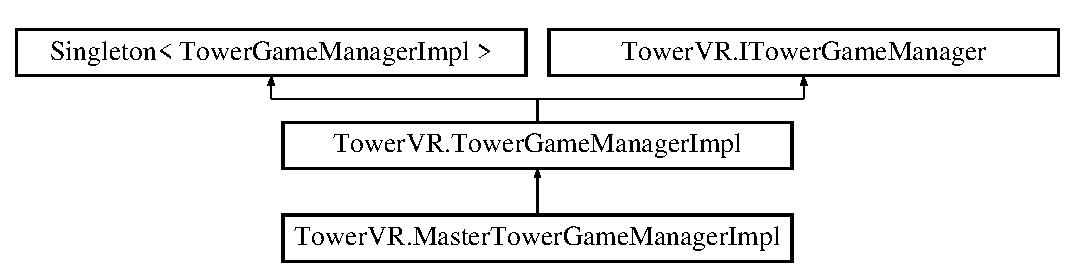
\includegraphics[height=3.000000cm]{class_tower_v_r_1_1_tower_game_manager_impl}
\end{center}
\end{figure}
\subsection*{Public Member Functions}
\begin{DoxyCompactItemize}
\item 
virtual void \hyperlink{class_tower_v_r_1_1_tower_game_manager_impl_ad4a2f3ff8f70fc26602d0c872d5cc36c}{notify\+Is\+Ready} ()
\item 
virtual void \hyperlink{class_tower_v_r_1_1_tower_game_manager_impl_a04ad123026136abf9c009ff4c03937dc}{try\+Start\+Game} ()
\item 
virtual void \hyperlink{class_tower_v_r_1_1_tower_game_manager_impl_a47563c59b6d436c05a1f70c16aeb30e9}{place\+Tower\+Piece} (float positionX, float positionZ, float rotation\+DegreesY)
\end{DoxyCompactItemize}
\subsection*{Public Attributes}
\begin{DoxyCompactItemize}
\item 
\hyperlink{class_tower_v_r_1_1_tower_game_manager}{Tower\+Game\+Manager} {\bfseries parent}\hypertarget{class_tower_v_r_1_1_tower_game_manager_impl_a97ba625071b296f357f329db279531a0}{}\label{class_tower_v_r_1_1_tower_game_manager_impl_a97ba625071b296f357f329db279531a0}

\end{DoxyCompactItemize}
\subsection*{Protected Member Functions}
\begin{DoxyCompactItemize}
\item 
virtual void {\bfseries Awake} ()\hypertarget{class_tower_v_r_1_1_tower_game_manager_impl_a3351d08f215064960524516af7e39055}{}\label{class_tower_v_r_1_1_tower_game_manager_impl_a3351d08f215064960524516af7e39055}

\item 
virtual void {\bfseries On\+Destroy} ()\hypertarget{class_tower_v_r_1_1_tower_game_manager_impl_a2aa9d1661b8b54be7309f6628a7e6128}{}\label{class_tower_v_r_1_1_tower_game_manager_impl_a2aa9d1661b8b54be7309f6628a7e6128}

\item 
virtual void \hyperlink{class_tower_v_r_1_1_tower_game_manager_impl_a325b500869bda665a71fef31783976be}{on\+Event} (byte event\+Code, object content, int sender\+ID)
\item 
virtual void {\bfseries handle\+Game\+State\+Changed\+Event} (int game\+State)\hypertarget{class_tower_v_r_1_1_tower_game_manager_impl_a1e230366e77ebf760fa5a5aacb696585}{}\label{class_tower_v_r_1_1_tower_game_manager_impl_a1e230366e77ebf760fa5a5aacb696585}

\item 
virtual void {\bfseries handle\+Turn\+State\+Changed\+Event} (int turn\+State)\hypertarget{class_tower_v_r_1_1_tower_game_manager_impl_a387b22b637c5e66e60c00ec0b3b9afa7}{}\label{class_tower_v_r_1_1_tower_game_manager_impl_a387b22b637c5e66e60c00ec0b3b9afa7}

\item 
virtual void {\bfseries handle\+Next\+Player\+Event} (int next\+Player\+ID)\hypertarget{class_tower_v_r_1_1_tower_game_manager_impl_a94c2a0d3022dd3e23095280cc5c10de4}{}\label{class_tower_v_r_1_1_tower_game_manager_impl_a94c2a0d3022dd3e23095280cc5c10de4}

\item 
virtual void {\bfseries handle\+Score\+Changed\+Event} (int player\+ID, \hyperlink{struct_tower_v_r_1_1_score}{Score} score)\hypertarget{class_tower_v_r_1_1_tower_game_manager_impl_aaec8084da6c9e63d066a327a4ceef920}{}\label{class_tower_v_r_1_1_tower_game_manager_impl_aaec8084da6c9e63d066a327a4ceef920}

\item 
virtual void {\bfseries handle\+Player\+Lost\+Event} (int player\+ID)\hypertarget{class_tower_v_r_1_1_tower_game_manager_impl_a2229c85a77dd3e8487d9d127d6a084c4}{}\label{class_tower_v_r_1_1_tower_game_manager_impl_a2229c85a77dd3e8487d9d127d6a084c4}

\item 
virtual void {\bfseries handle\+Player\+Won\+Event} (int player\+ID)\hypertarget{class_tower_v_r_1_1_tower_game_manager_impl_a048a25454703f18820253e52be426305}{}\label{class_tower_v_r_1_1_tower_game_manager_impl_a048a25454703f18820253e52be426305}

\end{DoxyCompactItemize}
\subsection*{Static Protected Member Functions}
\begin{DoxyCompactItemize}
\item 
static void {\bfseries Log\+Malformed\+Event\+Content} (string event\+Name, int sender\+ID)\hypertarget{class_tower_v_r_1_1_tower_game_manager_impl_a30fb7cdde57c78be6c01ce6cd35412ae}{}\label{class_tower_v_r_1_1_tower_game_manager_impl_a30fb7cdde57c78be6c01ce6cd35412ae}

\end{DoxyCompactItemize}
\subsection*{Additional Inherited Members}


\subsection{Detailed Description}
An \hyperlink{interface_tower_v_r_1_1_i_tower_game_manager}{I\+Tower\+Game\+Manager} that represents a remote instance.

Do not use this class directly in the game logic. 

\subsection{Member Function Documentation}
\index{Tower\+V\+R\+::\+Tower\+Game\+Manager\+Impl@{Tower\+V\+R\+::\+Tower\+Game\+Manager\+Impl}!notify\+Is\+Ready@{notify\+Is\+Ready}}
\index{notify\+Is\+Ready@{notify\+Is\+Ready}!Tower\+V\+R\+::\+Tower\+Game\+Manager\+Impl@{Tower\+V\+R\+::\+Tower\+Game\+Manager\+Impl}}
\subsubsection[{\texorpdfstring{notify\+Is\+Ready()}{notifyIsReady()}}]{\setlength{\rightskip}{0pt plus 5cm}virtual void Tower\+V\+R.\+Tower\+Game\+Manager\+Impl.\+notify\+Is\+Ready (
\begin{DoxyParamCaption}
{}
\end{DoxyParamCaption}
)\hspace{0.3cm}{\ttfamily [virtual]}}\hypertarget{class_tower_v_r_1_1_tower_game_manager_impl_ad4a2f3ff8f70fc26602d0c872d5cc36c}{}\label{class_tower_v_r_1_1_tower_game_manager_impl_ad4a2f3ff8f70fc26602d0c872d5cc36c}
Sends an event to the master client implementation. 

Implements \hyperlink{interface_tower_v_r_1_1_i_tower_game_manager_a3091c61e8ef71c592a8baf1e611489c0}{Tower\+V\+R.\+I\+Tower\+Game\+Manager}.



Reimplemented in \hyperlink{class_tower_v_r_1_1_master_tower_game_manager_impl_a318dcef324a58787554cebe80c50ef64}{Tower\+V\+R.\+Master\+Tower\+Game\+Manager\+Impl}.

\index{Tower\+V\+R\+::\+Tower\+Game\+Manager\+Impl@{Tower\+V\+R\+::\+Tower\+Game\+Manager\+Impl}!on\+Event@{on\+Event}}
\index{on\+Event@{on\+Event}!Tower\+V\+R\+::\+Tower\+Game\+Manager\+Impl@{Tower\+V\+R\+::\+Tower\+Game\+Manager\+Impl}}
\subsubsection[{\texorpdfstring{on\+Event(byte event\+Code, object content, int sender\+I\+D)}{onEvent(byte eventCode, object content, int senderID)}}]{\setlength{\rightskip}{0pt plus 5cm}virtual void Tower\+V\+R.\+Tower\+Game\+Manager\+Impl.\+on\+Event (
\begin{DoxyParamCaption}
\item[{byte}]{event\+Code, }
\item[{object}]{content, }
\item[{int}]{sender\+ID}
\end{DoxyParamCaption}
)\hspace{0.3cm}{\ttfamily [protected]}, {\ttfamily [virtual]}}\hypertarget{class_tower_v_r_1_1_tower_game_manager_impl_a325b500869bda665a71fef31783976be}{}\label{class_tower_v_r_1_1_tower_game_manager_impl_a325b500869bda665a71fef31783976be}
Receives events from the master client and alerts the observer delegates (i.\+e. Tower\+Game\+Behaviours). 

Reimplemented in \hyperlink{class_tower_v_r_1_1_master_tower_game_manager_impl_a6b6e868d063e5c3a43908c0f81349cfb}{Tower\+V\+R.\+Master\+Tower\+Game\+Manager\+Impl}.

\index{Tower\+V\+R\+::\+Tower\+Game\+Manager\+Impl@{Tower\+V\+R\+::\+Tower\+Game\+Manager\+Impl}!place\+Tower\+Piece@{place\+Tower\+Piece}}
\index{place\+Tower\+Piece@{place\+Tower\+Piece}!Tower\+V\+R\+::\+Tower\+Game\+Manager\+Impl@{Tower\+V\+R\+::\+Tower\+Game\+Manager\+Impl}}
\subsubsection[{\texorpdfstring{place\+Tower\+Piece(float position\+X, float position\+Z, float rotation\+Degrees\+Y)}{placeTowerPiece(float positionX, float positionZ, float rotationDegreesY)}}]{\setlength{\rightskip}{0pt plus 5cm}virtual void Tower\+V\+R.\+Tower\+Game\+Manager\+Impl.\+place\+Tower\+Piece (
\begin{DoxyParamCaption}
\item[{float}]{positionX, }
\item[{float}]{positionZ, }
\item[{float}]{rotation\+DegreesY}
\end{DoxyParamCaption}
)\hspace{0.3cm}{\ttfamily [virtual]}}\hypertarget{class_tower_v_r_1_1_tower_game_manager_impl_a47563c59b6d436c05a1f70c16aeb30e9}{}\label{class_tower_v_r_1_1_tower_game_manager_impl_a47563c59b6d436c05a1f70c16aeb30e9}
Sends an event to the master client implementation. 

Implements \hyperlink{interface_tower_v_r_1_1_i_tower_game_manager_aa800aded89d5de4af84321110f6eadd0}{Tower\+V\+R.\+I\+Tower\+Game\+Manager}.



Reimplemented in \hyperlink{class_tower_v_r_1_1_master_tower_game_manager_impl_a653a15c9e2af6c11bbd9678cd54a716b}{Tower\+V\+R.\+Master\+Tower\+Game\+Manager\+Impl}.

\index{Tower\+V\+R\+::\+Tower\+Game\+Manager\+Impl@{Tower\+V\+R\+::\+Tower\+Game\+Manager\+Impl}!try\+Start\+Game@{try\+Start\+Game}}
\index{try\+Start\+Game@{try\+Start\+Game}!Tower\+V\+R\+::\+Tower\+Game\+Manager\+Impl@{Tower\+V\+R\+::\+Tower\+Game\+Manager\+Impl}}
\subsubsection[{\texorpdfstring{try\+Start\+Game()}{tryStartGame()}}]{\setlength{\rightskip}{0pt plus 5cm}virtual void Tower\+V\+R.\+Tower\+Game\+Manager\+Impl.\+try\+Start\+Game (
\begin{DoxyParamCaption}
{}
\end{DoxyParamCaption}
)\hspace{0.3cm}{\ttfamily [virtual]}}\hypertarget{class_tower_v_r_1_1_tower_game_manager_impl_a04ad123026136abf9c009ff4c03937dc}{}\label{class_tower_v_r_1_1_tower_game_manager_impl_a04ad123026136abf9c009ff4c03937dc}
Sends an event to the master client implementation. 

Implements \hyperlink{interface_tower_v_r_1_1_i_tower_game_manager_a3b5866dd2b9659d65982f4ff651ee2c9}{Tower\+V\+R.\+I\+Tower\+Game\+Manager}.



Reimplemented in \hyperlink{class_tower_v_r_1_1_master_tower_game_manager_impl_a43cb29dc14b7d9dcd90b5826c49a380d}{Tower\+V\+R.\+Master\+Tower\+Game\+Manager\+Impl}.



The documentation for this class was generated from the following file\+:\begin{DoxyCompactItemize}
\item 
/\+Users/benjamin/\+Programmering/\+Android\+H\+M\+D/\+Tower\+V\+R/\+Assets/\+Scripts/\+Custom/\+Game/\+Tower/\+Manager/\+Impl/Tower\+Game\+Manager\+Impl.\+cs\end{DoxyCompactItemize}

\hypertarget{class_tower_v_r_1_1_tower_piece}{}\section{Tower\+V\+R.\+Tower\+Piece Class Reference}
\label{class_tower_v_r_1_1_tower_piece}\index{Tower\+V\+R.\+Tower\+Piece@{Tower\+V\+R.\+Tower\+Piece}}
Inheritance diagram for Tower\+V\+R.\+Tower\+Piece\+:\begin{figure}[H]
\begin{center}
\leavevmode
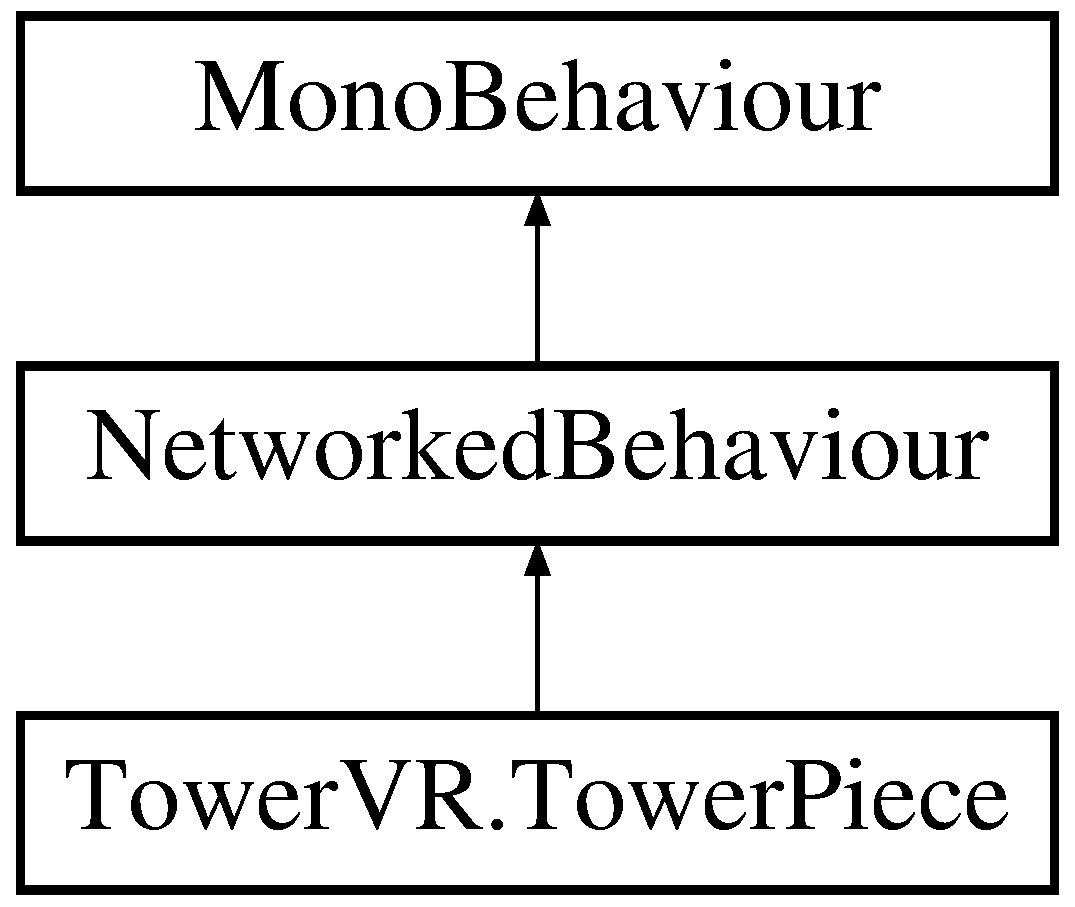
\includegraphics[height=3.000000cm]{class_tower_v_r_1_1_tower_piece}
\end{center}
\end{figure}
\subsection*{Static Public Member Functions}
\begin{DoxyCompactItemize}
\item 
static \hyperlink{class_tower_v_r_1_1_tower_piece}{Tower\+Piece} \hyperlink{class_tower_v_r_1_1_tower_piece_a686d6c1c40c7a45e6b3bb9f31b79b12d}{Create} (\hyperlink{class_tower_v_r_1_1_tower_piece_info}{Tower\+Piece\+Info} info, Material material)
\end{DoxyCompactItemize}
\subsection*{Properties}
\begin{DoxyCompactItemize}
\item 
Tower\+Piece\+Difficulty {\bfseries difficulty}\hspace{0.3cm}{\ttfamily  \mbox{[}get\mbox{]}}\hypertarget{class_tower_v_r_1_1_tower_piece_a80a1261ef724785a25d02a36cf26f7a1}{}\label{class_tower_v_r_1_1_tower_piece_a80a1261ef724785a25d02a36cf26f7a1}

\item 
Mesh\+Filter {\bfseries mesh\+Filter}\hspace{0.3cm}{\ttfamily  \mbox{[}get\mbox{]}}\hypertarget{class_tower_v_r_1_1_tower_piece_a6cd90f25eb69ac26afcc1c13c4fe7054}{}\label{class_tower_v_r_1_1_tower_piece_a6cd90f25eb69ac26afcc1c13c4fe7054}

\item 
Mesh\+Collider {\bfseries mesh\+Collider}\hspace{0.3cm}{\ttfamily  \mbox{[}get\mbox{]}}\hypertarget{class_tower_v_r_1_1_tower_piece_a2165bbc9011d19cc2afc87b6400200a1}{}\label{class_tower_v_r_1_1_tower_piece_a2165bbc9011d19cc2afc87b6400200a1}

\item 
Material {\bfseries material}\hspace{0.3cm}{\ttfamily  \mbox{[}get\mbox{]}}\hypertarget{class_tower_v_r_1_1_tower_piece_a87cc9ad884bd6a1bcff5fd6ed809314b}{}\label{class_tower_v_r_1_1_tower_piece_a87cc9ad884bd6a1bcff5fd6ed809314b}

\end{DoxyCompactItemize}


\subsection{Detailed Description}
Marker class for a Tower Piece.

This component should be attached to a Game\+Object that has a mesh, a mesh collider and a material. 

\subsection{Member Function Documentation}
\index{Tower\+V\+R\+::\+Tower\+Piece@{Tower\+V\+R\+::\+Tower\+Piece}!Create@{Create}}
\index{Create@{Create}!Tower\+V\+R\+::\+Tower\+Piece@{Tower\+V\+R\+::\+Tower\+Piece}}
\subsubsection[{\texorpdfstring{Create(\+Tower\+Piece\+Info info, Material material)}{Create(TowerPieceInfo info, Material material)}}]{\setlength{\rightskip}{0pt plus 5cm}static {\bf Tower\+Piece} Tower\+V\+R.\+Tower\+Piece.\+Create (
\begin{DoxyParamCaption}
\item[{{\bf Tower\+Piece\+Info}}]{info, }
\item[{Material}]{material}
\end{DoxyParamCaption}
)\hspace{0.3cm}{\ttfamily [static]}}\hypertarget{class_tower_v_r_1_1_tower_piece_a686d6c1c40c7a45e6b3bb9f31b79b12d}{}\label{class_tower_v_r_1_1_tower_piece_a686d6c1c40c7a45e6b3bb9f31b79b12d}
Instantiates a new Game\+Object and configures it as a tower piece with the specified info. 

The documentation for this class was generated from the following file\+:\begin{DoxyCompactItemize}
\item 
/\+Users/benjamin/\+Programmering/\+Android\+H\+M\+D/\+Tower\+V\+R/\+Assets/\+Scripts/\+Custom/\+Game/\+Tower/Tower\+Piece.\+cs\end{DoxyCompactItemize}

\hypertarget{class_tower_v_r_1_1_tower_piece_info}{}\section{Tower\+V\+R.\+Tower\+Piece\+Info Class Reference}
\label{class_tower_v_r_1_1_tower_piece_info}\index{Tower\+V\+R.\+Tower\+Piece\+Info@{Tower\+V\+R.\+Tower\+Piece\+Info}}
Inheritance diagram for Tower\+V\+R.\+Tower\+Piece\+Info\+:\begin{figure}[H]
\begin{center}
\leavevmode
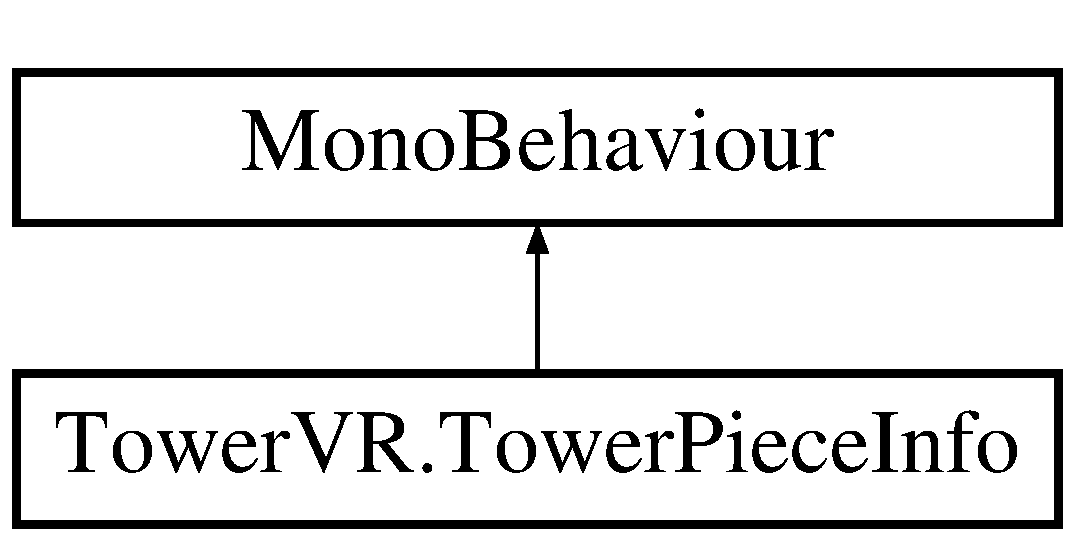
\includegraphics[height=2.000000cm]{class_tower_v_r_1_1_tower_piece_info}
\end{center}
\end{figure}
\subsection*{Public Attributes}
\begin{DoxyCompactItemize}
\item 
Mesh {\bfseries mesh}\hypertarget{class_tower_v_r_1_1_tower_piece_info_a9a51d7505e2ab6497753a04fc5d0bda8}{}\label{class_tower_v_r_1_1_tower_piece_info_a9a51d7505e2ab6497753a04fc5d0bda8}

\item 
Tower\+Piece\+Difficulty {\bfseries difficulty}\hypertarget{class_tower_v_r_1_1_tower_piece_info_a0c14a859f276fa25a4c179b1760285bd}{}\label{class_tower_v_r_1_1_tower_piece_info_a0c14a859f276fa25a4c179b1760285bd}

\end{DoxyCompactItemize}


\subsection{Detailed Description}
Class representing a playable/placable tower piece.

It contains a reference to a mesh as well as a difficulty. 

The documentation for this class was generated from the following file\+:\begin{DoxyCompactItemize}
\item 
/\+Users/benjamin/\+Programmering/\+Android\+H\+M\+D/\+Tower\+V\+R/\+Assets/\+Scripts/\+Custom/\+Game/\+Tower/Tower\+Piece\+Info.\+cs\end{DoxyCompactItemize}

\hypertarget{class_tower_v_r_1_1_tower_piece_spawner}{}\section{Tower\+V\+R.\+Tower\+Piece\+Spawner Class Reference}
\label{class_tower_v_r_1_1_tower_piece_spawner}\index{Tower\+V\+R.\+Tower\+Piece\+Spawner@{Tower\+V\+R.\+Tower\+Piece\+Spawner}}
Inheritance diagram for Tower\+V\+R.\+Tower\+Piece\+Spawner\+:\begin{figure}[H]
\begin{center}
\leavevmode
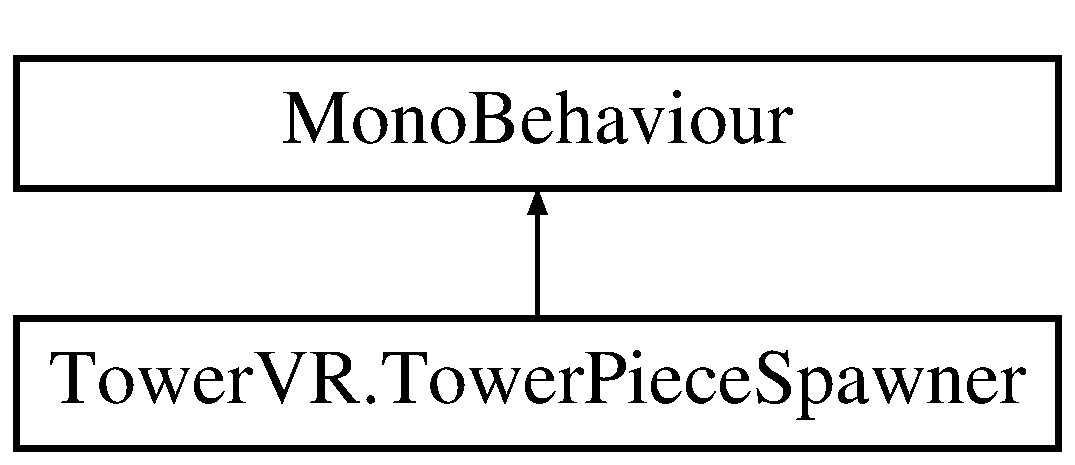
\includegraphics[height=2.000000cm]{class_tower_v_r_1_1_tower_piece_spawner}
\end{center}
\end{figure}
\subsection*{Public Member Functions}
\begin{DoxyCompactItemize}
\item 
void {\bfseries Network\+\_\+\+Spawn\+Tower\+Piece} (Vector3 position, Vector3 euler\+Angles, Tower\+Piece\+Difficulty difficulty)\hypertarget{class_tower_v_r_1_1_tower_piece_spawner_a262d0e9b14f814ec49bc572d906d74f3}{}\label{class_tower_v_r_1_1_tower_piece_spawner_a262d0e9b14f814ec49bc572d906d74f3}

\item 
void {\bfseries Network\+\_\+\+Spawn\+Tower\+Piece} (Vector3 position, Vector3 euler\+Angles)\hypertarget{class_tower_v_r_1_1_tower_piece_spawner_aa167d6fdd1cd667dab34e935d9f82f57}{}\label{class_tower_v_r_1_1_tower_piece_spawner_aa167d6fdd1cd667dab34e935d9f82f57}

\item 
void {\bfseries On\+Connected\+To\+Master} ()\hypertarget{class_tower_v_r_1_1_tower_piece_spawner_a5318d7725ba9f0b6d0f215536c16a7a6}{}\label{class_tower_v_r_1_1_tower_piece_spawner_a5318d7725ba9f0b6d0f215536c16a7a6}

\item 
void {\bfseries On\+Joined\+Room} ()\hypertarget{class_tower_v_r_1_1_tower_piece_spawner_a91f9b22165e13b30aebe5f52c5ab1805}{}\label{class_tower_v_r_1_1_tower_piece_spawner_a91f9b22165e13b30aebe5f52c5ab1805}

\end{DoxyCompactItemize}
\subsection*{Public Attributes}
\begin{DoxyCompactItemize}
\item 
List$<$ Material $>$ {\bfseries materials}\hypertarget{class_tower_v_r_1_1_tower_piece_spawner_a61ce0fc19fb1800a95cb74efc7a7ab6f}{}\label{class_tower_v_r_1_1_tower_piece_spawner_a61ce0fc19fb1800a95cb74efc7a7ab6f}

\item 
List$<$ \hyperlink{class_tower_v_r_1_1_tower_piece_info}{Tower\+Piece\+Info} $>$ {\bfseries tower\+Piece\+Infos}\hypertarget{class_tower_v_r_1_1_tower_piece_spawner_a2ce360a9da394be0169dac4f2bf4ca2d}{}\label{class_tower_v_r_1_1_tower_piece_spawner_a2ce360a9da394be0169dac4f2bf4ca2d}

\end{DoxyCompactItemize}


The documentation for this class was generated from the following file\+:\begin{DoxyCompactItemize}
\item 
/\+Users/benjamin/\+Programmering/\+Android\+H\+M\+D/\+Tower\+V\+R/\+Assets/\+Scripts/\+Custom/\+Game/\+Tower/Tower\+Piece\+Spawner.\+cs\end{DoxyCompactItemize}

\hypertarget{class_transform_debugger}{}\section{Transform\+Debugger Class Reference}
\label{class_transform_debugger}\index{Transform\+Debugger@{Transform\+Debugger}}
Inheritance diagram for Transform\+Debugger\+:\begin{figure}[H]
\begin{center}
\leavevmode
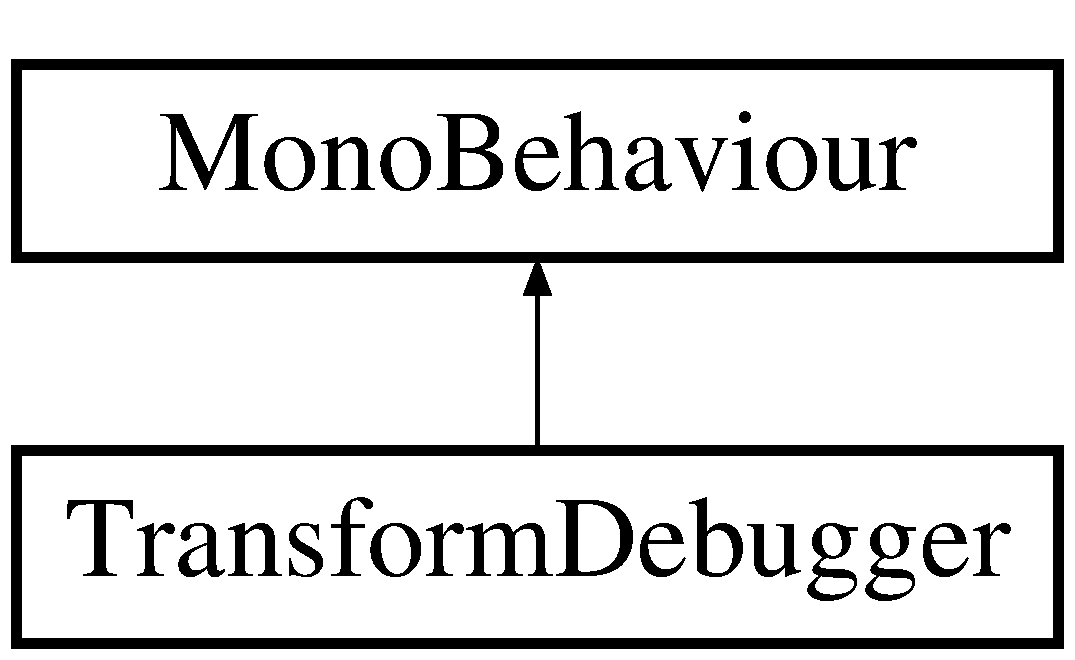
\includegraphics[height=2.000000cm]{class_transform_debugger}
\end{center}
\end{figure}
\subsection*{Public Attributes}
\begin{DoxyCompactItemize}
\item 
bool {\bfseries use\+Custom\+Debug\+Interval} = false\hypertarget{class_transform_debugger_aaf06d9c33dc9447d44bb7449ecf2c141}{}\label{class_transform_debugger_aaf06d9c33dc9447d44bb7449ecf2c141}

\item 
float {\bfseries update\+Interval\+Seconds} = 1.\+0f\hypertarget{class_transform_debugger_a73ef663cb15c97e23c7c64062909a3a2}{}\label{class_transform_debugger_a73ef663cb15c97e23c7c64062909a3a2}

\item 
bool {\bfseries debug\+Position}\hypertarget{class_transform_debugger_ad1f6c8c9bcb39453ce66aaa3d3568421}{}\label{class_transform_debugger_ad1f6c8c9bcb39453ce66aaa3d3568421}

\item 
bool {\bfseries debug\+Rotation}\hypertarget{class_transform_debugger_ad32a74a860e5d8dbfcf5e25e968115f9}{}\label{class_transform_debugger_ad32a74a860e5d8dbfcf5e25e968115f9}

\item 
bool {\bfseries debug\+Scale}\hypertarget{class_transform_debugger_a1a2e3f97f561dcb247d6eddaae0fc585}{}\label{class_transform_debugger_a1a2e3f97f561dcb247d6eddaae0fc585}

\end{DoxyCompactItemize}


The documentation for this class was generated from the following file\+:\begin{DoxyCompactItemize}
\item 
/\+Users/benjamin/\+Programmering/\+Android\+H\+M\+D/\+Tower\+V\+R/\+Assets/\+Scripts/\+Custom/\+Generic/Transform\+Debugger.\+cs\end{DoxyCompactItemize}

\hypertarget{class_tower_v_r_1_1_try_start_game_event}{}\section{Tower\+V\+R.\+Try\+Start\+Game\+Event Class Reference}
\label{class_tower_v_r_1_1_try_start_game_event}\index{Tower\+V\+R.\+Try\+Start\+Game\+Event@{Tower\+V\+R.\+Try\+Start\+Game\+Event}}
Inheritance diagram for Tower\+V\+R.\+Try\+Start\+Game\+Event\+:\begin{figure}[H]
\begin{center}
\leavevmode
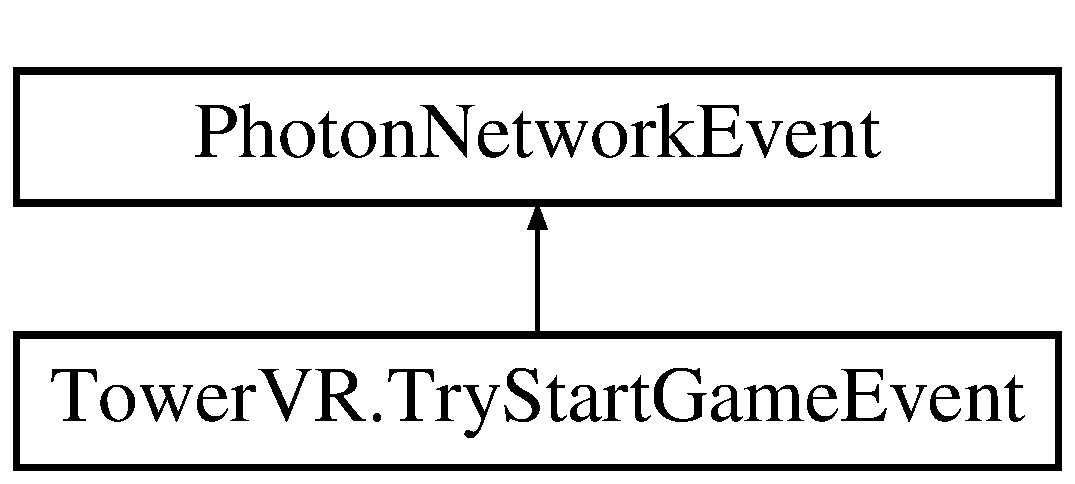
\includegraphics[height=2.000000cm]{class_tower_v_r_1_1_try_start_game_event}
\end{center}
\end{figure}
\subsection*{Additional Inherited Members}


\subsection{Detailed Description}
Event that alerts the master client and tries to start the game. 

The documentation for this class was generated from the following file\+:\begin{DoxyCompactItemize}
\item 
/\+Users/benjamin/\+Programmering/\+Android\+H\+M\+D/\+Tower\+V\+R/\+Assets/\+Scripts/\+Custom/\+Game/\+Network/\+Events/Try\+Start\+Game\+Event.\+cs\end{DoxyCompactItemize}

\hypertarget{class_tower_v_r_1_1_turn_state}{}\section{Tower\+V\+R.\+Turn\+State Class Reference}
\label{class_tower_v_r_1_1_turn_state}\index{Tower\+V\+R.\+Turn\+State@{Tower\+V\+R.\+Turn\+State}}
\subsection*{Static Public Member Functions}
\begin{DoxyCompactItemize}
\item 
static bool {\bfseries Is\+Valid} (int potential\+Turn\+State)\hypertarget{class_tower_v_r_1_1_turn_state_a203c3369f5ef29df16e72a4ee8427f58}{}\label{class_tower_v_r_1_1_turn_state_a203c3369f5ef29df16e72a4ee8427f58}

\item 
static string {\bfseries To\+String} (int turn\+State)\hypertarget{class_tower_v_r_1_1_turn_state_a0d8995c30ef7e1af0d2dda5c4bb8150e}{}\label{class_tower_v_r_1_1_turn_state_a0d8995c30ef7e1af0d2dda5c4bb8150e}

\end{DoxyCompactItemize}
\subsection*{Public Attributes}
\begin{DoxyCompactItemize}
\item 
const int {\bfseries Not\+Started} = 0\hypertarget{class_tower_v_r_1_1_turn_state_a8df0d8eddb9324e7a9006ac62751a73c}{}\label{class_tower_v_r_1_1_turn_state_a8df0d8eddb9324e7a9006ac62751a73c}

\item 
const int {\bfseries Selecting\+Tower\+Piece} = 1\hypertarget{class_tower_v_r_1_1_turn_state_a131a4d02f0c537275e453d1c6aa5c535}{}\label{class_tower_v_r_1_1_turn_state_a131a4d02f0c537275e453d1c6aa5c535}

\item 
const int {\bfseries Placing\+Tower\+Piece} = 2\hypertarget{class_tower_v_r_1_1_turn_state_a7594dc7af385691556c9ab21d477e93f}{}\label{class_tower_v_r_1_1_turn_state_a7594dc7af385691556c9ab21d477e93f}

\item 
const int {\bfseries Tower\+Reacting} = 3\hypertarget{class_tower_v_r_1_1_turn_state_a9ac24dc02210ce472b97236e16381d4f}{}\label{class_tower_v_r_1_1_turn_state_a9ac24dc02210ce472b97236e16381d4f}

\end{DoxyCompactItemize}


The documentation for this class was generated from the following file\+:\begin{DoxyCompactItemize}
\item 
/\+Users/benjamin/\+Programmering/\+Android\+H\+M\+D/\+Tower\+V\+R/\+Assets/\+Scripts/\+Custom/\+Game/States.\+cs\end{DoxyCompactItemize}

\hypertarget{class_tower_v_r_1_1_turn_state_changed_event}{}\section{Tower\+V\+R.\+Turn\+State\+Changed\+Event Class Reference}
\label{class_tower_v_r_1_1_turn_state_changed_event}\index{Tower\+V\+R.\+Turn\+State\+Changed\+Event@{Tower\+V\+R.\+Turn\+State\+Changed\+Event}}
Inheritance diagram for Tower\+V\+R.\+Turn\+State\+Changed\+Event\+:\begin{figure}[H]
\begin{center}
\leavevmode
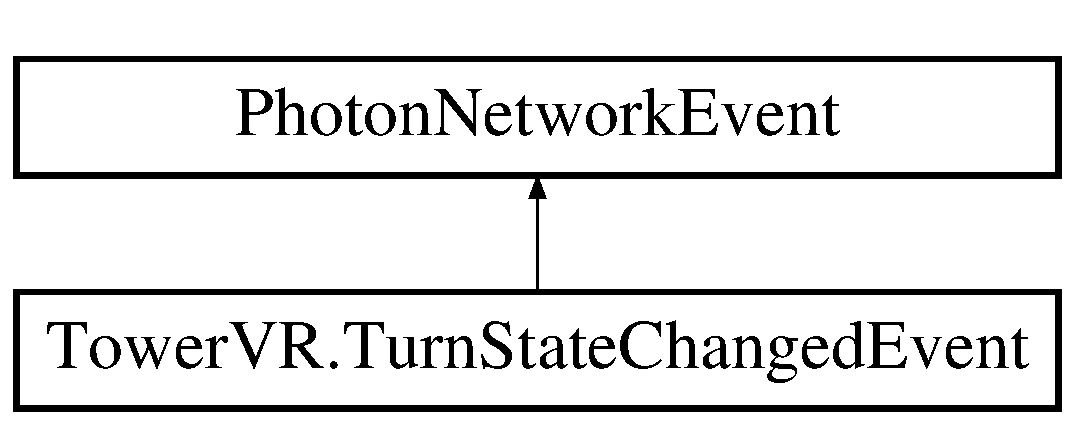
\includegraphics[height=2.000000cm]{class_tower_v_r_1_1_turn_state_changed_event}
\end{center}
\end{figure}
\subsection*{Public Member Functions}
\begin{DoxyCompactItemize}
\item 
{\bfseries Turn\+State\+Changed\+Event} (int valid\+Turn\+State)\hypertarget{class_tower_v_r_1_1_turn_state_changed_event_a52ab33a4e06c8e369f475917625e1ad1}{}\label{class_tower_v_r_1_1_turn_state_changed_event_a52ab33a4e06c8e369f475917625e1ad1}

\end{DoxyCompactItemize}
\subsection*{Static Public Member Functions}
\begin{DoxyCompactItemize}
\item 
static bool \hyperlink{class_tower_v_r_1_1_turn_state_changed_event_af2a87f4c766ea138684caf2a79efeed7}{Try\+Parse} (object obj, out int new\+Turn\+State)
\end{DoxyCompactItemize}
\subsection*{Additional Inherited Members}


\subsection{Detailed Description}
An event raised when the master client has changed the current turn\textquotesingle{}s state. 

\subsection{Member Function Documentation}
\index{Tower\+V\+R\+::\+Turn\+State\+Changed\+Event@{Tower\+V\+R\+::\+Turn\+State\+Changed\+Event}!Try\+Parse@{Try\+Parse}}
\index{Try\+Parse@{Try\+Parse}!Tower\+V\+R\+::\+Turn\+State\+Changed\+Event@{Tower\+V\+R\+::\+Turn\+State\+Changed\+Event}}
\subsubsection[{\texorpdfstring{Try\+Parse(object obj, out int new\+Turn\+State)}{TryParse(object obj, out int newTurnState)}}]{\setlength{\rightskip}{0pt plus 5cm}static bool Tower\+V\+R.\+Turn\+State\+Changed\+Event.\+Try\+Parse (
\begin{DoxyParamCaption}
\item[{object}]{obj, }
\item[{out int}]{new\+Turn\+State}
\end{DoxyParamCaption}
)\hspace{0.3cm}{\ttfamily [static]}}\hypertarget{class_tower_v_r_1_1_turn_state_changed_event_af2a87f4c766ea138684caf2a79efeed7}{}\label{class_tower_v_r_1_1_turn_state_changed_event_af2a87f4c766ea138684caf2a79efeed7}
Tries to parse the contents of the event. 

The documentation for this class was generated from the following file\+:\begin{DoxyCompactItemize}
\item 
/\+Users/benjamin/\+Programmering/\+Android\+H\+M\+D/\+Tower\+V\+R/\+Assets/\+Scripts/\+Custom/\+Game/\+Network/\+Events/Turn\+State\+Changed\+Event.\+cs\end{DoxyCompactItemize}

\hypertarget{class_tower_v_r_1_1_turn_time_limits}{}\section{Tower\+V\+R.\+Turn\+Time\+Limits Class Reference}
\label{class_tower_v_r_1_1_turn_time_limits}\index{Tower\+V\+R.\+Turn\+Time\+Limits@{Tower\+V\+R.\+Turn\+Time\+Limits}}
\subsection*{Public Attributes}
\begin{DoxyCompactItemize}
\item 
const float {\bfseries Selecting\+Tower\+Piece} = 2.\+0f\hypertarget{class_tower_v_r_1_1_turn_time_limits_ae3c0742a7d389534a0b3b1c4d229dc32}{}\label{class_tower_v_r_1_1_turn_time_limits_ae3c0742a7d389534a0b3b1c4d229dc32}

\item 
const float {\bfseries Placing\+Tower\+Piece} = 3.\+0f\hypertarget{class_tower_v_r_1_1_turn_time_limits_a90c299e1f4b47955972087aaee4c81e4}{}\label{class_tower_v_r_1_1_turn_time_limits_a90c299e1f4b47955972087aaee4c81e4}

\item 
const float {\bfseries Tower\+Reacting} = 5.\+0f\hypertarget{class_tower_v_r_1_1_turn_time_limits_a18f1e3032ab93929fd42da3da442461a}{}\label{class_tower_v_r_1_1_turn_time_limits_a18f1e3032ab93929fd42da3da442461a}

\end{DoxyCompactItemize}


The documentation for this class was generated from the following file\+:\begin{DoxyCompactItemize}
\item 
/\+Users/benjamin/\+Programmering/\+Android\+H\+M\+D/\+Tower\+V\+R/\+Assets/\+Scripts/\+Custom/\+Game/Tower\+Game\+Constants.\+cs\end{DoxyCompactItemize}

%--- End generated contents ---

% Index
\backmatter
\newpage
\phantomsection
\clearemptydoublepage
\addcontentsline{toc}{chapter}{Index}
\printindex

\end{document}
